\documentclass[notes]{ituphd}
\usepackage{dtcnotes}
\usepgfplotslibrary{groupplots}

% ---------------------------------------------------------------------------
% Course information (edit your name here)
% ---------------------------------------------------------------------------
\coursetitle{Discrete-Time Control Systems}
\coursecode{KOM3781}
\semester{2019--20 Fall}
\ituunit{Y{\i}ld{\i}z Technical University, Control and Automation Engineering}
\renewcommand{\itulogofile}{}      % these notes are from a YTU course: no ITU logo
%\renewcommand{\itulogofile}{itu-blue.pdf}   % <- uncomment to put the ITU logo back

\title{Lecture Notes}
\author{Mert Serhat Sarıhan}
\instructor{Dr. M. Tolga Emirler}
\date{Typeset \today}

\begin{document}
\makecover
\tableofcontents
\clearpage

\section*{About these notes}
\addcontentsline{toc}{section}{About these notes}
These are the typeset version of my handwritten notes of the course
\emph{KOM3781 Discrete-Time Control Systems}. The content and the order follow the handwritten
notes (87 pages, September--December 2019), which in turn follow Ogata,
\emph{Discrete-Time Control Systems}, and Fadali, \emph{Digital Control Engineering}.
Nothing from the board was dropped.


\section{Data Acquisition, Conversion and Distribution}\label{sec:acq}
\lecdate{23 September 2019}

\subsection{Quantizing and quantization error}\scanref{pp.\,1}
The main function of an A/D conversion consists of three steps.
\begin{itemize}
  \item \textbf{Sampling:} the analog signal becomes a discrete-time signal (real numbers).
  \item \textbf{Amplitude quantization:} each number is replaced by an approximation taken from a finite
        set of discrete values. This causes the \emph{quantization error}.
  \item \textbf{Coding:} the discrete values are converted to binary values.
\end{itemize}

\paragraph{Quantization level.} With $\mathrm{FSR}$ the full-scale range and $n$ the number of bits,
\begin{equation}
  Q=\frac{\mathrm{FSR}}{2^{n}} .
\end{equation}

\begin{example}
For an input range of $\pm5\,\mathrm{V}$ (so $\mathrm{FSR}=10\,\mathrm{V}$) and a $12$-bit A/D converter (ADC),
\[
  Q=\frac{10}{2^{12}}=2.44\ \mathrm{mV}.
\]
This ADC cannot generate a new discrete value if the voltage change between two adjacent sample values is
smaller than $2.44\ \mathrm{mV}$.
\end{example}

\paragraph{Quantization error.} Let $x(t)$ be the analog input and $y(t)$ the closest available digital
value at the output of the A/D block. The error is $e(t)=x(t)-y(t)$. It varies between $0$ and $\mp\tfrac12 Q$,
so its magnitude satisfies
\begin{equation}
  0\le \lvert e(t)\rvert\le \tfrac12 Q .
\end{equation}

\begin{center}
\begin{tikzpicture}[scale=1]
  \begin{axis}[width=0.78\linewidth,height=5.6cm,axis lines=left,xlabel={$x(t)$ (analog input)},
      ylabel={$y(t)$ (digital value)},xmin=0,xmax=8,ymin=0,ymax=8.6,
      xtick={0,1,...,8},ytick={0,1,...,8},
      xticklabels={0,,,,,,,,},yticklabels={0,,,,,,,,},grid=both,
      grid style={very thin,gridgray},every axis plot/.append style={thick}]
    \addplot[itublue,const plot mark mid,domain=0:8,samples=17,unbounded coords=jump]
      {round(x)};
    \addplot[itugold,dashed,domain=0:8] {x};
    \node[font=\small,itublue,anchor=west] at (axis cs:4.7,2.5) {$y=$ quantized};
    \node[font=\small,itugold,anchor=west] at (axis cs:1.1,5.4) {$y=x$ (ideal)};
    \draw[<->,boardgreen,thick] (axis cs:5.2,5.2) -- node[right,font=\scriptsize]{$Q$} (axis cs:5.2,6.2);
  \end{axis}
\end{tikzpicture}\\[2pt]
{\small Staircase characteristic of a quantizer; the step is $Q$ and the error never exceeds $Q/2$.}
\end{center}

\begin{addsol}
\textbf{Problem.} Find $Q$ for a $\pm5\,\mathrm{V}$ converter with $n=8,10,12,16$ bits, and the number of
levels $2^n$.

\medskip
\begin{center}
\begin{tabular}{@{}rrr@{}}\toprule
$n$ & $2^n$ & $Q=10/2^n$ \\ \midrule
8  & 256    & 39.06 mV \\
10 & 1024   & 9.77 mV \\
12 & 4096   & 2.44 mV \\
16 & 65536  & 0.153 mV \\ \bottomrule
\end{tabular}
\end{center}
The maximum error is $Q/2$, e.g.\ $1.22\,\mathrm{mV}$ for $n=12$.
\end{addsol}

%------------------------------------------------------------------------------
\subsection{Data acquisition, conversion and distribution systems}\scanref{pp.\,2--6}
The signal conversion in a digital control system involves the following operations:
\begin{enumerate}
  \item Multiplexing and demultiplexing,
  \item Sample and hold,
  \item A/D conversion (quantizing, encoding),
  \item D/A conversion (decoding).
\end{enumerate}

\paragraph{Data-acquisition system.} Physical variables (position, acceleration, temperature, pressure,
\ldots) are converted to a voltage or current by a transducer, amplified, low-pass filtered (noise
cancellation), multiplexed, sampled-and-held and finally converted by the A/D converter before they go to
the digital controller.

\begin{center}
\resizebox{\linewidth}{!}{\begin{tikzpicture}[node distance=13mm,font=\small]
  \node[blk,minimum height=9mm] (tr) {Transducer};
  \node[blk,right=of tr] (am) {Amplifier};
  \node[blk,right=of am,text width=17mm] (lp) {Low Pass Filter};
  \node[blk,right=of lp] (mux) {Analog MUX};
  \node[blk,right=of mux] (sh) {Sample Hold};
  \draw[sig] ($(tr.west)+(-8mm,0)$) -- node[above,pos=0.2,text width=13mm,align=center,font=\scriptsize]{physical variables} (tr);
  \draw[sig] (tr) -- node[above,font=\scriptsize,align=center]{voltage\\ or current} (am);
  \draw[sig] (am) -- (lp);
  \draw[sig] (lp) -- node[below,font=\scriptsize]{noise cancel.} (mux);
  \draw[sig] (mux) -- (sh);
  \node[blk,below=9mm of sh] (adc) {A/D Conv.};
  \draw[sig] (sh) -- (adc);
  \draw[sig] (adc.west) -- ++(-8mm,0) node[left,font=\scriptsize,align=center]{to digital\\control};
  \draw[sig] ($(mux.north)+(0,5mm)$) node[above,font=\scriptsize]{Analog} -- (mux.north);
  \node[font=\scriptsize,right=1mm of adc] {Digital};
\end{tikzpicture}}
\end{center}

\paragraph{Data-distribution system.} The digital value from the controller is stored in a register,
demultiplexed, converted by D/A converters and held before it reaches the actuator.

\begin{center}
\resizebox{\linewidth}{!}{\begin{tikzpicture}[node distance=13mm,font=\small]
  \node[blk] (rg) {Register};
  \node[blk,right=of rg] (dm) {DeMUX};
  \node[blk,right=of dm] (da) {D/A conv.};
  \node[blk,right=of da] (hd) {Hold};
  \draw[sig] ($(rg.west)+(-10mm,0)$) -- node[above,pos=0.1,font=\scriptsize,align=center]{from digital\\control} (rg);
  \draw[sig] (rg) -- (dm);
  \draw[sig] (dm) -- node[above,font=\scriptsize]{Digital} (da);
  \draw[sig] (da) -- (hd);
  \draw[sig] (hd) -- node[above,font=\scriptsize,pos=0.5]{Analog} ++(1.8,0) node[right,font=\scriptsize,align=left]{to\\actuator};
\end{tikzpicture}}
\end{center}

%------------------------------------------------------------------------------
\subsubsection*{Analog multiplexer (MUX)}
\begin{itemize}
  \item It is a multiple switch (usually an electronic switch) that sequentially switches among many analog
        input channels.
  \item Number of channels: $4,8,16,32,64,\dots$
  \item At a given instant only one switch is in the ``on'' position.
\end{itemize}

\begin{center}
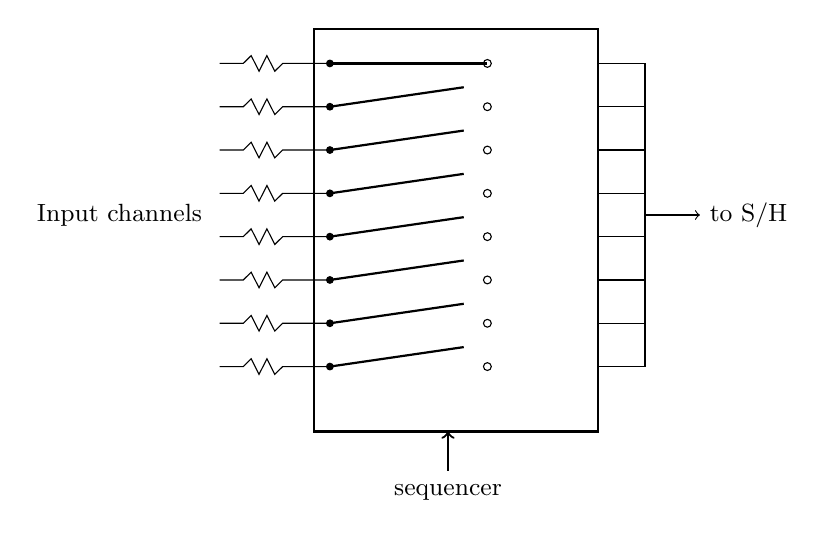
\begin{tikzpicture}[x=1cm,y=0.55cm]
  \draw[thick] (0,-0.7) rectangle (3.6,8.6);
  \foreach \i in {0,...,7} {
    \pgfmathsetmacro{\yy}{7.8-\i}
    \draw (-1.2,\yy) -- ++(0.3,0) -- ++(0.1,0.18) -- ++(0.1,-0.36) -- ++(0.1,0.36) -- ++(0.1,-0.36) -- ++(0.1,0.18) -- (0.2,\yy);
    \node[circle,fill,inner sep=1pt] at (0.2,\yy) {};
    \node[circle,draw,inner sep=1pt] at (2.2,\yy) {};
    \draw (3.6,\yy) -- (4.2,\yy);
    \ifnum\i=0
      \draw[thick] (0.2,\yy) -- (2.2,\yy);
    \else
      \draw[thick] (0.2,\yy) -- ($(0.2,\yy)+(1.7,0.45)$);
    \fi
  }
  \draw[thick] (4.2,0.8) -- (4.2,7.8);
  \draw[->] (4.2,4.3) -- (4.9,4.3) node[right,font=\small]{to S/H};
  \node[font=\small,anchor=east] at (-1.3,4.3) {Input channels};
  \draw[->,thick] (1.7,-1.6) -- (1.7,-0.7);
  \node[font=\small] at (1.7,-2.1) {sequencer};
\end{tikzpicture}
\end{center}

\subsubsection*{Demultiplexer}
It separates the composite output digital data from the digital controller into the original channels. Each
channel is connected to a D/A converter to produce the analog signal of that channel.

\begin{center}
\begin{tikzpicture}[font=\small]
  \node[blk,minimum width=10mm] (d1) at (0,0.7) {DAC};
  \node[blk,minimum width=10mm] (d2) at (0,-0.1) {DAC};
  \draw[sig] (-1.6,0.7) -- (d1); \draw[sig] (-1.6,-0.1) -- (d2);
  \draw[thick] (-1.6,0.7) -- (-1.6,-1.1);
  \draw[sig] (-2.2,-0.2) -- (-1.6,-0.2);
  \draw[sig] (-1.6,-0.9) -- (-1.1,-0.9) node[right]{\vdots};
  \draw[sig] (d1) -- ++(1.2,0) node[right]{Analog 1};
  \draw[sig] (d2) -- ++(1.2,0) node[right]{Analog 2};
\end{tikzpicture}
\end{center}

\subsubsection*{Sample-and-hold circuit}
A sampler converts an analog signal into a train of amplitude-modulated pulses. The hold circuit holds the
value of the sampled pulse over a specified period of time. The S/H circuit is an analog circuit (simply a
voltage-memory device).

\begin{center}
\begin{tikzpicture}
  \begin{axis}[width=0.8\linewidth,height=5.2cm,axis lines=left,xlabel={$t$},ylabel={$x$},
      xmin=0,xmax=10.5,ymin=0,ymax=1.35,xtick=\empty,ytick=\empty,clip=false]
    \addplot[itublue,thick,domain=0:10,samples=100,smooth]
      {0.3+0.95*sin(deg(x*0.33))^1.2*exp(-0.04*x)};
    \addplot[ycomb,black!70,thick,samples at={0.5,1.5,...,9.5}]
      {0.3+0.95*sin(deg(x*0.33))^1.2*exp(-0.04*x)};
    \addplot[const plot,itugold,thick,samples at={0.5,1.5,...,9.5}]
      {0.3+0.95*sin(deg(x*0.33))^1.2*exp(-0.04*x)};
  \end{axis}
\end{tikzpicture}\\[2pt]
{\small Blue: analog signal; vertical lines: sampled pulses; gold: held (staircase) value.}
\end{center}

%------------------------------------------------------------------------------
\subsection{The AD585 sample-and-hold IC and types of A/D converters}
IC AD585 (Analog Devices) is a high-speed, precision S/H circuit: a unity-gain buffer (Op-Amp~1), a switch
operated by the sample/hold command, a hold capacitor and an output buffer (Op-Amp~2).

\begin{center}
\resizebox{\linewidth}{!}{% AD585 sample-and-hold (cf. handwritten page 4)
\begin{tikzpicture}[font=\small,line cap=round]
  % buffer 1
  \node[isosceles triangle,draw=itublue,thick,minimum height=13mm,inner sep=0pt,fill=white] (b1) at (1.6,0) {};
  \draw (b1.east) coordinate(o1);
  \draw[thick] (-0.3,0) node[left]{Analog input} to[short,o-] (b1.west);
  \draw[thick] (o1) -- ++(0.35,0) coordinate(j1) |- ($(b1.north west)+(0,0.45)$) -- ($(b1.north west)+(0,0.45)$) -- ($(b1.north west)!0.5!(b1.south west)+(0,0.3)$);
  \draw[thick] (o1) -- (3.5,0);
  % switch
  \draw[thick] (3.5,0) -- (3.9,0);
  \draw[thick] (3.9,0) -- (4.5,0.28);
  \draw[thick] (4.7,0) -- (5.3,0) coordinate(hold);
  \node[circle,draw,inner sep=1pt] at (3.9,0) {}; \node[circle,draw,inner sep=1pt] at (4.7,0) {};
  % hold capacitor to ground
  \draw[thick] (5.3,0) -- (5.3,-0.75);
  \draw[thick] (5.05,-0.75) -- (5.55,-0.75); \draw[thick] (5.05,-1.0) -- (5.55,-1.0);
  \draw[thick] (5.3,-1.0) -- (5.3,-1.6) node[ground]{};
  \node[font=\scriptsize,align=left,anchor=west] at (5.55,-0.9) {hold\\capacitor};
  % buffer 2
  \node[isosceles triangle,draw=itublue,thick,minimum height=13mm,inner sep=0pt,fill=white] (b2) at (7.2,0) {};
  \draw[thick] (5.3,0) -- (b2.west);
  \draw[thick] (b2.east) -- ++(0.35,0) coordinate(j2) |- ($(b2.north west)+(0,0.45)$) -- ($(b2.north west)+(0,0.45)$) -- ($(b2.north west)!0.5!(b2.south west)+(0,0.3)$);
  \draw[thick] (b2.east) -- (8.9,0) node[circle,draw,inner sep=1pt]{} node[right=2mm,align=left]{Analog\\output};
  % ground line
  \draw[thick] (-0.3,-2.2) node[circle,draw,inner sep=1pt]{} -- (8.9,-2.2) node[circle,draw,inner sep=1pt]{};
  \draw[thick] (5.3,-1.6) -- (5.3,-2.2);
  % command
  \node[draw,fill=white,font=\scriptsize] (cmd) at (4.3,-1.5) {Sampler};
  \node[font=\scriptsize,anchor=east,align=right] at (cmd.west) {Sample and hold\\command};
  \draw[dashed,->] (cmd.north) -- (4.3,0.05);
  \node[font=\scriptsize] at (1.6,-1.0) {Op-Amp 1}; \node[font=\scriptsize] at (7.2,-1.0) {Op-Amp 2};
\end{tikzpicture}
}
\end{center}

\paragraph{Types of A/D converters.} The following types are used most frequently: successive-\allowbreak approximation, integrating, counter and parallel (flash) type.\par

\begin{center}
\begin{tabular}{@{}clccc@{}}\toprule
Type & Name & Speed & Resolution & Noise immunity\ \textbar\ Cost \\ \midrule
1 & Successive approximation & medium & 10--16 bits & poor \ \textbar\ low \\
2 & Integrating & slow & 12--18 bits & good \ \textbar\ low \\
3 & Counter & slow & 14--24 bits & good \ \textbar\ medium \\
4 & Parallel / flash & fast & 4--8 bits & none \ \textbar\ high \\ \bottomrule
\end{tabular}
\end{center}

\paragraph{Errors in A/D converters.} Actual converters show \emph{offset error}, \emph{linearity error} and
\emph{gain error} with respect to the ideal characteristic (binary code against input, from $000$ up to
$111$ at full scale FS).

\begin{center}
\resizebox{\linewidth}{!}{% A/D converter errors (cf. handwritten page 4)
\begin{tikzpicture}[font=\scriptsize]
  \def\W{3.0}\def\H{2.6}
  \foreach \k in {0,4.0,8.0} {
    \begin{scope}[xshift=\k cm]
      \draw[->] (0,0) -- (\W+0.3,0); \draw[->] (0,0) -- (0,\H+0.4) node[above]{BIN};
      \node[left] at (0,0) {000}; \node[left] at (0,\H/2) {100}; \node[left] at (0,\H) {111};
      \draw (\W/2,-0.05) -- (\W/2,0.05); \draw (\W,-0.05) -- (\W,0.05);
      \node[below] at (\W/2,0) {$\tfrac12$FS}; \node[below] at (\W,0) {FS};
      \draw[dashed,black!70] (0,0) -- (\W,\H);
    \end{scope}
  }
  % panel 1: offset error
  \draw[itublue,thick] (0.55,0) -- (\W,{\H*(\W-0.55)/\W});
  \node[black!70,rotate=40] at (1.0,1.65) {ideal};
  \node[itublue] at (2.15,1.45) {actual};
  \draw[<-] (1.35,0.5) -- (1.9,0.2) node[right]{offset error};
  % panel 2: linearity error
  \begin{scope}[xshift=4.0cm]
    \draw[itublue,thick,domain=0:\W,samples=40,smooth] plot (\x,{\H*(1-exp(-2.2*\x/\W))/(1-exp(-2.2))});
    \node[itublue] at (1.1,2.35) {actual}; \node[black!70] at (2.5,1.55) {ideal};
    \draw[<-] (1.3,1.35) -- (1.9,0.65) node[right]{linearity};
    \node at (2.45,0.42) {error};
  \end{scope}
  % panel 3: gain error
  \begin{scope}[xshift=8.0cm]
    \draw[itublue,thick] (0,0) -- (\W*0.62,\H);
    \node[itublue] at (0.75,2.5) {actual}; \node[black!70] at (2.4,1.35) {ideal};
    \draw[<-] (1.45,1.45) -- (1.95,1.0) node[right]{gain error};
  \end{scope}
\end{tikzpicture}
}
\end{center}

%------------------------------------------------------------------------------
\subsection{Types of D/A converters}\scanref{pp.\,5}
For a full-range digital input there are $2^{n}$ corresponding different analog values, including $0$. For
example, an $8$-bit DAC has $2^{8}=256$ values, i.e.\ the codes $0$--$255$. In D/A conversion there is a
\emph{one-to-one correspondence} (so there is no quantization error).

Two methods are used: \textbf{weighted resistors} (simple but the accuracy is low) and the \textbf{R-2R
ladder network} (complicated but the accuracy is high).

\paragraph{4-bit DAC with weighted resistors.} The inverting op-amp sums the currents of the branches
$8R,4R,2R,R$; $b_1$ is the LSB and $b_4$ the MSB.
\begin{equation}
  V_{\mathrm{out}}=\frac{R_0}{R}\Bigl[b_4+\frac{b_3}{2}+\frac{b_2}{4}+\frac{b_1}{8}\Bigr]V_{\mathrm{REF}} .
\end{equation}

\begin{center}
\resizebox{\linewidth}{!}{% 4-bit weighted-resistor DAC (cf. handwritten page 5)
\begin{tikzpicture}[european resistors,font=\small]
  \foreach \i/\r/\b/\x in {1/8R/b_1/0, 2/4R/b_2/1.5, 3/2R/b_3/3.0, 4/R/b_4/4.5} {
    \draw (\x,2.0) to[R,l=\r,i_=] (\x,0.4);
    \draw (\x,0.4) -- (\x,-0.2);
    \node[circle,draw,inner sep=1pt] at (\x,-0.3) {};
    \draw[thick] (\x,-0.3) -- (\x+0.42,-0.95) node[right,font=\scriptsize]{$\b$};
    \draw (\x,-1.1) -- (\x,-2.3);
    \node[circle,fill,inner sep=1pt] at (\x,-2.3) {};
  }
  \draw (-0.8,-2.3) node[left]{$V_{\mathrm{REF}}$} -- (4.5,-2.3);
  \draw (0,2.0) -- (6.6,2.0);
  % op-amp (inverting) drawn from basic shapes
  \draw[thick,fill=white,draw=itublue] (6.6,3.0) -- (6.6,1.0) -- (8.8,2.0) -- cycle;
  \node[font=\scriptsize] at (6.9,2.55) {$-$}; \node[font=\scriptsize] at (6.9,1.45) {$+$};
  \draw (6.6,1.45) -- (6.1,1.45) -- (6.1,0.9) node[ground]{};
  \draw (6.6,2.0) -- (6.6,2.0);
  \draw (6.0,2.0) -- (6.0,3.7) to[R,l=$R_0$] (9.4,3.7) -- (9.4,2.0) -- (8.8,2.0);
  \draw (6.0,2.0) node[circle,fill,inner sep=1pt]{};
  \draw (9.4,2.0) node[circle,fill,inner sep=1pt]{} -- (10.0,2.0) node[circle,draw,inner sep=1pt]{} node[right]{$V_{\mathrm{out}}$};
  \node[font=\scriptsize] at (0,-0.8) {LSB}; \node[font=\scriptsize] at (4.5,-3.0) {MSB};
  \node[font=\scriptsize,align=left,fill=white,draw,inner sep=3pt] at (8.2,-1.2)
    {4-bit D/A converter\\using weighted resistors};
\end{tikzpicture}
}
\end{center}

\begin{boardnote}
The op-amp is an \emph{inverting} amplifier, so the output voltage actually carries a minus sign. The board
formula gives the magnitude.
\end{boardnote}

\paragraph{$n$-bit DAC with an R-2R ladder.}
\begin{equation}
  V_{\mathrm{out}}=\frac{V_{\mathrm{REF}}}{2}\Bigl[b_{n-1}+\frac{1}{2}b_{n-2}+\cdots+\frac{1}{2^{\,n-1}}b_{0}\Bigr].
\end{equation}

\begin{center}
\resizebox{\linewidth}{!}{% n-bit R-2R ladder DAC (cf. handwritten page 5)
\begin{tikzpicture}[european resistors,font=\small]
  % ladder
  \draw (0,0) to[R,l=$R$] (2.2,0) to[R,l=$R$] (4.4,0);
  \node at (5.2,0) {$\cdots$};
  \draw (6.0,0) to[R,l=$R$] (8.0,0) to[R,l=$R$] (10.0,0);
  \draw (-1.4,0) to[R,l=$2R$] (0,0) -- ++(-1.4,0);
  \draw (-1.4,0) -- (-1.4,-0.6) node[ground]{};
  \foreach \x/\b in {0/b_0,2.2/b_1,4.4/b_2,8.0/b_{n-2},10.0/b_{n-1}} {
    \node[circle,fill,inner sep=1pt] at (\x,0) {};
    \draw (\x,0) to[R,l_=$2R$] (\x,-1.7);
    \node[circle,draw,inner sep=1pt] at (\x,-1.8) {};
    \draw[thick] (\x,-1.8) -- (\x+0.35,-2.55) node[right,font=\scriptsize]{$\b$};
    \draw (\x,-2.7) -- (\x,-3.4); \node[circle,fill,inner sep=1pt] at (\x,-3.4) {};
  }
  \draw (-0.8,-3.4) node[left]{$V_{\mathrm{REF}}$} -- (10.0,-3.4);
  \node[font=\scriptsize] at (0,-4.0) {LSB}; \node[font=\scriptsize] at (10,-4.0) {MSB};
  % op-amp
  \draw (10.0,0) -- (11.4,0);
  \draw[thick,fill=white,draw=itublue] (11.4,0.9) -- (11.4,-0.9) -- (13.4,0) -- cycle;
  \node[font=\scriptsize] at (11.7,0.45) {$-$}; \node[font=\scriptsize] at (11.7,-0.45) {$+$};
  \draw (11.4,-0.45) -- (11.0,-0.45) -- (11.0,-0.9) node[ground]{};
  \draw (11.0,0) -- (11.0,1.4) to[R,l=$3R$] (14.0,1.4) -- (14.0,0) -- (13.4,0);
  \node[circle,fill,inner sep=1pt] at (11.0,0) {}; \node[circle,fill,inner sep=1pt] at (14.0,0) {};
  \draw (14.0,0) -- (14.5,0) node[circle,draw,inner sep=1pt]{} node[right]{$V_{\mathrm{out}}$};
\end{tikzpicture}
}
\end{center}

\begin{addsol}
\textbf{Problem.} A 4-bit weighted-resistor DAC has $R_0=R$ and $V_{\mathrm{REF}}=5\,\mathrm{V}$. Find the
output for the code $b_4b_3b_2b_1=1011$, the output step (resolution) and the full-scale output.

\medskip\noindent
\emph{Solution.} With $R_0/R=1$,
\[
  \lvert V_{\mathrm{out}}\rvert=\Bigl[1+\tfrac{0}{2}+\tfrac14+\tfrac18\Bigr]\cdot 5=1.375\cdot5=6.875\ \mathrm{V}.
\]
The LSB is $b_1$ with weight $\tfrac18$, so one step is $5/8=0.625\ \mathrm{V}$ and the code $1011=11$ gives
$11\cdot0.625=6.875\ \mathrm{V}$, in agreement. Full scale (code $1111$): $\tfrac{15}{8}\cdot5=9.375\ \mathrm{V}$.
\end{addsol}

%------------------------------------------------------------------------------
\subsection{Reconstructing the input signal by hold circuits}\scanref{pp.\,6}
\paragraph{Zero-order hold (ZOH).} The hold circuit produces a staircase waveform. Because of its simplicity
the ZOH is commonly used in digital control systems.

\paragraph{First-order hold (FOH).} It retains the value of the previous sample, as well as the present one,
and predicts, by extrapolation, the next value.

\begin{center}
% ZOH and FOH reconstruction (cf. handwritten page 6)
\pgfplotsset{holdax/.style={width=0.48\linewidth,height=4.4cm,axis lines=left,xmin=0,xmax=8.5,
  ymin=0,ymax=1.3,xtick=\empty,ytick=\empty,clip=false}}
\begin{tikzpicture}
  \begin{groupplot}[group style={group size=2 by 1,horizontal sep=1.1cm},holdax]
    \nextgroupplot[title={Zero-order hold}]
      \addplot[black!55,dotted,very thick,domain=0:8,samples=120] {0.30+0.9*sin(deg(x*0.40))*exp(-0.04*x)};
      \addplot[const plot,itublue,thick,samples at={0,1,...,8}] {0.30+0.9*sin(deg(x*0.40))*exp(-0.04*x)};
      \addplot[ycomb,itublue!50,samples at={0,1,...,8},mark=none] {0.30+0.9*sin(deg(x*0.40))*exp(-0.04*x)};
    \nextgroupplot[title={First-order hold}]
      \addplot[black!55,dotted,very thick,domain=0:8,samples=120] {0.30+0.9*sin(deg(x*0.40))*exp(-0.04*x)};
      % causal FOH: x(kT)+ (x(kT)-x((k-1)T))/T (t-kT), jumps at the samples
      \pgfmathdeclarefunction{xf}{1}{\pgfmathparse{0.30+0.9*sin(deg(#1*0.40))*exp(-0.04*#1)}}
      \foreach \k in {1,...,7} {
        \pgfmathsetmacro{\xa}{0.30+0.9*sin(deg(\k*0.40))*exp(-0.04*\k)}
        \pgfmathsetmacro{\xb}{0.30+0.9*sin(deg((\k-1)*0.40))*exp(-0.04*(\k-1))}
        \addplot[itublue,thick,domain=\k:\k+1,samples=2] {\xa+(\xa-\xb)*(x-\k)};
      }
      \addplot[itublue,thick,domain=0:1,samples=2] {0.30};
  \end{groupplot}
\end{tikzpicture}
\\[2pt]
{\small Dotted: original signal; solid: reconstructed signal.}
\end{center}



\section{The $z$ Transform}\label{sec:ztransform}
\lecdate{30 September and 7 October 2019}

\subsection{Introduction}\scanref{p.\,7}
\begin{itemize}
  \item A mathematical tool commonly used for the analysis and synthesis of discrete-time control systems is
        the \emph{$z$ transform}.
  \item The Laplace ($s$) transform in continuous-time systems $\equiv$ the $z$ transform in discrete-time
        systems.
  \item A linear time-invariant (LTI) differential equation $\xrightarrow{\ \text{Laplace}\ }$ algebraic
        equations in $s$.
  \item An LTI difference equation $\xrightarrow{\ z\ \text{transform}\ }$ algebraic equation in $z$.
\end{itemize}

\paragraph{Discrete-time signals.} Sampling a continuous-time signal $x(t)$ gives the sampled signals
$x(0),x(T),x(2T),\dots,x(kT)$.
\begin{itemize}
  \item $x(t)$: continuous-time signal,
  \item $x(kT)$: sampled signal, $T$ is the sampling period,
  \item $x(k)$: number sequence (when $T=1\,\mathrm{s}$).
\end{itemize}

The $z$ transform of a time function $x(t)$, where $t\ge0$, or of a sequence of values $x(kT)$, where $k$
takes zero or positive integers, is
\begin{equation}
  X(z)=\ZT{x(t)}=\ZT{x(kT)}=\sum_{k=0}^{\infty}x(kT)\,z^{-k}\qquad(z\ \text{transform}),
\end{equation}
\begin{equation}
  X(s)=\LT{x(t)}=\int_0^{\infty}\ee^{-st}x(t)\,\dd t\qquad(\text{Laplace transform}).
\end{equation}
Written out,
\[
  X(z)=x(0)+x(T)z^{-1}+x(2T)z^{-2}+\cdots+x(kT)z^{-k}+\cdots
\]
The power $z^{-k}$ in this series indicates the position in time at which the amplitude $x(kT)$ occurs.

%------------------------------------------------------------------------------
\subsection{$z$ transforms of elementary functions}\scanref{pp.\,8--10}

\subsubsection*{Unit-step function}
\[
  x(t)=\begin{cases}1(t),&t\ge0\\0,&t<0\end{cases}
\]
\begin{equation}
  X(z)=\ZT{1(t)}=\sum_{k=0}^{\infty}1\cdot z^{-k}=1+z^{-1}+z^{-2}+\cdots\ \text{(geometric series)}
  =\frac{1}{1-z^{-1}}=\frac{z}{z-1}.
\end{equation}

\begin{center}
\begin{tikzpicture}
  \begin{axis}[width=0.46\linewidth,height=3.6cm,axis lines=left,xlabel={$t$},ylabel={$x(t)$},
      xmin=-0.2,xmax=5.3,ymin=0,ymax=1.5,xtick=\empty,ytick={1},clip=false]
    \addplot[itublue,very thick,domain=0:5,samples=2]{1};
    \draw[itublue,very thick] (axis cs:0,0) -- (axis cs:0,1);
  \end{axis}
\end{tikzpicture}\hfill
\begin{tikzpicture}
  \begin{axis}[width=0.50\linewidth,height=3.6cm,axis lines=left,xlabel={$t$},ylabel={$x(t)$},
      xmin=-0.2,xmax=5.4,ymin=0,ymax=1.5,xtick={0,1,2,3,4},
      xticklabels={0,$T$,$2T$,$3T$,$4T$},ytick={1},clip=false]
    \addplot[ycomb,itublue,thick,mark=*,mark size=1.3pt,samples at={0,1,2,3,4}]{1};
    \addplot[gray,dashed,domain=0:5,samples=2]{1};
    \node[font=\scriptsize,above] at (axis cs:1,1.02){$x(T)$};
    \node[font=\scriptsize,above] at (axis cs:2,1.02){$x(2T)$};
    \node[font=\scriptsize,above] at (axis cs:3,1.02){$x(3T)$};
    \node[font=\scriptsize,above] at (axis cs:4,1.02){$x(4T)$};
  \end{axis}
\end{tikzpicture}
\end{center}

\subsubsection*{Unit-ramp function}
\[
  x(t)=\begin{cases}t,&t\ge0\\0,&t<0\end{cases}\qquad x(kT)=kT,\quad k=0,1,2,\dots
\]

\begin{center}
\begin{tikzpicture}
  \begin{axis}[width=0.46\linewidth,height=3.6cm,axis lines=left,xlabel={$t$},ylabel={$x(t)$},
      xmin=0,xmax=4.8,ymin=0,ymax=4.8,xtick=\empty,ytick=\empty,clip=false]
    \addplot[itublue,very thick,domain=0:4.5,samples=2]{x};
  \end{axis}
\end{tikzpicture}\hfill
\begin{tikzpicture}
  \begin{axis}[width=0.50\linewidth,height=3.6cm,axis lines=left,xlabel={$t$},ylabel={$x(t)$},
      xmin=0,xmax=4.8,ymin=0,ymax=4.8,xtick={0,1,2,3,4},xticklabels={0,$T$,$2T$,$3T$,$4T$},
      ytick=\empty,clip=false]
    \addplot[ycomb,itublue,thick,mark=*,mark size=1.3pt,samples at={0,1,2,3,4}]{x};
  \end{axis}
\end{tikzpicture}
\end{center}

\begin{equation}
  X(z)=\ZT{t}=\ZT{kT}=\sum_{k=0}^{\infty}kT\,z^{-k}=T\bigl(z^{-1}+2z^{-2}+3z^{-3}+\cdots\bigr)
  =T\,\frac{z^{-1}}{(1-z^{-1})^{2}}=\frac{Tz}{(z-1)^{2}}.
\end{equation}

\paragraph{Proof.} Write
\begin{align}
  X(z)&=Tz^{-1}+2Tz^{-2}+3Tz^{-3}+\cdots \tag{1}\\
  \intertext{multiply both sides by $z^{-1}$:}
  z^{-1}X(z)&=Tz^{-2}+2Tz^{-3}+3Tz^{-4}+\cdots \tag{2}\\
  \intertext{subtract (2) from (1):}
  X(z)-z^{-1}X(z)&=Tz^{-1}+Tz^{-2}+Tz^{-3}+\cdots \tag{3}\\
  \intertext{multiply (3) by $z^{-1}$:}
  (z^{-1}-z^{-2})X(z)&=Tz^{-2}+Tz^{-3}+Tz^{-4}+\cdots \tag{4}
\end{align}
Subtracting (4) from (3) gives $(1-2z^{-1}+z^{-2})X(z)=Tz^{-1}$, hence
\[
  X(z)=\frac{Tz^{-1}}{1-2z^{-1}+z^{-2}}=\frac{Tz}{(z-1)^{2}}.
\]

\subsubsection*{Polynomial (geometric) function $a^{k}$}
\[
  x(k)=\begin{cases}a^{k},&k=0,1,2,\dots\\0,&k<0\end{cases}\quad(a\ \text{is a constant}),
\]
\begin{equation}
  X(z)=\ZT{a^{k}}=\sum_{k=0}^{\infty}a^{k}z^{-k}=1+az^{-1}+a^{2}z^{-2}+\cdots=\frac{1}{1-az^{-1}}=\frac{z}{z-a}.
\end{equation}

\subsubsection*{Exponential function $\ee^{-at}$}
\[
  x(t)=\begin{cases}\ee^{-at},&t\ge0\\0,&t<0\end{cases}\qquad x(kT)=\ee^{-akT},
\]
\begin{equation}
  \ZT{\ee^{-akT}}=\sum_{k=0}^{\infty}\ee^{-akT}z^{-k}=1+\ee^{-aT}z^{-1}+\ee^{-2aT}z^{-2}+\cdots
  =\frac{1}{1-\ee^{-aT}z^{-1}}=\frac{z}{z-\ee^{-aT}}.
\end{equation}
This is the case $a\to\ee^{-aT}$ of the geometric function.

\subsubsection*{Sinusoidal function}
\[
  x(t)=\begin{cases}\sin(\omega t),&t\ge0\\0,&t<0\end{cases}
\]
From Euler's formula, $\ee^{\jj\omega t}=\cos\omega t+\jj\sin\omega t$ and
$\ee^{-\jj\omega t}=\cos\omega t-\jj\sin\omega t$, so $\sin\omega t=\tfrac{1}{2\jj}\bigl[\ee^{\jj\omega t}-\ee^{-\jj\omega t}\bigr]$.
Using $\ZT{\ee^{-at}}=1/(1-\ee^{-aT}z^{-1})$,
\begin{align}
  X(z)=\ZT{\sin\omega t}
  &=\frac{1}{2\jj}\left(\frac{1}{1-\ee^{\jj\omega T}z^{-1}}-\frac{1}{1-\ee^{-\jj\omega T}z^{-1}}\right)
   =\frac{1}{2\jj}\,\frac{\bigl(\ee^{\jj\omega T}-\ee^{-\jj\omega T}\bigr)z^{-1}}
        {1-\bigl(\ee^{\jj\omega T}+\ee^{-\jj\omega T}\bigr)z^{-1}+z^{-2}}\notag\\
  &=\frac{\sin(\omega T)\,z^{-1}}{1-2\cos(\omega T)\,z^{-1}+z^{-2}}
   =\frac{z\,\sin(\omega T)}{z^{2}-2z\cos(\omega T)+1}.
\end{align}

\begin{boardnote}
On the board the sampled sinusoid is written with $\omega t$ in the final line
($z\sin(\omega t)/(z^{2}-2z\cos(\omega t)+1)$). After sampling the argument is $\omega T$, which is what
is typeset here.
\end{boardnote}

\begin{bexercise}
Find the $z$ transform of (a) $x(t)=at$ and (b) $x(t)=\cos(\omega t)$.
\end{bexercise}
\begin{addsol}
(a) By linearity and the ramp result, $\ZT{at}=a\,\dfrac{Tz}{(z-1)^{2}}$.

(b) Add the two Euler exponentials instead of subtracting them: $\cos\omega t=\tfrac12[\ee^{\jj\omega t}+\ee^{-\jj\omega t}]$,
\begin{align*}
  \ZT{\cos\omega t}&=\frac12\left(\frac{1}{1-\ee^{\jj\omega T}z^{-1}}+\frac{1}{1-\ee^{-\jj\omega T}z^{-1}}\right)\\
  &=\frac{1-\cos(\omega T)\,z^{-1}}{1-2\cos(\omega T)\,z^{-1}+z^{-2}}
  =\frac{z\,[z-\cos(\omega T)]}{z^{2}-2z\cos(\omega T)+1}.
\end{align*}
\end{addsol}

\begin{example}
Obtain the $z$ transform of $X(s)=\dfrac{1}{s(s+1)}$.

Partial fractions: $\dfrac{1}{s(s+1)}=\dfrac{A}{s}+\dfrac{B}{s+1}$ with $A=1,\ B=-1$, so
$\dfrac{1}{s}-\dfrac{1}{s+1}$ and $x(t)=1-\ee^{-t}$, $t\ge0$. Then
\[
  \ZT{1-\ee^{-t}}=\frac{1}{1-z^{-1}}-\frac{1}{1-\ee^{-T}z^{-1}}
  =\frac{(1-\ee^{-T})z^{-1}}{(1-z^{-1})(1-\ee^{-T}z^{-1})}
  =\frac{(1-\ee^{-T})\,z}{(z-1)(z-\ee^{-T})}.
\]
\end{example}

%------------------------------------------------------------------------------
\subsection{Table of common $z$ transforms}
The transforms derived above, together with the ones that follow from the theorems of the next section, are
collected here. They agree with the tables of Ogata (Table 2-1) and Fadali (Appendix~I). Here $T$ is the
sampling period and $k=0,1,2,\dots$

\begin{center}\renewcommand{\arraystretch}{2.3}
\begin{tabular}{@{}clll@{}}\toprule
 & $X(s)$ & $x(t)$ or $x(kT)$ & $X(z)$ \\ \midrule
1 & --- & unit impulse $\delta_0(k)$ & $1$ \\
2 & --- & $\delta_0(k-n)$ & $z^{-n}$ \\
3 & $\dfrac1s$ & $1(t)$ & $\dfrac{z}{z-1}$ \\
4 & $\dfrac{1}{s+a}$ & $\ee^{-at}$ & $\dfrac{z}{z-\ee^{-aT}}$ \\
5 & $\dfrac{1}{s^{2}}$ & $t$ & $\dfrac{Tz}{(z-1)^{2}}$ \\
6 & $\dfrac{2}{s^{3}}$ & $t^{2}$ & $\dfrac{T^{2}z(z+1)}{(z-1)^{3}}$ \\
7 & $\dfrac{a}{s(s+a)}$ & $1-\ee^{-at}$ & $\dfrac{(1-\ee^{-aT})z}{(z-1)(z-\ee^{-aT})}$ \\
8 & $\dfrac{b-a}{(s+a)(s+b)}$ & $\ee^{-at}-\ee^{-bt}$ & $\dfrac{(\ee^{-aT}-\ee^{-bT})z}{(z-\ee^{-aT})(z-\ee^{-bT})}$ \\
9 & $\dfrac{1}{(s+a)^{2}}$ & $t\,\ee^{-at}$ & $\dfrac{T\ee^{-aT}z}{(z-\ee^{-aT})^{2}}$ \\
10 & $\dfrac{\omega}{s^{2}+\omega^{2}}$ & $\sin\omega t$ & $\dfrac{z\sin\omega T}{z^{2}-2z\cos\omega T+1}$ \\
11 & $\dfrac{s}{s^{2}+\omega^{2}}$ & $\cos\omega t$ & $\dfrac{z(z-\cos\omega T)}{z^{2}-2z\cos\omega T+1}$ \\
12 & $\dfrac{\omega}{(s+a)^{2}+\omega^{2}}$ & $\ee^{-at}\sin\omega t$ & $\dfrac{\ee^{-aT}z\sin\omega T}{z^{2}-2\ee^{-aT}z\cos\omega T+\ee^{-2aT}}$ \\
13 & $\dfrac{s+a}{(s+a)^{2}+\omega^{2}}$ & $\ee^{-at}\cos\omega t$ & $\dfrac{z(z-\ee^{-aT}\cos\omega T)}{z^{2}-2\ee^{-aT}z\cos\omega T+\ee^{-2aT}}$ \\
14 & --- & $a^{k}$ & $\dfrac{z}{z-a}$ \\
15 & --- & $k\,a^{k}$ & $\dfrac{az}{(z-a)^{2}}$ \\ \bottomrule
\end{tabular}
\end{center}

%------------------------------------------------------------------------------
\subsection{Important properties and theorems of the $z$ transform}\scanref{pp.\,11--15}

\subsubsection*{Multiplication by a constant}
\[
  \ZT{a\,x(t)}=a\,\ZT{x(t)}=aX(z).
\]
\emph{Proof.} $\ZT{a\,x(t)}=\sum_{k=0}^{\infty}a\,x(kT)z^{-k}=a\sum_{k=0}^{\infty}x(kT)z^{-k}=aX(z)$.

\subsubsection*{Linearity}
If $x(t)=\alpha f(t)+\beta g(t)$ then $X(z)=\alpha F(z)+\beta G(z)$.

\emph{Proof.} $\ZT{\alpha f(t)+\beta g(t)}=\alpha\sum f(k)z^{-k}+\beta\sum g(k)z^{-k}=\alpha F(z)+\beta G(z)$.

\subsubsection*{Multiplication by $a^{k}$}
\[
  \ZT{a^{k}x(k)}=\sum_{k=0}^{\infty}a^{k}x(k)z^{-k}=\sum_{k=0}^{\infty}x(k)\,(a^{-1}z)^{-k}=X(a^{-1}z).
\]

\subsubsection*{Shifting (real translation) theorem}
\begin{align}
  \ZT{x(t-nT)}&=z^{-n}X(z) && \text{time delay (right shift)}\\
  \ZT{x(t+nT)}&=z^{n}\Bigl[X(z)-\sum_{k=0}^{n-1}x(kT)z^{-k}\Bigr] && \text{time advance (left shift)}
\end{align}

\paragraph{Proof for the right shift (time delay).}
\[
  \ZT{x(t-nT)}=\sum_{k=0}^{\infty}x(kT-nT)z^{-k}=z^{-n}\sum_{k=0}^{\infty}x(kT-nT)z^{-(k-n)} .
\]
Define $m=k-n$:
\[
  =z^{-n}\sum_{m=-n}^{\infty}x(mT)z^{-m}\ \overset{x(mT)=0,\ m<0}{=}\ z^{-n}\sum_{m=0}^{\infty}x(mT)z^{-m}=z^{-n}X(z).
\]

\begin{bexercise}
Prove the left-shift theorem.
\end{bexercise}
\begin{addsol}
\[
  \ZT{x(t+nT)}=\sum_{k=0}^{\infty}x(kT+nT)z^{-k}=z^{n}\sum_{k=0}^{\infty}x\bigl((k+n)T\bigr)z^{-(k+n)}
  =z^{n}\sum_{m=n}^{\infty}x(mT)z^{-m}.
\]
Since $\sum_{m=n}^{\infty}=\sum_{m=0}^{\infty}-\sum_{m=0}^{n-1}$,
\[
  \ZT{x(t+nT)}=z^{n}\Bigl[X(z)-\sum_{m=0}^{n-1}x(mT)z^{-m}\Bigr].\qquad\blacksquare
\]
\end{addsol}

\begin{remark}
Multiplication of $X(z)$ by $z$ has the effect of \emph{advancing} the signal $x(kT)$ by one step (one
sampling period $T$); multiplication of $X(z)$ by $z^{-1}$ has the effect of \emph{delaying} the signal $x(kT)$
by one step.
\end{remark}

\begin{example}
Find the $z$ transform of the unit-step function delayed by one sampling period and by four sampling periods.
With $\ZT{1(t)}=\dfrac{1}{1-z^{-1}}$,
\[
  \ZT{1(t-T)}=z^{-1}\frac{1}{1-z^{-1}}=\frac{1}{z-1},\qquad
  \ZT{1(t-4T)}=z^{-4}\frac{1}{1-z^{-1}}=\frac{1}{z^{4}-z^{3}}.
\]
\begin{center}
\begin{tikzpicture}
  \begin{axis}[width=0.7\linewidth,height=3.4cm,axis lines=left,xlabel={$t$},ylabel={$x(t)$},
      xmin=0,xmax=6.6,ymin=0,ymax=1.5,xtick={1,2,3,4,5,6},xticklabels={$T$,$2T$,$3T$,$4T$,$5T$,$6T$},
      ytick={1},clip=false]
    \addplot[itublue,very thick,domain=1:6.3,samples=2]{1};
    \draw[itublue,very thick] (axis cs:1,0) -- (axis cs:1,1);
    \node[itublue,font=\scriptsize,above] at (axis cs:2.2,1.02){$1(t-T)$};
    \addplot[dotted,thick,black,domain=4:6.3,samples=2]{0.5};
    \draw[black,dotted,very thick] (axis cs:4,0) -- (axis cs:4,1);
    \node[font=\scriptsize,above,xshift=2mm] at (axis cs:5.2,0.52){$1(t-4T)$};
  \end{axis}
\end{tikzpicture}
\end{center}
\end{example}

\begin{example}
Obtain the $z$ transform of $f(k)=a^{k-1}$, $k=1,2,3,\dots$ and $f(k)=0$ for $k\le0$.
Since $\ZT{x(k-1)}=z^{-1}X(z)$ and $\ZT{a^{k}}=\dfrac{1}{1-az^{-1}}$,
\[
  \ZT{a^{k-1}}=z^{-1}\,\frac{1}{1-az^{-1}}.
\]
\end{example}

\begin{example}
Let $y(k)=\sum_{h=0}^{k}x(h)$ with $y(k)=0$ for $k<0$. Obtain $\ZT{y(k)}$.
\begin{align*}
  y(k)&=x(0)+x(1)+x(2)+\cdots+x(k-1)+x(k)\\
  y(k-1)&=x(0)+x(1)+x(2)+\cdots+x(k-1)\\
  \Rightarrow\ y(k)-y(k-1)&=x(k).
\end{align*}
Taking the $z$ transform, $Y(z)-z^{-1}Y(z)=X(z)$, so
\[
  Y(z)=\frac{1}{1-z^{-1}}\,X(z).
\]
(A running sum acts as a discrete integrator.)
\end{example}

\subsubsection*{Complex translation theorem}
\[
  \ZT{\ee^{-at}x(t)}=X(z\,\ee^{aT}).
\]
\emph{Proof.} $\ZT{\ee^{-at}x(t)}=\sum_{k=0}^{\infty}x(kT)\ee^{-akT}z^{-k}=\sum_{k=0}^{\infty}x(kT)(\ee^{aT}z)^{-k}=X(\ee^{aT}z)$.

\begin{example}
Obtain the $z$ transform of $\ee^{-at}\sin\omega t$. Start from
$\ZT{\sin\omega t}=\dfrac{z^{-1}\sin\omega T}{1-2z^{-1}\cos\omega T+z^{-2}}$ and replace $z\to z\ee^{aT}$:
\[
  \ZT{\ee^{-at}\sin\omega t}=\frac{(z\ee^{aT})^{-1}\sin\omega T}{1-2(z\ee^{aT})^{-1}\cos\omega T+(z\ee^{aT})^{-2}}
  =\frac{z^{-1}\ee^{-aT}\sin\omega T}{1-2z^{-1}\ee^{-aT}\cos\omega T+z^{-2}\ee^{-2aT}}.
\]
\end{example}

\begin{bexercise}
Find $\ZT{\ee^{-at}\cos\omega t}$.
\end{bexercise}
\begin{addsol}
Start from $\ZT{\cos\omega t}=\dfrac{1-z^{-1}\cos\omega T}{1-2z^{-1}\cos\omega T+z^{-2}}$ and replace $z\to z\ee^{aT}$:
\[
  \ZT{\ee^{-at}\cos\omega t}=\frac{1-z^{-1}\ee^{-aT}\cos\omega T}{1-2z^{-1}\ee^{-aT}\cos\omega T+z^{-2}\ee^{-2aT}}
  =\frac{z\,[z-\ee^{-aT}\cos\omega T]}{z^{2}-2z\ee^{-aT}\cos\omega T+\ee^{-2aT}}.
\]
\end{addsol}

\begin{example}
Obtain the $z$ transform of $t\,\ee^{-at}$. From $\ZT{t}=\dfrac{Tz^{-1}}{(1-z^{-1})^{2}}$ and $z\to z\ee^{aT}$:
\[
  \ZT{t\,\ee^{-at}}=\frac{T\,z^{-1}\ee^{-aT}}{(1-z^{-1}\ee^{-aT})^{2}}.
\]
\end{example}

\subsubsection*{Initial value theorem}
In the Laplace domain $f(0)=\lim_{s\to\infty}sF(s)$. In the $z$ domain
\begin{equation}
  \boxed{\,x(0)=\lim_{z\to\infty}X(z)\,}
\end{equation}
\emph{Proof.} $X(z)=\sum_{k=0}^{\infty}x(k)z^{-k}=x(0)+x(1)z^{-1}+x(2)z^{-2}+\cdots$; letting $z\to\infty$ every
term except $x(0)$ vanishes.

\subsubsection*{Final value theorem}
In the Laplace domain $\lim_{t\to\infty}f(t)=f(\infty)=\lim_{s\to0}sF(s)$. In the $z$ domain
\begin{equation}
  \lim_{k\to\infty}x(k)=x(\infty)=\lim_{z\to1}\bigl[(1-z^{-1})X(z)\bigr].
\end{equation}
\emph{Proof.} With $\ZT{x(k)}=X(z)=\sum_{k=0}^{\infty}x(k)z^{-k}$ (1) and
$\ZT{x(k-1)}=z^{-1}X(z)=\sum_{k=0}^{\infty}x(k-1)z^{-k}$ (2), subtracting (2) from (1) gives
\[
  (1-z^{-1})X(z)=\sum_{k=0}^{\infty}x(k)z^{-k}-\sum_{k=0}^{\infty}x(k-1)z^{-k}.
\]
Letting $z\to1$ and using $x(k)=0$ for $k<0$,
\[
  \lim_{z\to1}(1-z^{-1})X(z)=\sum_{k=0}^{\infty}[x(k)-x(k-1)]
  =\bigl(x(0)-\underbrace{x(-1)}_{0}\bigr)+\bigl(x(1)-x(0)\bigr)+\bigl(x(2)-x(1)\bigr)+\cdots=x(\infty).
\]

\begin{example}
Determine the final value $x(\infty)$ of $X(z)=\dfrac{1}{1-z^{-1}}-\dfrac{1}{1-\ee^{-aT}z^{-1}}$.
\[
  x(\infty)=\lim_{z\to1}\Bigl[(1-z^{-1})X(z)\Bigr]
  =\lim_{z\to1}\Bigl[1-\underbrace{\frac{1-z^{-1}}{1-\ee^{-aT}z^{-1}}}_{\to\,0}\Bigr]=1.
\]
\end{example}

\begin{remark}
The final value theorem may be used only if $(1-z^{-1})X(z)$ has no poles on or outside the unit circle;
otherwise the limit of $x(k)$ does not exist and the theorem gives a meaningless number.
\end{remark}

\addedsection
\begin{problem}[Ramp-weighted exponential]
Find $\ZT{k\,a^{k}}$ and use it to verify table entry 15, then find $\ZT{k\,(0.5)^{k}}$.
\end{problem}
\begin{solution}
Use $\ZT{a^{k}}=\dfrac{z}{z-a}$. Differentiating $\sum a^{k}z^{-k}$ with respect to $a$ gives
$\sum k\,a^{k-1}z^{-k}$, hence $\sum k\,a^{k}z^{-k}=a\,\dfrac{\partial}{\partial a}\dfrac{z}{z-a}=\dfrac{az}{(z-a)^{2}}$.
For $a=0.5$: $\ZT{k(0.5)^{k}}=\dfrac{0.5z}{(z-0.5)^{2}}$.
\end{solution}

\begin{problem}[Initial and final value]
For $X(z)=\dfrac{0.4\,z}{(z-1)(z-0.6)}$, find $x(0)$ and $x(\infty)$, and confirm with the first four samples.
\end{problem}
\begin{solution}
Initial value: $x(0)=\lim_{z\to\infty}X(z)=0$. Final value: $x(\infty)=\lim_{z\to1}\dfrac{z-1}{z}X(z)=\dfrac{0.4}{1-0.6}=1$,
valid since the only pole outside $z=1$ is $0.6$, inside the unit circle. Long division gives
$X(z)=0.4z^{-1}+0.64z^{-2}+0.784z^{-3}+0.8704z^{-4}+\cdots$, so $x(k)=0,\,0.4,\,0.64,\,0.784,\,0.8704,\dots$
which indeed tends to $1$ (the closed form is $x(k)=1-0.6^{k}$).
\end{solution}

\begin{problem}[Complex translation]
Find $\ZT{\ee^{-2t}\cos(3t)}$ for $T=0.1\,\mathrm{s}$.
\end{problem}
\begin{solution}
$\ee^{-aT}=\ee^{-0.2}=0.8187$, $\cos(\omega T)=\cos0.3=0.9553$:
\[
  X(z)=\frac{z\,(z-0.8187\cdot0.9553)}{z^{2}-2\cdot0.8187\cdot0.9553\,z+0.8187^{2}}=\frac{z\,(z-0.7821)}{z^{2}-1.5643z+0.6703}.
\]
\end{solution}

%==============================================================================
\subsection{The inverse $z$ transform}\scanref{pp.\,16--22}
\begin{center}
$X(z)\ \xrightarrow{\ \mathcal{Z}^{-1}\ }\ x(k)\ \text{or}\ x(kT)$.
\end{center}
The inverse $z$ transform of $X(z)$ yields a \emph{unique} $x(k)$, but it does \emph{not} yield a unique
$x(t)$: every continuous signal that passes through the same sample values has the same $X(z)$.

\begin{center}
\begin{tikzpicture}
  \begin{axis}[width=0.8\linewidth,height=4.6cm,axis lines=left,xlabel={$t$},ylabel={$x(t)$},
      xmin=0,xmax=5.2,ymin=-0.2,ymax=1.9,xtick={1,2,3,4},xticklabels={$T$,$2T$,$3T$,$4T$},ytick=\empty,clip=false]
    \addplot[itublue,thick,domain=0:5,samples=300,smooth]{0.62+0.55*sin(deg(2*pi*x))};
    \addplot[gray,thick,domain=0.2:5,samples=2]{0.62};
    \addplot[ycomb,gray,dashed,mark=*,mark size=1.4pt,samples at={1,2,3,4}]{0.62};
  \end{axis}
\end{tikzpicture}\\[2pt]
{\small Two different continuous signals (a constant and a sinusoid of period $T$) share the same samples
$x(kT)$, hence the same $X(z)$.}
\end{center}

\subsubsection{Direct division (long division) method}
This method is useful when it is difficult to obtain a closed-form expression for the inverse $z$
transform, or when it is desired to find only the first several terms of $x(k)$.

\paragraph{Procedure.}
\begin{enumerate}
  \item Write $X(z)=\mathrm{num}/\mathrm{den}$ with both polynomials in \emph{increasing powers of $z^{-1}$}.
  \item Apply the num/den division.
  \item Obtain $X(z)$ in the form of increasing powers of $z^{-1}$.
  \item Compare with $X(z)=x(0)+x(1)z^{-1}+x(2)z^{-2}+\cdots$ and write $x(0),x(1),x(2),\dots$
\end{enumerate}

\begin{example}
$X(z)=\dfrac{1}{z+1}$; find $x(k)$ for $k=0,1,2,3,4$.
\[
  X(z)=\frac{z^{-1}}{1+z^{-1}}=z^{-1}-z^{-2}+z^{-3}-z^{-4}+\cdots
\]
\[
  \Rightarrow\quad x(0)=0,\ x(1)=1,\ x(2)=-1,\ x(3)=1,\ x(4)=-1.
\]
\end{example}

\begin{example}
$X(z)=\dfrac{10z+5}{(z-1)(z-0.2)}$; find $x(k)$ for $k=0,\dots,4$. Multiply numerator and denominator by $z^{-2}$:
\[
  X(z)=\frac{10z^{-1}+5z^{-2}}{1-1.2z^{-1}+0.2z^{-2}}=10z^{-1}+17z^{-2}+18.4z^{-3}+18.68z^{-4}+\cdots
\]
\[
  \Rightarrow\quad x(0)=0,\ x(1)=10,\ x(2)=17,\ x(3)=18.4,\ x(4)=18.68.
\]
\end{example}

\addedsection[Long division: additional problems]
\begin{problem}
Find the first five samples of $X(z)=\dfrac{z}{z^{2}-1.5z+0.5}$.
\end{problem}
\begin{solution}
$X(z)=\dfrac{z^{-1}}{1-1.5z^{-1}+0.5z^{-2}}=z^{-1}+1.5z^{-2}+1.75z^{-3}+1.875z^{-4}+\cdots$, so
$x(k)=0,\,1,\,1.5,\,1.75,\,1.875$. (The closed form is $x(k)=2(1-0.5^{k})$, which tends to $2$.)
\end{solution}

%------------------------------------------------------------------------------
\subsubsection{Partial fraction expansion}
\paragraph{Procedure.}
\begin{enumerate}
  \item Find the partial-fraction expansion of $X(z)/z$ (most $z$-functions have the term $z$ in their
        numerator, so it is often convenient to use $X(z)/z$).
  \item Obtain the inverse transform $x(k)$ using the $z$-transform tables.
\end{enumerate}

\paragraph{Poles and zeros in the $z$ plane.}
\[
  X(z)=\frac{b_0z^{m}+b_1z^{m-1}+\cdots+b_m}{z^{n}+a_1z^{n-1}+\cdots+a_n},\ m\le n
  =\frac{b_0(z-z_1)(z-z_2)\cdots(z-z_m)}{(z-p_1)(z-p_2)\cdots(z-p_n)},
\]
where the $p_i$ ($i=1,2,\dots,n$) are the poles and the $z_j$ ($j=1,2,\dots,m$) are the zeros.

\paragraph{Case 1: simple real roots.} The residue of $X(z)/z$ at a simple pole $p_i$ is
\[
  A_i=\Bigl[(z-p_i)\frac{X(z)}{z}\Bigr]_{z=p_i},\qquad
  \frac{X(z)}{z}=\sum_{i=1}^{n}\frac{A_i}{z-p_i}.
\]

\begin{example}
Obtain the inverse $z$ transform of $X(z)=\dfrac{z+1}{z^{2}+0.3z+0.02}$.

\medskip\noindent\textbf{1.}\
$\dfrac{X(z)}{z}=\dfrac{z+1}{z(z+0.1)(z+0.2)}=\dfrac{A}{z}+\dfrac{B}{z+0.1}+\dfrac{C}{z+0.2}$,
\[
  A=\Bigl[z\frac{X(z)}{z}\Bigr]_{z=0}=\frac{1}{0.1\cdot0.2}=50,\quad
  B=\Bigl[(z+0.1)\frac{X(z)}{z}\Bigr]_{z=-0.1}=\frac{-0.1+1}{(-0.1)(-0.1+0.2)}=-90,
\]
\[
  C=\Bigl[(z+0.2)\frac{X(z)}{z}\Bigr]_{z=-0.2}=\frac{z+1}{z(z+0.1)}\Big|_{z=-0.2}=40.
\]
\textbf{2.}\ $\dfrac{X(z)}{z}=\dfrac{50}{z}-\dfrac{90}{z+0.1}+\dfrac{40}{z+0.2}$, hence
$X(z)=50-\dfrac{90z}{z+0.1}+\dfrac{40z}{z+0.2}$ and
\[
  x(k)=50\,\delta(k)-90(-0.1)^{k}+40(-0.2)^{k},\qquad k\ge0.
\]
\end{example}

\paragraph{Case 2: complex conjugate and simple real roots.} Use the following transforms (the two
denominators are identical and have the same complex-conjugate poles):
\begin{align}
  \ZT{\ee^{-ak}\sin(k\omega)}&=\frac{\ee^{-a}\sin(\omega)\,z}{z^{2}-2\ee^{-a}\cos(\omega)\,z+\ee^{-2a}},\\
  \ZT{\ee^{-ak}\cos(k\omega)}&=\frac{z\,[z-\ee^{-a}\cos(\omega)]}{z^{2}-2\ee^{-a}\cos(\omega)\,z+\ee^{-2a}}.
\end{align}
The numerators can be scaled and combined to obtain the desired inverse $z$ transform.

\begin{example}
Find $x(k)$ for $X(z)=\dfrac{z^{3}+2z+1}{(z-0.1)(z^{2}+z+0.5)}$.

\medskip\noindent\textbf{1.}\
$\dfrac{X(z)}{z}=\dfrac{z^{3}+2z+1}{z(z-0.1)(z^{2}+z+0.5)}=\dfrac{A_1}{z}+\dfrac{A_2}{z-0.1}+\dfrac{Az+B}{z^{2}+z+0.5}$,
\begin{align*}
  A_1&=\Bigl[z\frac{X(z)}{z}\Bigr]_{z=0}=\frac{1}{(-0.1)(0.5)}=-20,\\
  A_2&=\Bigl[(z-0.1)\frac{X(z)}{z}\Bigr]_{z=0.1}=\frac{z^{3}+2z+1}{z(z^{2}+z+0.5)}\Big|_{z=0.1}=19.689 .
\end{align*}
Equating coefficients in
$z^{3}+2z+1=A_1(z-0.1)(z^{2}+z+0.5)+A_2z(z^{2}+z+0.5)+(Az+B)z(z-0.1)$:
\[
  z^{3}:\ 1=A_1+A_2+A\ \Rightarrow\ A=1.311,\qquad
  z^{1}:\ 2=0.4A_1+0.5A_2-0.1B\ \Rightarrow\ B=-1.557,
\]
and the remaining coefficients serve as a check ($z^{0}$: $-0.05A_1=1$; $z^{2}$: $0.9A_1+A_2-0.1A+B\approx0$).

\smallskip\noindent\textbf{2.}\
$X(z)=-20+\dfrac{19.689\,z}{z-0.1}+\dfrac{1.311z^{2}-1.557z}{z^{2}+z+0.5}$. Match the last term to
\[
  \frac{1.311\,z\,[z-\ee^{-a}\cos\omega]-C\,\ee^{-a}\sin(\omega)\,z}{z^{2}-2\ee^{-a}\cos(\omega)z+\ee^{-2a}} .
\]
Then $\ee^{-2a}=0.5\Rightarrow\ee^{-a}=\sqrt{0.5}=0.707$; $-2\ee^{-a}\cos\omega=1\Rightarrow\cos\omega=-0.707$,
$\omega=3\pi/4$, $\sin\omega=0.707$; and from the $z^{1}$ coefficient $-1.557=-1.311\,\ee^{-a}\cos\omega-C\,\ee^{-a}\sin\omega$
gives $C=4.426$. Therefore
\[
  x(k)=-20\,\delta(k)+19.689(0.1)^{k}+1.311\,\ee^{-ak}\cos\!\bigl(\tfrac{3\pi}{4}k\bigr)-4.426\,\ee^{-ak}\sin\!\bigl(\tfrac{3\pi}{4}k\bigr),\quad k\ge0,
\]
\[
  x(k)=-20\,\delta(k)+19.689(0.1)^{k}+(0.707)^{k}\Bigl[1.311\cos\!\bigl(\tfrac{3\pi k}{4}\bigr)-4.426\sin\!\bigl(\tfrac{3\pi k}{4}\bigr)\Bigr].
\]
\end{example}

\paragraph{Case 3: repeated roots.}
\[
  X(z)=\frac{N(z)}{(z-z_1)^{r}\prod_{j=r+1}^{n}(z-z_j)}
  =\underbrace{\sum_{i=1}^{r}\frac{A_{1i}}{(z-z_1)^{r+1-i}}}_{\text{repeated roots}}
   +\underbrace{\sum_{j=r+1}^{n}\frac{A_j}{z-z_j}}_{\text{non-repeated roots}},
\]
\[
  A_{1i}=\frac{1}{(i-1)!}\left.\frac{\dd^{\,i-1}}{\dd z^{\,i-1}}\Bigl[(z-z_1)^{r}X(z)\Bigr]\right|_{z=z_1},\qquad i=1,2,\dots,r.
\]

\begin{example}
Obtain the inverse $z$ transform of $X(z)=\dfrac{1}{z^{2}(z-0.5)}$. Expand
\[
  \frac{X(z)}{z}=\frac{1}{z^{3}(z-0.5)}=\frac{A_{11}}{z^{3}}+\frac{A_{12}}{z^{2}}+\frac{A_{13}}{z}+\frac{A_4}{z-0.5}.
\]
\begin{align*}
  A_{11}&=z^{3}\frac{X(z)}{z}\Big|_{z=0}=\frac{1}{z-0.5}\Big|_{0}=-2,\\
  A_{12}&=\frac{1}{1!}\frac{\dd}{\dd z}\Bigl[\frac{1}{z-0.5}\Bigr]_{z=0}=-\frac{1}{(z-0.5)^{2}}\Big|_{0}=-4,\\
  A_{13}&=\frac{1}{2!}\frac{\dd^{2}}{\dd z^{2}}\Bigl[\frac{1}{z-0.5}\Bigr]_{z=0}=\frac12\,\frac{2}{(z-0.5)^{3}}\Big|_{0}=\frac{1}{(z-0.5)^{3}}\Big|_{0}=-8,\\
  A_{4}&=(z-0.5)\frac{X(z)}{z}\Big|_{z=0.5}=\frac{1}{z^{3}}\Big|_{0.5}=8.
\end{align*}
Therefore
\[
  X(z)=-\frac{2}{z^{2}}-\frac{4}{z}-8+\frac{8z}{z-0.5}=-2z^{-2}-4z^{-1}-8+\frac{8z}{z-0.5},
\]
\[
  x(k)=-2\,\delta(k-2)-4\,\delta(k-1)-8\,\delta(k)+8(0.5)^{k},\qquad k\ge0.
\]
\end{example}

\addedsection[Partial fractions: additional problems]
\begin{problem}[Simple real roots]
Find $x(k)$ for $X(z)=\dfrac{z}{(z-0.5)(z-0.8)}$ and check $x(2)$ by long division.
\end{problem}
\begin{solution}
$\dfrac{X(z)}{z}=\dfrac{1}{(z-0.5)(z-0.8)}=\dfrac{A}{z-0.5}+\dfrac{B}{z-0.8}$ with
$A=\dfrac{1}{0.5-0.8}=-\dfrac{10}{3}$ and $B=\dfrac{1}{0.8-0.5}=\dfrac{10}{3}$, so
\[
  x(k)=\tfrac{10}{3}\bigl[(0.8)^{k}-(0.5)^{k}\bigr].
\]
Check: $x(0)=0$, $x(1)=\tfrac{10}{3}(0.3)=1$, $x(2)=\tfrac{10}{3}(0.64-0.25)=1.3$. Long division gives
$X(z)=z^{-1}+1.3z^{-2}+\cdots$, as expected.
\end{solution}

\begin{problem}[Complex-conjugate poles]
Find $x(k)$ for $X(z)=\dfrac{z}{z^{2}-z+0.5}$.
\end{problem}
\begin{solution}
The poles are $0.5\pm\jj0.5$, so $\ee^{-2a}=0.5$, $\ee^{-a}=0.7071$ and $\ee^{-a}\cos\omega=0.5$ gives
$\omega=\pi/4$ with $\ee^{-a}\sin\omega=0.5$. Comparing with $\ZT{\ee^{-ak}\sin(k\omega)}=\dfrac{0.5\,z}{z^{2}-z+0.5}$,
\[
  X(z)=2\cdot\frac{0.5\,z}{z^{2}-z+0.5}\ \Rightarrow\ x(k)=2\,(0.7071)^{k}\sin\!\bigl(\tfrac{\pi k}{4}\bigr).
\]
Check: $x(1)=2(0.7071)(0.7071)=1$, $x(2)=2(0.5)(1)=1$, $x(3)=2(0.3536)(0.7071)=0.5$; long division of $X(z)$
gives $z^{-1}+z^{-2}+0.5z^{-3}+\cdots$.
\end{solution}

\begin{problem}[Repeated roots]
Find $x(k)$ for $X(z)=\dfrac{z}{(z-1)^{2}(z-0.5)}$.
\end{problem}
\begin{solution}
$\dfrac{X(z)}{z}=\dfrac{1}{(z-1)^{2}(z-0.5)}=\dfrac{A_{11}}{(z-1)^{2}}+\dfrac{A_{12}}{z-1}+\dfrac{A_3}{z-0.5}$.
$A_{11}=\dfrac{1}{z-0.5}\big|_{1}=2$, $A_{12}=\dfrac{\dd}{\dd z}\Bigl[\dfrac{1}{z-0.5}\Bigr]_{1}=-\dfrac{1}{0.25}=-4$,
$A_3=\dfrac{1}{(0.5-1)^{2}}=4$. With table entries 5 ($Tz/(z-1)^2$ for $T=1$), 3 and 14,
\[
  x(k)=2k-4+4(0.5)^{k},\qquad k\ge0.
\]
Check: $x(0)=0$, $x(1)=2-4+2=0$, $x(2)=4-4+1=1$, $x(3)=6-4+0.5=2.5$.
\end{solution}

%==============================================================================
\subsection{Difference equations}\scanref{pp.\,23--25}
The LTI discrete-time difference equation can be written as
\begin{multline*}
  y(k+n)+a_{n-1}y(k+n-1)+\cdots+a_1y(k+1)+a_0y(k)\\
  =b_nu(k+n)+b_{n-1}u(k+n-1)+\cdots+b_1u(k+1)+b_0u(k).
\end{multline*}
If the right-hand side is zero it is called \emph{homogeneous}. Here $u(k)$ is the system input and $y(k)$ the
system output. The $z$ transform can be used to solve difference equations; the translation rules are collected
in the following table.

\begin{center}\renewcommand{\arraystretch}{1.4}
\begin{tabular}{@{}ll@{}}\toprule
Discrete-time function & $z$ transform \\ \midrule
$x(k)$   & $X(z)$ \\
$x(k+1)$ & $zX(z)-z\,x(0)$ \\
$x(k+2)$ & $z^{2}X(z)-z^{2}x(0)-z\,x(1)$ \\
$x(k+3)$ & $z^{3}X(z)-z^{3}x(0)-z^{2}x(1)-z\,x(2)$ \\
$x(k-1)$ & $z^{-1}X(z)$ \\
$x(k-2)$ & $z^{-2}X(z)$ \\ \bottomrule
\end{tabular}
\end{center}

\begin{boardnote}
In the board table the last term of the $x(k+3)$ row is written $-z\,x(0)$. By the left-shift theorem it is
$-z\,x(2)$, which is the form typeset above.
\end{boardnote}

\begin{example}
Solve $y(k+2)+3y(k+1)+2y(k)=0$, $y(0)=0$, $y(1)=1$, with the $z$ transform.
\begin{align*}
  z^{2}Y(z)-z^{2}y(0)-z\,y(1)+3\bigl[zY(z)-z\,y(0)\bigr]+2Y(z)&=0\\
  Y(z)\bigl[z^{2}+3z+2\bigr]=z\quad\Rightarrow\quad Y(z)&=\frac{z}{(z+1)(z+2)}.
\end{align*}
$\dfrac{Y(z)}{z}=\dfrac{1}{(z+1)(z+2)}=\dfrac{A_1}{z+1}+\dfrac{A_2}{z+2}$ with $A_1=1$, $A_2=-1$, so
$Y(z)=\dfrac{z}{z+1}-\dfrac{z}{z+2}$ and
\[
  y(k)=(-1)^{k}-(-2)^{k},\qquad k\ge0.
\]
\end{example}

\begin{example}
Solve the LTI difference equation $y(k+2)-\tfrac32y(k+1)+\tfrac12y(k)=1(k)$ with $y(0)=1$, $y(1)=\tfrac52$.
\begin{align*}
  z^{2}Y-z^{2}y(0)-z\,y(1)-\tfrac32\bigl[zY-z\,y(0)\bigr]+\tfrac12Y&=\frac{z}{z-1}\\
  z^{2}Y-z^{2}-\tfrac52z-\tfrac32zY+\tfrac32z+\tfrac12Y&=\frac{z}{z-1}\\
  Y(z)\bigl[z^{2}-\tfrac32z+\tfrac12\bigr]&=\frac{z}{z-1}+z^{2}+z\\
  \Rightarrow\quad Y(z)&=\frac{z^{3}}{(z-1)^{2}(z-0.5)}.
\end{align*}
\textbf{1.}\
$\dfrac{Y(z)}{z}=\dfrac{z^{2}}{(z-1)^{2}(z-0.5)}=\dfrac{A_{11}}{(z-1)^{2}}+\dfrac{A_{12}}{z-1}+\dfrac{A_3}{z-0.5}$:
\begin{align*}
  A_{11}&=\frac{z^{2}}{z-0.5}\Big|_{z=1}=\frac{1}{0.5}=2,\\
  A_{12}&=\frac{\dd}{\dd z}\Bigl[\frac{z^{2}}{z-0.5}\Bigr]_{z=1}=\frac{2z(z-0.5)-z^{2}}{(z-0.5)^{2}}\Big|_{z=1}=0,\\
  A_3&=\frac{0.5^{2}}{(0.5-1)^{2}}=1.
\end{align*}
\textbf{2.}\ From the table (rows $2z/(z-1)^{2}$ and $z/(z-0.5)$)
\[
  Y(z)=\frac{2z}{(z-1)^{2}}+\frac{z}{z-0.5},\qquad y(k)=2k+(0.5)^{k},\quad k\ge0,
\]
which satisfies $y(0)=1$ and $y(1)=2.5$.
\end{example}

\begin{boardnote}
In step 2 of this example the board writes the second term as $z/(z+0.5)$; the pole is at $+0.5$
(from $A_3/(z-0.5)$), so the correct term is $z/(z-0.5)$, which is what is used above and which gives
$y(k)=2k+(0.5)^{k}$ as on the board.
\end{boardnote}

\addedsection[Difference equations: additional problems]
\begin{problem}[Homogeneous, complex poles]
Solve $y(k+2)-y(k+1)+0.5\,y(k)=0$ with $y(0)=0$, $y(1)=1$.
\end{problem}
\begin{solution}
$z^{2}Y-z\cdot1-\bigl[zY-0\bigr]+0.5Y=0\Rightarrow Y(z)=\dfrac{z}{z^{2}-z+0.5}$, the same function as in
the complex-conjugate problem above, so $y(k)=2(0.7071)^{k}\sin(\pi k/4)$. The first values are $0,\,1,\,1,\,0.5,\,0,\,-0.25,\dots$;
the recursion $y(k+2)=y(k+1)-0.5y(k)$ reproduces them.
\end{solution}

\begin{problem}[Step input, first order]
Solve $y(k+1)-0.8\,y(k)=u(k)$, $y(0)=0$, $u(k)=1(k)$, and find $y(\infty)$.
\end{problem}
\begin{solution}
$zY-0.8Y=\dfrac{z}{z-1}\Rightarrow Y=\dfrac{z}{(z-1)(z-0.8)}$, $\dfrac{Y}{z}=\dfrac{5}{z-1}-\dfrac{5}{z-0.8}$, hence
$y(k)=5\bigl(1-0.8^{k}\bigr)$ and $y(\infty)=5$. Final-value theorem: $\lim_{z\to1}\dfrac{z-1}{z}Y=\dfrac{1}{0.2}=5$.
\end{solution}

\section{Modelling of Digital Control Systems}\label{sec:modelling}
\lecdate{14 and 21 October 2019}
% Block diagrams of Chapter 3 (redrawn from the board sketches).
% Needs: dtcnotes.sty (styles blk, sumj, sig, lab, dot and the sampler pic).

% ---- p.26: physical digital control system ---------------------------------------
\newcommand{\figDigitalLoop}{%
\begin{tikzpicture}
  \node[blk,minimum width=33mm,minimum height=11mm] (cpu) {Computer or\\ microprocessor};
  \node[blk,right=10mm of cpu] (dac) {DAC};
  \node[blk,right=10mm of dac] (as) {Analog\\ system};
  \node[blk,below=13mm of dac] (adc) {ADC};
  \draw[sig] ([xshift=-12mm]cpu.west) -- (cpu.west) node[pos=0,above right,lab]{input};
  \draw[sig] (cpu) -- (dac);
  \draw[sig] (dac) -- (as);
  \coordinate (br) at ($(as.east)+(10mm,0)$);
  \draw[sig] (as.east) -- (br) -- ++(8mm,0) node[right,lab,align=left]{Analog\\ output};
  \fill (br) circle (1.4pt);
  \draw[sig] (br) |- (adc.east);
  \draw[sig] (adc.west) -| (cpu.south);
\end{tikzpicture}}

% ---- p.26: equivalent discrete-time loop -----------------------------------------
\newcommand{\figEquivLoop}[2]{% #1 = reference label, #2 = output label
\begin{tikzpicture}
  \node[sumj] (s) {};
  \node[blk,right=13mm of s] (c) {$C(z)$};
  \node[blk,right=15mm of c] (g) {$\GZAS(z)$};
  \draw[sig] ([xshift=-14mm]s.west) -- (s) node[pos=0,above right,lab]{#1};
  \node[font=\scriptsize] at ($(s.west)+(-2.5mm,2.6mm)$) {$+$};
  \node[font=\scriptsize] at ($(s.south)+(-2.6mm,-2.4mm)$) {$-$};
  \draw[sig] (s) -- (c) node[midway,above,lab]{$E(z)$};
  \draw[sig] (c) -- (g);
  \coordinate (br) at ($(g.east)+(12mm,0)$);
  \draw[sig] (g.east) -- (br) -- ++(6mm,0) node[right,lab]{#2};
  \fill (br) circle (1.4pt);
  \draw[sig] (br) -- ++(0,-14mm) -| (s.south);
\end{tikzpicture}}

% ---- p.26: what G_ZAS(z) contains -----------------------------------------------
\newcommand{\figZASdef}{%
\begin{tikzpicture}
  \node[blk] (zoh) {ZOH};
  \node[blk,right=10mm of zoh] (as) {Analog\\ subsys.};
  \pic (sm) at ([xshift=9mm]as.east) {sampler};
  \draw[sig] ([xshift=-10mm]zoh.west) -- (zoh);
  \draw[sig] (zoh) -- (as);
  \draw[sig] (as.east) -- (sm-in);
  \draw[sig] (sm-out) -- ++(10mm,0);
  \node[lab,above=1mm of zoh] {DAC};
  \node[lab,below=4mm of sm-in,xshift=6mm] {ideal sampler (ADC)};
\end{tikzpicture}}

% ---- p.34: starred signals --------------------------------------------------------
\newcommand{\figStarred}{%
\begin{tikzpicture}
  \pic (s1) at (0,0) {sampler};
  \node[blk,right=18mm of s1-out] (g) {$G(s)$};
  \pic (s2) at ([xshift=18mm]g.east) {sampler};
  \draw[sig] ([xshift=-14mm]s1-in) -- (s1-in) node[pos=0.45,above,lab]{$x(t)$} node[pos=0.45,below,lab]{$X(s)$};
  \draw[sig] (s1-out) -- (g) node[midway,above,lab]{$x^{*}(t)$} node[midway,below,lab]{$X^{*}(s)$};
  \draw[sig] (g) -- (s2-in) node[midway,above,lab]{$y(t)$} node[midway,below,lab]{$Y(s)$};
  \draw[sig] (s2-out) -- ++(20mm,0) node[midway,above,lab]{$y^{*}(t)$} node[midway,below,lab]{$Y^{*}(s)$};
\end{tikzpicture}}

% ---- p.36/37: cascade NOT separated by a sampler ---------------------------------
\newcommand{\figCascadeNS}{%
\begin{tikzpicture}
  \pic (s1) at (1.4,0) {sampler};
  \node[blk,minimum width=11mm] (h1) at (4.3,0) {$H_1(s)$};
  \node[blk,minimum width=11mm] (h2) at (6.6,0) {$H_2(s)$};
  \pic (s3) at (8.6,0) {sampler};
  \draw[sig] (0,0) -- (s1-in) node[pos=0.5,above,lab]{$U(s)$};
  \draw[sig] (s1-out) -- (h1) node[midway,above,lab]{$U^{*}(s)$};
  \draw[sig] (h1) -- (h2) node[midway,above,lab]{$X(s)$};
  \draw[sig] (h2) -- (s3-in) node[midway,above,lab]{$Y(s)$};
  \draw[sig] (s3-out) -- ++(17mm,0) node[midway,above,lab]{$Y^{*}(s)$};
\end{tikzpicture}}

% ---- p.36/37: cascade separated by a sampler -------------------------------------
\newcommand{\figCascadeS}{%
\begin{tikzpicture}
  \pic (s1) at (1.4,0) {sampler};
  \node[blk,minimum width=11mm] (h1) at (4.3,0) {$H_1(s)$};
  \pic (s2) at (6.1,0) {sampler};
  \node[blk,minimum width=11mm] (h2) at (8.8,0) {$H_2(s)$};
  \pic (s3) at (10.8,0) {sampler};
  \draw[sig] (0,0) -- (s1-in) node[pos=0.5,above,lab]{$U(s)$};
  \draw[sig] (s1-out) -- (h1) node[midway,above,lab]{$U^{*}(s)$};
  \draw[sig] (h1) -- (s2-in) node[midway,above,lab]{$X(s)$};
  \draw[sig] (s2-out) -- (h2) node[midway,above,lab]{$X^{*}(s)$};
  \draw[sig] (h2) -- (s3-in) node[midway,above,lab]{$Y(s)$};
  \draw[sig] (s3-out) -- ++(17mm,0) node[midway,above,lab]{$Y^{*}(s)$};
\end{tikzpicture}}

% ---- p.38: closed loop with G_ZAS expanded ---------------------------------------
\newcommand{\figClosedLoopExpanded}{%
\begin{tikzpicture}
  \node[sumj] (s) {};
  \node[blk,right=12mm of s] (c) {$C(z)$};
  \node[blk,right=24mm of c] (zoh) {$G_{\mathrm{ZOH}}(s)$};
  \node[blk,right=9mm of zoh] (g) {$G(s)$};
  \pic (sm) at ([xshift=8mm]g.east) {sampler};
  \node[draw=itublue,thick,rounded corners,fit=(zoh)(g)(sm-in)(sm-out),inner sep=7pt,
        label={[lab,anchor=south east]north east:$\GZAS(z)$}] (box) {};
  \draw[sig] ([xshift=-14mm]s.west) -- (s) node[pos=0,above right,lab]{$R(z)$};
  \node[font=\scriptsize] at ($(s.west)+(-2.5mm,2.6mm)$) {$+$};
  \node[font=\scriptsize] at ($(s.south)+(-2.6mm,-2.4mm)$) {$-$};
  \draw[sig] (s) -- (c) node[midway,above,lab]{$E(z)$};
  \draw[sig] (c) -- (box.west) node[midway,above,lab]{$U(z)$};
  \draw[sig] (box.west) -- (zoh);
  \draw[sig] (zoh) -- (g);
  \draw[sig] (g) -- (sm-in);
  \coordinate (br) at ($(box.east)+(10mm,0)$);
  \draw[sig] (sm-out) -- (box.east) -- (br) -- ++(6mm,0) node[right,lab]{$Y(z)$};
  \fill (br) circle (1.4pt);
  \draw[sig] (br) -- ++(0,-17mm) -| (s.south);
\end{tikzpicture}}

% ---- p.39: sampled feedback with H(s) --------------------------------------------
\newcommand{\figSampledFeedback}{%
\begin{tikzpicture}
  \node[sumj] (s) {};
  \node[blk,right=14mm of s] (d) {$D(s)$};
  \node[blk,right=14mm of d] (g) {$G(s)$};
  \draw[sig] ([xshift=-14mm]s.west) -- (s) node[pos=0,above right,lab]{$R(s)$};
  \node[font=\scriptsize] at ($(s.west)+(-2.5mm,2.6mm)$) {$+$};
  \node[font=\scriptsize] at ($(s.south)+(-2.6mm,-2.4mm)$) {$-$};
  \draw[sig] (s) -- (d) node[midway,above,lab]{$E(s)$};
  \draw[sig] (d) -- (g);
  \coordinate (br) at ($(g.east)+(14mm,0)$);
  \fill (br) circle (1.4pt);
  \draw[sig] (g) -- (br) node[midway,above,lab]{$Y(s)$};
  \pic (so) at ([xshift=12mm]br) {sampler};
  \draw[sig] (br) -- (so-in);
  \draw[sig] (so-out) -- ++(14mm,0) node[midway,above,lab]{$Y^{*}(s)$};
  % feedback path (right to left)
  \node[blk,below=15mm of g] (h) {$H(s)$};
  \pic[xscale=-1] (sf) at ($(h.west)+(-12mm,0)$) {sampler};
  \draw[sig] (br) |- (h.east) node[pos=0.75,above,lab]{$Y(s)$};
  \draw[sig] (h.west) -- (sf-in) node[midway,above,lab]{$X(s)$};
  \draw[sig] (sf-out) -| (s.south) node[pos=0.25,above,lab]{$X^{*}(s)$};
\end{tikzpicture}}

% ---- p.40: analog disturbance in a digital loop ----------------------------------
\newcommand{\figDisturbance}{%
\begin{tikzpicture}
  \node[sumj] (s) {};
  \node[blk,minimum width=12mm,right=10mm of s] (c) {$C^{*}(s)$};
  \pic (s1) at ([xshift=9mm]c.east) {sampler};
  \node[blk,right=10mm of s1-out] (zoh) {$G_{\mathrm{ZOH}}(s)$};
  \node[sumj,right=12mm of zoh] (p) {};
  \node[blk,right=12mm of p] (g) {$G(s)$};
  \pic (s2) at ([xshift=10mm]g.east) {sampler};
  \node[blk,above=10mm of p,minimum width=10mm] (gd) {$G_d(s)$};
  \draw[sig] ([xshift=-17mm]s.west) -- (s) node[pos=0,above right,lab]{$R(s)$};
  \node[font=\scriptsize] at ($(s.west)+(-2.5mm,2.6mm)$) {$+$};
  \node[font=\scriptsize] at ($(s.south)+(-2.6mm,-2.4mm)$) {$-$};
  \draw[sig] (s) -- (c) node[midway,above,lab]{$E(s)$};
  \draw[sig] (c.east) -- (s1-in) node[midway,above,lab]{$U(s)$};
  \draw[sig] (s1-out) -- (zoh) node[midway,above,lab]{$U^{*}(s)$};
  \draw[sig] (zoh) -- (p);
  \draw[sig] (p) -- (g);
  \draw[sig] ([yshift=0mm]gd.south) -- (p.north);
  \draw[sig] ([yshift=8mm]gd.north) node[above,lab]{$D(s)$} -- (gd.north);
  \draw[sig] (g) -- (s2-in) node[midway,above,lab]{$Y(s)$};
  \coordinate (br) at ($(s2-out)+(10mm,0)$);
  \draw[sig] (s2-out) -- (br) -- ++(6mm,0) node[right,lab]{$Y^{*}(s)$};
  \fill (br) circle (1.4pt);
  \draw[sig] (br) -- ++(0,-14mm) -| (s.south);
  \node[font=\scriptsize] at ($(p.west)+(-2.5mm,2.5mm)$) {$+$};
  \node[font=\scriptsize] at ($(p.north)+(-2.5mm,2.5mm)$) {$+$};
\end{tikzpicture}}


%==============================================================================
\subsection{Structure of a digital control system}\scanref{p.\,26}
In a digital control system a computer (or microprocessor) computes the control signal from the sampled
output; a DAC turns it into an analog signal for the analog system, and an ADC samples the analog output
for the computer.

\begin{figure}[ht]
\centering
\resizebox{0.86\linewidth}{!}{\figDigitalLoop}\\[4mm]
$\equiv$\\[2mm]
\resizebox{0.86\linewidth}{!}{\figEquivLoop{$R(z)$}{}}\\[4mm]
\begin{tabular}{@{}r@{\ }c@{\ }l@{}}
$\GZAS(z)$ & $\equiv$ & \raisebox{-0.9em}{\resizebox{0.5\linewidth}{!}{\figZASdef}}
\end{tabular}
\caption{A digital control system and its equivalent discrete-time representation.}\label{fig:digitalloop}
\end{figure}

\begin{itemize}
  \item $C(z)$: transfer function of the digital control system (the controller).
  \item $\GZAS(z)$: $z$ transform of the DAC (ZOH), the analog subsystem and the ADC (ideal sampler),
        taken together. (ZOH = zero-order hold, ZAS = ``zero-order hold, analog subsystem, sampler''.)
\end{itemize}

\begin{boardnote}
In the board sketch of $\GZAS(z)$ the labels ``ADC'' and ``DAC'' sit over the wrong blocks: the
ZOH models the \emph{DAC} and the ideal sampler models the \emph{ADC}. The text of the same page
($\GZAS$ contains ``DAC (ZOH), analog subsystem and ADC (ideal sampler)'') is correct, and the figure
above uses the correct labels.
\end{boardnote}

%------------------------------------------------------------------------------
\subsection{ADC model: the ideal sampler}\scanref{pp.\,26--28}
\paragraph{Assumptions.}
\begin{itemize}
  \item The ADC outputs are exactly equal in magnitude to its inputs (quantization errors are negligible).
  \item The ADC yields a digital output instantaneously.
  \item Sampling is perfectly uniform (it occurs at a fixed rate).
\end{itemize}
Under these assumptions the ADC can be modelled as an \emph{ideal sampler} with sampling period $T$.

\begin{figure}[ht]
\centering
\begin{tikzpicture}
  \begin{axis}[name=a,width=0.40\linewidth,height=3.8cm,axis lines=left,xlabel={$t$},ylabel={$u(t)$},
      xmin=0,xmax=6,ymin=0,ymax=2.5,xtick=\empty,ytick=\empty,clip=false]
    \addplot[itublue,very thick,domain=0:5.6,samples=70]{1.1+0.9*sin(deg(1.25*x+2.4))};
  \end{axis}
  \begin{axis}[at={(a.east)},anchor=west,xshift=3.4cm,width=0.44\linewidth,height=3.8cm,axis lines=left,
      xlabel={$t$},ylabel={$u^{*}(t)$},xmin=0,xmax=6,ymin=0,ymax=2.5,ytick=\empty,
      xtick={0.5,1,1.5,5},xticklabels={$T$,$2T$,$3T$,$kT$},xticklabel style={font=\scriptsize},clip=false]
    \addplot[gray,dashed,domain=0:5.6,samples=70]{1.1+0.9*sin(deg(1.25*x+2.4))};
    \addplot[ycomb,itublue,thick,mark=triangle*,mark size=2.2pt,
      samples at={0,0.5,...,5.5}]{1.1+0.9*sin(deg(1.25*x+2.4))};
  \end{axis}
  \pic at ($(a.east)+(1.3cm,0)$) {sampler};
  \draw[->,thick] ($(a.east)+(0.5cm,0)$) -- ($(a.east)+(1.3cm,0)$);
  \draw[->,thick] ($(a.east)+(2.17cm,0)$) -- ($(a.east)+(2.8cm,0)$);
\end{tikzpicture}
\caption{Ideal sampler: a continuous signal $u(t)$ becomes the impulse train $u^{*}(t)$ (impulse sampler).}
\end{figure}

The sampled signal $u^{*}(t)$, a train of impulses, is represented by
\begin{equation}
  u^{*}(t)=\sum_{k=0}^{\infty}u(kT)\,\delta(t-kT)
  =\underbrace{u(0)}_{u_0}\delta(t)+\underbrace{u(T)}_{u_1}\delta(t-T)+\underbrace{u(2T)}_{u_2}\delta(t-2T)
  +\cdots+\underbrace{u(kT)}_{u_k}\delta(t-kT)+\cdots
\end{equation}
where $\sum_{k=0}^{\infty}\delta(t-kT)$ is the train of unit impulses.

\paragraph{Note 1: two alternative definitions of the $z$ transform.}
\begin{enumerate}
  \item[(1)] \emph{(old)} Given the sequence $\{u_0,u_1,\dots,u_k,\dots\}$, its $z$ transform is
  \begin{equation}
    U(z)=u_0+u_1z^{-1}+u_2z^{-2}+\cdots+u_kz^{-k}+\cdots=\sum_{k=0}^{\infty}u_kz^{-k}\qquad(\text{for }T=1),
  \end{equation}
  where $u_0=u(0)$, $u_1=u(T)$, \dots
  \item[(2)] Given the impulse-train representation of a discrete-time signal,
  $u^{*}(t)=\sum_{k=0}^{\infty}u_k\,\delta(t-kT)$, its Laplace transform is
  \begin{equation}
    U^{*}(s)=u_0+u_1\ee^{-sT}+u_2\ee^{-2sT}+\cdots+u_k\ee^{-ksT}+\cdots=\sum_{k=0}^{\infty}u_k\,\ee^{-ksT}.
  \end{equation}
  This is the \emph{alternative} $z$-transform definition: let $z$ be defined by
  \begin{equation}\label{eq:zes}
    z=\ee^{sT},
  \end{equation}
  so that $z$ and $s$ are related by this equation and $U^{*}(s)\big|_{z=\ee^{sT}}=U(z)$.
\end{enumerate}

\paragraph{Note 2: selection of the sampling period $T$} is very important.
\begin{theorem}[Sampling theorem]
If $\ws$ (the sampling frequency), defined as $\ws=\dfrac{2\pi}{T}$, satisfies $\ws>2\omega_1$, where
$\omega_1$ is the highest frequency component in the continuous-time signal $u(t)$, then $u(t)$ can be
reconstructed completely from the sampled signal $u^{*}(t)$.
\end{theorem}
In practice a rule of thumb is to choose $\ws=k\omega_1$ with $5\le k\le10$; the choice of the
constant $k$ depends on the application.

\begin{boardnote}
The board marks the range $5\le k\le10$ with a question mark. It is kept as written. Read it as a
starting point, not a law: how large $k$ must be depends on the application, and it is usually referred
to the fastest dynamics that matter (for control, the closed-loop bandwidth) rather than only to the
highest frequency in the signal.
\end{boardnote}

\addedsection[Added problems: sampling]
\begin{problem}[Choosing $T$]
A signal contains components up to $50\,\mathrm{Hz}$. (a) What is the largest sampling period allowed by
the sampling theorem? (b) What period results from the rule of thumb $5\le k\le10$?
\end{problem}
\begin{solution}
$\omega_1=2\pi\cdot50=314.16\,\mathrm{rad/s}$. (a) $\ws>2\omega_1=628.3\,\mathrm{rad/s}$, so
$T<2\pi/628.3=10\,\mathrm{ms}$. (b) $T=2\pi/(k\omega_1)=1/(50k)$ seconds, i.e.\ $4\,\mathrm{ms}$ for
$k=5$ and $2\,\mathrm{ms}$ for $k=10$.
\end{solution}

\begin{problem}[Aliasing]
A $80\,\mathrm{Hz}$ sine is sampled at $100\,\mathrm{Hz}$. At what frequency does the sampled sequence
appear to oscillate?
\end{problem}
\begin{solution}
Here $\ws=2\pi\cdot100$ is smaller than $2\cdot2\pi\cdot80$, so the sampling theorem is violated. The
sample values equal those of a sine at $|80-100|=20\,\mathrm{Hz}$ (with a sign change of phase), so
the $80\,\mathrm{Hz}$ tone is seen as a $20\,\mathrm{Hz}$ one.
\end{solution}

%------------------------------------------------------------------------------
\subsection{DAC model: the zero-order hold}\scanref{p.\,29}
\paragraph{Assumptions.}
\begin{itemize}
  \item The DAC outputs are exactly equal in magnitude to its inputs.
  \item The DAC yields an analog output instantaneously.
  \item The DAC outputs are constant over each sampling period.
\end{itemize}
Under these assumptions the input--output relationship of the DAC, for the input sequence $\{u(k)\}$, is
\begin{equation}
  u(t)=u(k),\qquad kT\le t<(k+1)T,\qquad k=0,1,2,\dots
\end{equation}
This is the \emph{zero-order hold} (ZOH).

\begin{figure}[ht]
\centering
\begin{tikzpicture}[x=1cm,y=1cm]
  % input sample
  \draw[thick] (-0.2,0) -- (1.2,0);
  \draw[thick,itublue] (0.5,0) -- (0.5,1.0); \fill[itublue] (0.5,1.0) circle (1.6pt);
  \node[lab,below] at (0.5,0) {$kT$};
  \draw[sig] (1.3,0.3) -- (2.0,0.3);
  \node[blk,minimum width=26mm,minimum height=14mm] (z) at (3.4,0.3) {Zero-order\\ hold};
  \draw[sig] (4.8,0.3) -- (5.5,0.3);
  % output pulse
  \draw[thick] (5.6,0) -- (8.6,0) node[right,lab]{$t$};
  \draw[thick,itublue] (5.9,0) -- (5.9,1.0) -- (7.4,1.0) -- (7.4,0);
  \draw[dotted] (5.9,0) -- (5.9,-0.15); \draw[dotted] (7.4,0) -- (7.4,-0.15);
  \node[lab,below] at (5.9,-0.1) {$kT$}; \node[lab,below] at (7.4,-0.1) {$(k{+}1)T$};
\end{tikzpicture}\\[6mm]
\begin{tikzpicture}[x=1cm,y=1cm]
  \draw[thick,->] (0,0) -- (7.4,0) node[right,lab]{$t$};
  \draw[thick,itublue] (0.6,0.8) -- (0.6,0) -- (0.6,0.8) -- (6.9,0.8);
  \draw[thick,itublue] (3.1,-0.8) -- (6.9,-0.8);
  \draw[dashed,gray] (0.6,0.8) -- (0.6,-0.1); \draw[dashed,gray] (3.1,0.8) -- (3.1,-0.8);
  \draw[thick,itublue] (0.6,0) -- (0.6,0.8);
  \draw[thick,itublue] (3.1,0) -- (3.1,-0.8);
  \node[lab,below left] at (0.6,0) {$kT$}; \node[lab,above right] at (3.1,0) {$(k{+}1)T$};
  \node[lab,above left,align=right] at (6.9,0.85) {positive step};
  \node[lab,below left,align=right] at (6.9,-0.85) {negative step};
\end{tikzpicture}
\caption{Zero-order hold: the held pulse equals a positive unit step at $kT$ plus a negative unit step
at $(k+1)T$ (scaled by $u(k)$).}
\end{figure}

\paragraph{ZOH transfer function.} Use the Laplace transform of the unit positive and negative steps and
the time-delay theorem:
\[
  \LT{1(t)}=\frac1s,\qquad \LT{1(t-T)}=\frac{\ee^{-sT}}{s}.
\]
Subtracting them (the impulse response of the ZOH is the unit pulse $1(t)-1(t-T)$) gives
\begin{equation}\label{eq:gzoh}
  \boxed{\,\GZOH(s)=\frac{1-\ee^{-sT}}{s}\,}
\end{equation}

\addedsection[Added problem: frequency response of the ZOH]
\begin{problem}
Show that $\GZOH(\jj\omega)=T\,\ee^{-\jj\omega T/2}\,\dfrac{\sin(\omega T/2)}{\omega T/2}$ and evaluate its
magnitude and phase at $\omega=\ws/2$.
\end{problem}
\begin{solution}
$\GZOH(\jj\omega)=\dfrac{1-\ee^{-\jj\omega T}}{\jj\omega}
=\ee^{-\jj\omega T/2}\dfrac{\ee^{\jj\omega T/2}-\ee^{-\jj\omega T/2}}{\jj\omega}
=T\,\ee^{-\jj\omega T/2}\dfrac{\sin(\omega T/2)}{\omega T/2}$. At $\omega=\ws/2=\pi/T$ we get
$\omega T/2=\pi/2$: the magnitude is $T\cdot\dfrac{1}{\pi/2}=0.637\,T$ and the phase is $-\pi/2=-90^{\circ}$. The ZOH therefore
behaves like a low-pass filter with a delay of $T/2$ seconds.
\end{solution}

%------------------------------------------------------------------------------
\subsection{The transfer function $\GZAS(z)$}\scanref{p.\,30}
The transfer function of the DAC and the analog subsystem in cascade is
\begin{equation}
  G_{\mathrm{ZA}}(s)=G(s)\,\GZOH(s)=\left(\frac{1-\ee^{-sT}}{s}\right)G(s)=(1-\ee^{-sT})\frac{G(s)}{s}.
\end{equation}
The corresponding impulse response is
\begin{equation}
  g_{\mathrm{ZA}}(t)=g(t)*g_{\mathrm{ZOH}}(t)=g_s(t)-g_s(t-T),
\end{equation}
\[
  g_s(t)=\mathcal{L}^{-1}\!\left[\frac{G(s)}{s}\right],\qquad
  g_s(t-T)=\mathcal{L}^{-1}\!\left[\ee^{-sT}\frac{G(s)}{s}\right].
\]
\begin{itemize}
  \item The impulse response is the analog system's \emph{step response} minus a second step response
        delayed by one sampling period.
  \item It is sampled to give the sampled impulse response
        \[
          g_{\mathrm{ZA}}(kT)=g_s(kT)-g_s(kT-T).
        \]
\end{itemize}
By $z$ transforming we obtain the $z$ transfer function of the DAC (ZOH), the analog subsystem and the
ideal sampler:
\begin{align}
  \GZAS(z)&=\ZT{g_s^{*}(t)}-\ZT{g_s^{*}(t-T)}
  =\ZT{\left[\mathcal{L}^{-1}\!\left[\tfrac{G(s)}{s}\right]\right]^{*}}
   -z^{-1}\,\ZT{\left[\mathcal{L}^{-1}\!\left[\tfrac{G(s)}{s}\right]\right]^{*}}\notag\\
  &=(1-z^{-1})\,\ZT{\left[\mathcal{L}^{-1}\!\left[\tfrac{G(s)}{s}\right]\right]^{*}}.
\end{align}
The star is written to emphasize that sampling of a time function is necessary before the $z$ transform.
Finally,
\begin{equation}\label{eq:gzas}
  \boxed{\,\GZAS(z)=(1-z^{-1})\,\ZT{\frac{G(s)}{s}}\,}
\end{equation}
In calculations we use tables that go directly from $s$ to $z$ ($s\to t\to k\to z$).

\begin{remark}[added]
$\GZAS(z)$ reproduces, at the sampling instants, the response of the analog system to a piecewise-constant
input. In particular its DC gain is that of the analog system: $\GZAS(1)=G(0)$ (see the examples below).
\end{remark}

%------------------------------------------------------------------------------
\subsection{Examples of $\GZAS(z)$}\scanref{pp.\,31--34}

\begin{example}[Cruise (velocity) control of a vehicle]
Find $\GZAS(z)$ for the cruise control system of a vehicle, where $u$ is the input force, $v$ is the
velocity of the car and $b$ is the viscous friction coefficient (Fig.~\ref{fig:cruise}).

\begin{figure}[H]
\centering
\begin{tikzpicture}[x=1cm,y=1cm]
  % car
  \node[draw=itublue,thick,minimum width=16mm,minimum height=9mm,fill=white] (m) at (0,0) {$M$};
  \fill[itublue!20,draw=itublue,thick] (-0.5,-0.55) circle (0.17); \fill[itublue!20,draw=itublue,thick] (0.5,-0.55) circle (0.17);
  \draw[thick] (-1.6,-0.72) -- (1.6,-0.72);
  \draw[sig] (m.east) -- ++(1.1,0) node[right,lab]{$u(t)$};
  \draw[sig,boardred] (m.west) -- ++(-1.1,0) node[left,lab,text=boardred]{$b\,v(t)$};
  \draw[sig] (-0.5,0.75) -- (0.8,0.75) node[right,lab]{$x,\,v$};
\end{tikzpicture}
\caption{Vehicle model for the cruise-control example.}\label{fig:cruise}
\end{figure}

\noindent The control loop is the one of Fig.~\ref{fig:digitalloop} with $R(z)=V_{\mathrm{ref}}(z)$ and output $V(z)$.
Using Newton's law (initial conditions zero):
\[
  M\dot v(t)=u(t)-b\,v(t)\ \Rightarrow\ Ms\,V(s)=U(s)-b\,V(s),\qquad
  G(s)=\frac{V(s)}{U(s)}=\frac{1}{Ms+b}.
\]
Rewrite the function as
\[
  G(s)=\frac{K}{\tau s+1}=\frac{K/\tau}{s+1/\tau}=\frac{1/M}{s+b/M},\qquad \tau=\frac Mb,\quad K=\frac1b.
\]
Then $\GZAS(z)=(1-z^{-1})\,\ZT{G(s)/s}$ with the partial-fraction expansion
\[
  \frac{G(s)}{s}=\frac1s\left(\frac{K/\tau}{s+1/\tau}\right)=\frac{A_1}{s}+\frac{A_2}{s+1/\tau},
\]
\[
  A_1=\left[s\cdot\frac1s\frac{K/\tau}{s+1/\tau}\right]_{s=0}=K,\qquad
  A_2=\left[\left(s+\tfrac1\tau\right)\frac1s\frac{K/\tau}{s+1/\tau}\right]_{s=-1/\tau}=-K,
\]
\[
  \Rightarrow\quad \frac{G(s)}{s}=\frac Ks-\frac{K}{s+1/\tau}.
\]
Using $\ZT{1/s}=\dfrac{1}{1-z^{-1}}$ and $\ZT{1/(s+a)}=\dfrac{1}{1-\ee^{-aT}z^{-1}}$:
\begin{align*}
  \GZAS(z)&=(1-z^{-1})\left[\frac{K}{1-z^{-1}}-\frac{K}{1-\ee^{-T/\tau}z^{-1}}\right]
  =K-\frac{K(1-z^{-1})}{1-\ee^{-T/\tau}z^{-1}}\\
  &=\frac{K\bigl(1-\ee^{-T/\tau}z^{-1}-1+z^{-1}\bigr)}{1-\ee^{-T/\tau}z^{-1}}
  =\frac{K z^{-1}\bigl(1-\ee^{-T/\tau}\bigr)}{1-\ee^{-T/\tau}z^{-1}}\\
  &=\boxed{\ \frac{K\bigl(1-\ee^{-T/\tau}\bigr)}{z-\ee^{-T/\tau}}\ }
\end{align*}
\end{example}

\begin{example}[Position control of a vehicle]
Find $\GZAS(z)$ for the position of the car, with $u$ the input force, $x$ the position and $b$ the viscous
friction coefficient. Newton's law gives
\[
  M\ddot x(t)=u(t)-b\,\dot x(t)\ \Rightarrow\ Ms^{2}X(s)=U(s)-bs\,X(s),\qquad
  G(s)=\frac{X(s)}{U(s)}=\frac{1}{s(Ms+b)}.
\]
Rewrite the function ($\tau=M/b$, $K=1/b$):
\[
  G(s)=\frac{K}{s(\tau s+1)}=\frac{K/\tau}{s(s+1/\tau)},\qquad
  \frac{G(s)}{s}=\frac{K/\tau}{s^{2}(s+1/\tau)}=\frac{A_{11}}{s^{2}}+\frac{A_{12}}{s}+\frac{A_2}{s+1/\tau}.
\]
The coefficients are
\[
  A_{11}=\left[s^{2}\,\frac{K/\tau}{s^{2}(s+1/\tau)}\right]_{s=0}=K,
\]
\[
  A_{12}=\frac{1}{1!}\frac{\mathrm d}{\mathrm ds}\left[\frac{K/\tau}{s+1/\tau}\right]_{s=0}
  =\frac K\tau\left[\frac{-1}{(s+1/\tau)^{2}}\right]_{s=0}=-K\tau,
\]
\[
  A_2=\left[\left(s+\tfrac1\tau\right)\frac{K/\tau}{s^{2}(s+1/\tau)}\right]_{s=-1/\tau}=K\tau,
\]
\[
  \Rightarrow\qquad \frac{G(s)}{s}=\frac{K}{s^{2}}-\frac{K\tau}{s}+\frac{K\tau}{s+1/\tau}.
\]
\end{example}

\begin{boardnote}
On the board the $z$ transform of $K/s^{2}$ is written as $Kz/(z-1)^{2}$, i.e.\ with the factor $T$ left
out (valid for $T=1\,\mathrm{s}$). The general result uses $\ZT{1/s^{2}}=Tz/(z-1)^{2}$ and is derived below;
for $T=1$ it reduces exactly to the final line of the board.
\end{boardnote}

Continuing the position example for general $T$, with $\alpha=\ee^{-T/\tau}$ and
$\ZT{1/s^{2}}=\dfrac{Tz}{(z-1)^{2}}$:
\begin{align*}
  \GZAS(z)&=\frac{z-1}{z}\left[\frac{KTz}{(z-1)^{2}}-\frac{K\tau z}{z-1}+\frac{K\tau z}{z-\alpha}\right]
  =\frac{KT}{z-1}-K\tau+\frac{K\tau(z-1)}{z-\alpha}\\
  &=K\,\frac{T(z-\alpha)-\tau(z-1)(z-\alpha)+\tau(z-1)^{2}}{(z-1)(z-\alpha)}\\
  &=K\,\frac{(T-\tau+\tau\alpha)\,z+(\tau-\tau\alpha-T\alpha)}{(z-1)(z-\alpha)}.
\end{align*}
\begin{equation}\label{eq:position-zas}
  \boxed{\ \GZAS(z)=K\,\frac{(T-\tau+\tau\alpha)\,z+\bigl(\tau-\alpha(\tau+T)\bigr)}{(z-1)(z-\alpha)},\qquad\alpha=\ee^{-T/\tau}\ }
\end{equation}
For $T=1\,\mathrm{s}$ this is the board result
$K\,\dfrac{(1-\tau+\tau\ee^{-1/\tau})z+(\tau-\ee^{-1/\tau}(\tau+1))}{(z-1)(z-\ee^{-1/\tau})}$.

\begin{example}[Series R--L circuit, inductor voltage as output]\label{ex:rl}
Find $\GZAS(z)$ for the series R--L circuit with the inductor voltage as output.

\begin{figure}[H]
\centering
\begin{circuitikz}[european resistors,european inductors,scale=0.9,transform shape]
  \draw (0,2) to[R=$R$,o-] (3,2) to[short,-o] (4.6,2);
  \draw (3,2) to[L=$L$] (3,0);
  \draw (0,0) to[short,o-o] (4.6,0);
  \fill (3,2) circle (1.6pt); \fill (3,0) circle (1.6pt);
  \draw[<->,thick] (-0.35,0.15) -- (-0.35,1.85) node[midway,left]{$V_{in}$};
  \draw[<->,thick] (4.95,0.15) -- (4.95,1.85) node[midway,right]{$V_o$};
\end{circuitikz}
\caption{Series R--L circuit.}
\end{figure}

\noindent With the current $i$:
\[
  V_{in}=Ri+L\frac{\mathrm di}{\mathrm dt},\qquad V_o=L\frac{\mathrm di}{\mathrm dt}
\]
\[
  G(s)=\frac{V_o(s)}{V_{in}(s)}=\frac{Ls\,I(s)}{Ls\,I(s)+R\,I(s)}=\frac{Ls}{Ls+R}=\frac{s}{s+1/\tau},
\]
where $\tau=L/R$.
\[
  \GZAS(z)=(1-z^{-1})\,\ZT{\frac{G(s)}{s}}=(1-z^{-1})\,\ZT{\frac{1}{s+1/\tau}}
  =\frac{z-1}{z}\cdot\frac{z}{z-\ee^{-T/\tau}}=\boxed{\ \frac{z-1}{z-\ee^{-T/\tau}}\ }
\]
\end{example}

\addedsection[Added problems: computing $\GZAS(z)$]
\begin{problem}[Cruise control with numbers]
A car has mass $M=1000\,\mathrm{kg}$ and friction coefficient $b=50\,\mathrm{N\,s/m}$. Find $\GZAS(z)$ for
$T=1\,\mathrm{s}$, and check its DC gain.
\end{problem}
\begin{solution}
$\tau=M/b=20\,\mathrm{s}$, $K=1/b=0.02$, $\ee^{-T/\tau}=\ee^{-0.05}=0.951229$. Hence
\[
  \GZAS(z)=\frac{0.02\,(1-0.951229)}{z-0.951229}=\frac{0.000975}{z-0.9512}.
\]
DC gain: $\GZAS(1)=\dfrac{0.000975}{1-0.9512}=0.02=K=G(0)$. \;(Checked against a ZOH discretization with
\texttt{scipy.signal.cont2discrete}.)
\end{solution}

\begin{problem}[Position control with numbers]
Evaluate Eq.~\eqref{eq:position-zas} for $M=b=1$ (so $\tau=K=1$) and $T=0.5\,\mathrm{s}$.
\end{problem}
\begin{solution}
$\ee^{-0.5}=0.606531$. Numerator: $(T-\tau+\tau\ee^{-0.5})=0.5-1+0.6065=0.1065$ and
$\tau-\ee^{-0.5}(\tau+T)=1-0.6065\cdot1.5=0.0902$. Therefore
\[
  \GZAS(z)=\frac{0.1065\,z+0.0902}{(z-1)(z-0.6065)}=\frac{0.1065\,z+0.0902}{z^{2}-1.6065\,z+0.6065}.
\]
Both coefficients agree with a numerical ZOH discretization of $1/(s(s+1))$.
\end{solution}

%------------------------------------------------------------------------------
\subsection{Starred Laplace transform and the pulse transfer function}\scanref{pp.\,34--35}
In analyzing discrete-time control systems we often find that some signals are \emph{starred}, meaning that
the signals are impulse sampled:
\begin{itemize}
  \item $x(t)$: continuous-time signal,
  \item $x^{*}(t)$: impulse-sampled signal (with an ideal sampler).
\end{itemize}

\begin{figure}[ht]
\centering
\resizebox{0.8\linewidth}{!}{\figStarred}
\caption{Impulse-sampled input and output of $G(s)$.}
\end{figure}

\paragraph{Pulse transfer function.} From the figure, $Y(s)=G(s)X^{*}(s)$. Taking the starred transform
(we may factor out $X^{*}(s)$),
\begin{equation}
  Y^{*}(s)=\bigl[G(s)X^{*}(s)\bigr]^{*}=G^{*}(s)\,X^{*}(s).
\end{equation}
\begin{equation}
  G^{*}(s)=\frac{Y^{*}(s)}{X^{*}(s)}\qquad\text{(the pulse transfer function).}
\end{equation}
The signal chain is: inverse Laplace transform $\to y(t)$; impulse sampling $\to y^{*}(t),\ y(kT)$;
Laplace transform and $z$ transform $\to Y^{*}(s),\ Y(z)$.

\begin{itemize}
  \item $G(s)$: ordinary transfer function, non-periodic.
  \item $G^{*}(s)$: pulse transfer function, \emph{periodic} (it depends on $\ee^{sT}$, $T=2\pi/\ws$).
  \item Such periodic systems are generally more complicated to analyze than the original non-periodic
        system, but they may be analyzed without difficulty if the analysis is carried out in the
        $z$ domain: $G^{*}(s)\leftrightarrow G(z)$ with $z=\ee^{sT}$.
\end{itemize}

\addedsection[Added problem: why $X^{*}(s)$ factors out]
\begin{problem}
Show that $Y^{*}(s)=G^{*}(s)X^{*}(s)$ when $Y(s)=G(s)X^{*}(s)$.
\end{problem}
\begin{solution}
In the time domain $y(t)=\sum_{m=0}^{\infty}x(mT)\,g(t-mT)$, so at the sampling instants
$y(kT)=\sum_{m=0}^{k}x(mT)\,g\bigl((k-m)T\bigr)$ (a discrete convolution, since $g(t)=0$ for $t<0$).
The $z$ transform of a discrete convolution is the product of the $z$ transforms:
$Y(z)=G(z)X(z)$, and with $z=\ee^{sT}$ this is $Y^{*}(s)=G^{*}(s)X^{*}(s)$.
\end{solution}

%------------------------------------------------------------------------------
\subsection{Effect of the sampler on the transfer function of a cascade}\scanref{pp.\,36--38}
In a discrete-time system that includes several analog subsystems in cascade and several samplers, the
\emph{location of the samplers} plays an important role in determining the overall transfer function.

\paragraph{\textcircled{1} The cascade is separated by samplers.} Each block then has a sampled output and
input, as well as a $z$-domain transfer function.
\begin{center}
\resizebox{0.9\linewidth}{!}{\figCascadeS}
\end{center}
\begin{align*}
  X(s)&=H_1(s)\,U^{*}(s), & X^{*}(s)&=H_1^{*}(s)\,U^{*}(s),\\
  Y(s)&=H_1^{*}(s)\,H_2(s)\,U^{*}(s), & Y^{*}(s)&=H_1^{*}(s)\,H_2^{*}(s)\,U^{*}(s)
  \ \xrightarrow{\ z=\ee^{sT}\ }\ Y(z)=H_1(z)\,H_2(z)\,U(z).
\end{align*}

\paragraph{\textcircled{2} The cascade is not separated by samplers.} The components cannot be separated
after sampling.
\begin{center}
\resizebox{0.78\linewidth}{!}{\figCascadeNS}
\end{center}
\begin{align*}
  Y(s)&=\bigl[H_1(s)H_2(s)\bigr]U^{*}(s),\\
  Y^{*}(s)&=\bigl[H_1(s)H_2(s)\bigr]^{*}U^{*}(s)=(H_1H_2)^{*}(s)\,U^{*}(s)
  \ \xrightarrow{\ z=\ee^{sT}\ }\ Y(z)=(H_1H_2)(z)\,U(z).
\end{align*}
\textbf{Note:} the overall transfer functions are different in the two cases:
$H_1(z)H_2(z)\ne(H_1H_2)(z)$, where $(H_1H_2)(z)=\ZT{H_1(s)H_2(s)}$.

\begin{example}[Cascade of two analog systems with sampled input]
Find the equivalent sampled impulse response sequence $h(kT)$ and the equivalent $z$-transfer function of the
cascade of the two analog systems $H_1(s)=\dfrac{1}{s+2}$ and $H_2(s)=\dfrac{2}{s+4}$ with sampled input.

\begin{center}
\resizebox{0.78\linewidth}{!}{\figCascadeNS}\\[1mm]
{\small 1) direct (no sampler between the blocks)}\\[3mm]
\resizebox{0.9\linewidth}{!}{\figCascadeS}\\[1mm]
{\small 2) separated (a sampler between the blocks)}
\end{center}

\textbf{1) No sampler between the blocks.}
\[
  H(s)=H_1(s)H_2(s)=\frac{2}{(s+2)(s+4)}=\frac{1}{s+2}-\frac{1}{s+4}.
\]
The impulse response of this cascade system is $h(t)=\ee^{-2t}-\ee^{-4t}$; with $t=kT$,
\[
  h(kT)=\ee^{-2kT}-\ee^{-4kT},\qquad k\ge0,
\]
and thus the $z$ transform is
\[
  H(z)=\frac{z}{z-\ee^{-2T}}-\frac{z}{z-\ee^{-4T}}=\frac{(\ee^{-2T}-\ee^{-4T})\,z}{(z-\ee^{-2T})(z-\ee^{-4T})}.
\]

\textbf{2) A sampler between the blocks.}
\[
  H_1(s)=\frac{1}{s+2}\xrightarrow{\ z\ }H_1(z)=\frac{z}{z-\ee^{-2T}},\qquad
  H_2(s)=\frac{2}{s+4}\xrightarrow{\ z\ }H_2(z)=\frac{2z}{z-\ee^{-4T}},
\]
\[
  H(z)=H_1(z)H_2(z)=\frac{2z^{2}}{(z-\ee^{-2T})(z-\ee^{-4T})}
\]
\[
  \Rightarrow\ H(z)=\frac{2}{\ee^{-2T}-\ee^{-4T}}\left(\frac{\ee^{-2T}z}{z-\ee^{-2T}}-\frac{\ee^{-4T}z}{z-\ee^{-4T}}\right).
\]
Inverse $z$ transform:
\[
  h(kT)=\frac{2}{\ee^{-2T}-\ee^{-4T}}\Bigl[\ee^{-2T}\ee^{-2kT}-\ee^{-4T}\ee^{-4kT}\Bigr],\qquad k\ge0.
\]
\end{example}

The two answers have the same poles ($\ee^{-2T}$ and $\ee^{-4T}$) but different numerators: the first has
a single zero at $z=0$ and the second a double zero at $z=0$.

\addedsection[Added problem: the sampler position matters]
\begin{problem}
For $H_1(s)=\dfrac{1}{s+1}$, $H_2(s)=\dfrac{1}{s+2}$ and $T=0.5\,\mathrm{s}$ find the two overall transfer
functions (no sampler between the blocks, and a sampler between the blocks), and compare their first four
samples of the impulse response.
\end{problem}
\begin{solution}
With $a=\ee^{-0.5}=0.6065$ and $b=\ee^{-1}=0.3679$ the denominator is common:
$(z-a)(z-b)=z^{2}-0.9744\,z+0.2231$.\par
\emph{No sampler between the blocks:} $H_1H_2=\dfrac{1}{s+1}-\dfrac{1}{s+2}$, so
$H(z)=\dfrac{(a-b)\,z}{(z-a)(z-b)}=\dfrac{0.2387\,z}{z^{2}-0.9744z+0.2231}$ and
$h(kT)=\ee^{-0.5k}-\ee^{-k}=0,\;0.2387,\;0.2325,\;0.1733$.\par
\emph{Sampler between the blocks:} $H(z)=\dfrac{z}{z-a}\cdot\dfrac{z}{z-b}=\dfrac{z^{2}}{z^{2}-0.9744z+0.2231}$ and
$h(kT)=1,\;0.9744,\;0.7263,\;0.4903$ (the discrete convolution of $\ee^{-0.5k}$ and $\ee^{-k}$).
The two transfer functions differ even though the analog blocks are identical.
\end{solution}

%------------------------------------------------------------------------------
\subsection{The closed-loop transfer function}\scanref{p.\,38}
For the loop of Fig.~\ref{fig:closedloop} (controller $C(z)$, then DAC (ZOH), analog subsystem and ADC
(ideal sampler), which together are $\GZAS(z)$):

\begin{figure}[ht]
\centering
\resizebox{\linewidth}{!}{\figClosedLoopExpanded}
\caption{Closed-loop digital control system; the box $\GZAS(z)$ contains the ZOH, the analog
subsystem and the ideal sampler.}\label{fig:closedloop}
\end{figure}

\begin{equation}
  G_{cl}(z)=\frac{Y(z)}{R(z)}=\frac{C(z)\,\GZAS(z)}{1+C(z)\,\GZAS(z)},
  \qquad\text{characteristic equation: }\ 1+C(z)\,\GZAS(z)=0.
\end{equation}
The roots of the characteristic equation are the closed-loop system poles, which can be selected for the
desired time-response specifications as in $s$-domain design.

\addedsection[Added problem: closed loop with the cruise-control plant]
\begin{problem}
Use $\GZAS(z)=\dfrac{0.000975}{z-0.9512}$ from the cruise-control problem ($T=1\,\mathrm{s}$) with
$C(z)=K_c$. (a) Find the closed-loop pole as a function of $K_c$ and the range of $K_c$ that gives a
stable loop. (b) Choose $K_c$ to put the pole at $z=0.5$ and compute $G_{cl}(1)$.
\end{problem}
\begin{solution}
(a) $1+K_c\GZAS(z)=0\Rightarrow z=0.9512-0.000975\,K_c$. Stability requires $|z|<1$, i.e.\
$-1<0.9512-0.000975K_c<1$, which gives $0<K_c<(1+0.9512)/0.000975\approx2000$.\par
(b) $0.9512-0.000975K_c=0.5\Rightarrow K_c=462.6$. With $K=0.02$,
$G_{cl}(1)=\dfrac{K_cK}{1+K_cK}=\dfrac{9.252}{10.252}=0.902$: the closed-loop DC gain is below one (a
proportional controller leaves a steady-state error of $9.8\%$ for a step command; this is the topic of the
next chapter).
\end{solution}

%------------------------------------------------------------------------------
\subsection{Example: sampled feedback with an analog loop}\scanref{p.\,39}
\begin{example}
Find the Laplace transform of the analog output $Y(s)$ and of the sampled output $Y^{*}(s)$ for the
block diagram of Fig.~\ref{fig:sampledfb}.

\begin{figure}[H]
\centering
\resizebox{0.92\linewidth}{!}{\figSampledFeedback}
\caption{Analog loop with the feedback signal sampled.}\label{fig:sampledfb}
\end{figure}

\noindent From the diagram,
\[
  X(s)=H(s)Y(s),\qquad E(s)=R(s)-X^{*}(s),\qquad Y(s)=G(s)D(s)E(s),
\]
so that
\[
  X(s)=H(s)G(s)D(s)\bigl[R(s)-X^{*}(s)\bigr]=H(s)G(s)D(s)R(s)-H(s)G(s)D(s)X^{*}(s).
\]
The impulse-sampled signal $x^{*}(t)$ has the Laplace form
\[
  X^{*}(s)=(HGDR)^{*}(s)-(HGD)^{*}(s)X^{*}(s)\quad\longrightarrow\quad X^{*}(s)=\frac{(HGDR)^{*}(s)}{1+(HGD)^{*}(s)}.
\]
Hence
\[
  E(s)=R(s)-\frac{(HGDR)^{*}(s)}{1+(HGD)^{*}(s)},\qquad
  Y(s)=G(s)D(s)\left[R(s)-\frac{(HGDR)^{*}(s)}{1+(HGD)^{*}(s)}\right].
\]
The sampled output is
\[
  Y^{*}(s)=(GDR)^{*}(s)-(GD)^{*}(s)\,\frac{(HGDR)^{*}(s)}{1+(HGD)^{*}(s)}.
\]
With the transformation $z=\ee^{sT}$ the sampled output in the $z$ domain is
\[
  Y(z)=(GDR)(z)-(GD)(z)\,\frac{(HGDR)(z)}{1+(HGD)(z)}.
\]
\end{example}
\begin{itemize}
  \item This shows that for some digital systems no expression is available for the transfer function
        excluding the input $R$ (the input stays inside the $z$ transforms and cannot be factored out).
  \item However, we do have the characteristic equation $1+(HGD)(z)=0$ with which to design a control
        system, as in the cases where a closed-loop transfer function is defined.
\end{itemize}

%------------------------------------------------------------------------------
\subsection{Analog disturbances in a digital system}\scanref{pp.\,40--41}
\begin{itemize}
  \item Disturbances are variables that are not included in the system model but affect its response.
  \item Almost all disturbances are analog and are inputs to analog subsystems.
\end{itemize}

\begin{figure}[ht]
\centering
\resizebox{\linewidth}{!}{\figDisturbance}
\caption{Digital control loop with an analog disturbance $D(s)$ entering through the disturbance model
$G_d(s)$.}\label{fig:disturbance}
\end{figure}

From Fig.~\ref{fig:disturbance},
\[
  Y(s)=G(s)\bigl[G_d(s)D(s)+\GZOH(s)U^{*}(s)\bigr],\qquad U(s)=C^{*}(s)E(s),\qquad E(s)=R(s)-Y^{*}(s),
\]
so $U(s)=C^{*}(s)\bigl[R(s)-Y^{*}(s)\bigr]$. The system is linear, so the reference input can be treated
separately and is assumed to be zero: $R(s)=0$. Then
\[
  U(s)=C^{*}(s)\bigl[0-Y^{*}(s)\bigr]=-C^{*}(s)Y^{*}(s)\ \longrightarrow\ U^{*}(s)=-C^{*}(s)Y^{*}(s),
\]
\[
  Y(s)=G(s)\bigl[G_d(s)D(s)-\GZOH(s)C^{*}(s)Y^{*}(s)\bigr],
\]
\[
  Y^{*}(s)=(GG_dD)^{*}(s)-(G\,\GZOH)^{*}(s)\,C^{*}(s)Y^{*}(s)
  \ \Rightarrow\ Y^{*}(s)=\frac{(GG_dD)^{*}(s)}{1+\GZAS^{*}(s)\,C^{*}(s)},
\]
where $G\,\GZOH$ is the $\GZAS$ block. In the $z$ domain,
\begin{equation}\label{eq:dist}
  Y(z)=\frac{(GG_dD)(z)}{1+\GZAS(z)\,C(z)}.
\end{equation}

\begin{example}[Steady-state response to an impulse disturbance]
Consider the block diagram of a digital system with an analog disturbance and
\[
  G(s)=\frac{K_p}{s+1},\qquad G_d(s)=\frac1s,\qquad C(z)=K_c,\qquad y(\infty)=\ ?
\]
Find the steady-state response of the system to an impulse disturbance of magnitude $A$. From
Eq.~\eqref{eq:dist}, $Y(z)=\dfrac{(GG_dD)(z)}{1+\GZAS(z)C(z)}$ with $\GZAS(z)=(1-z^{-1})\ZT{G(s)/s}$.
For the disturbance, $D(s)=A$ and
\[
  G(s)G_d(s)D(s)=\frac{K_pA}{s(s+1)}=K_pA\left(\frac1s-\frac{1}{s+1}\right),
\]
\[
  (GG_dD)(z)=K_pA\left[\frac{z}{z-1}-\frac{z}{z-\ee^{-T}}\right].
\]
\[
  \GZAS(z)=(1-z^{-1})\,K_p\left(\frac{z}{z-1}-\frac{z}{z-\ee^{-T}}\right)=K_p\,\frac{1-\ee^{-T}}{z-\ee^{-T}}.
\]
\[
  Y(z)=\frac{K_pA\left[\dfrac{z}{z-1}-\dfrac{z}{z-\ee^{-T}}\right]}{1+K_cK_p\dfrac{1-\ee^{-T}}{z-\ee^{-T}}}.
\]
For all steady-state responses we use the final value theorem:
\[
  y(\infty)=\lim_{z\to1}\bigl[(1-z^{-1})Y(z)\bigr]=\boxed{\ \frac{K_pA}{1+K_cK_p}\ }
\]
\end{example}

\begin{remark}[added]
The final value theorem is valid only if the closed loop is stable. Here the closed-loop pole is
$z=\ee^{-T}-K_cK_p(1-\ee^{-T})$, which lies inside the unit circle for
$-1<\ee^{-T}-K_cK_p(1-\ee^{-T})<1$, i.e.\ for $K_cK_p<\dfrac{1+\ee^{-T}}{1-\ee^{-T}}$ (for $K_cK_p>0$).
\end{remark}

\addedsection[Added problem: numerical check of the disturbance example]
\begin{problem}
In the example above take $K_p=2$, $T=0.5\,\mathrm{s}$, $A=1$. Compute $y(\infty)$ for $K_c=0.25$, and
discuss $K_c=3.5$.
\end{problem}
\begin{solution}
For $K_c=0.25$: $K_cK_p=0.5$, $y(\infty)=\dfrac{2\cdot1}{1+0.5}=1.333$. The closed-loop pole is
$\ee^{-0.5}-0.5(1-\ee^{-0.5})=0.6065-0.1967=0.410$, inside the unit circle, so the formula applies (a
simulation of the loop converges to $1.3333$).\par
For $K_c=3.5$: $K_cK_p=7$ and the pole is $0.6065-7\cdot0.3935=-2.148$, outside the unit circle, so the
loop is unstable and $y(k)$ diverges although the formula would still produce the number
$\dfrac{2}{1+7}=0.25$. The limit $K_cK_p<\dfrac{1+\ee^{-0.5}}{1-\ee^{-0.5}}=4.08$ is violated.
\end{solution}

\section{Steady-State Error and Stability of Digital Control Systems}\label{sec:analysis}
\lecdate{11, 18 and 25 November 2019}
% Figures of Chapter 4 (steady-state error and stability), redrawn from the board sketches.

% ---- p.43: s-plane and z-plane stability regions ----------------------------------
\newcommand{\figSZplanes}{%
\begin{tikzpicture}
  % s plane
  \fill[pattern=north east lines,pattern color=gray!55] (-2.1,-1.7) rectangle (0,1.8);
  \draw[->] (-2.1,0) -- (2.0,0) node[right,lab]{$\Real[s]$};
  \draw[->] (0,-1.7) -- (0,1.95) node[above,lab]{$\Imag[s]$};
  % z plane
  \begin{scope}[xshift=7.2cm]
    \fill[pattern=north east lines,pattern color=gray!55] (0,0) circle (1.4);
    \draw[thick] (0,0) circle (1.4);
    \draw[->] (-2.1,0) -- (2.2,0) node[right,lab]{$\Real[z]$};
    \draw[->] (0,-1.7) -- (0,1.95) node[above,lab]{$\Imag[z]$};
    \node[lab,below left] at (-1.4,0) {$-1$};
    \node[lab,below right] at (1.4,0) {$1$};
  \end{scope}
\end{tikzpicture}}

% ---- p.47: bounded output sequence ------------------------------------------------
\newcommand{\figBiboSeq}{%
\begin{tikzpicture}
  \begin{axis}[width=0.62\linewidth,height=4.2cm,axis lines=middle,xlabel={$k$},ylabel={$y(k)$},
      xmin=-0.5,xmax=15.5,ymin=-1.5,ymax=1.5,xtick=\empty,ytick={-1,1},yticklabels={$-b_y$,$b_y$},
      every axis x label/.style={at={(ticklabel* cs:1.0)},anchor=west},
      every axis y label/.style={at={(ticklabel* cs:1.0)},anchor=south}]
    \addplot[ycomb,itublue,thick,mark=*,mark size=1.5pt] coordinates
      {(1,0.15)(2,0.45)(3,-0.35)(4,0.1)(5,0.3)(6,-0.6)(7,0.7)(8,-0.2)(9,0.9)(10,-0.5)(11,-0.85)(12,0.4)(13,0.55)(14,-0.3)};
    \draw[dashed,gray] (axis cs:-0.5,1) -- (axis cs:15.5,1);
    \draw[dashed,gray] (axis cs:-0.5,-1) -- (axis cs:15.5,-1);
  \end{axis}
\end{tikzpicture}}

% ---- p.48: unit circle with poles and the unbounded ramp ---------------------------
\newcommand{\figPoleCircle}{%
\begin{tikzpicture}
  \draw[thick] (0,0) circle (1.4);
  \draw[->] (-1.9,0) -- (2.1,0) node[right,lab]{$\Real[z]$};
  \draw[->] (0,-1.8) -- (0,1.9) node[above,lab]{$\Imag[z]$};
  \node[lab,below left] at (-1.4,0) {$-1$};
  \node[lab,below right] at (1.4,0) {$1$};
  \node[pole] at (0.5,0) {};
  \node[pole,draw=boardgreen] at (1.4,0) {};
  \node[pole] at (-0.4,0.6) {}; \node[pole] at (-0.4,-0.6) {};
\end{tikzpicture}}

\newcommand{\figRampSeq}{%
\begin{tikzpicture}
  \begin{axis}[width=0.42\linewidth,height=3.8cm,axis lines=middle,xlabel={$k$},ylabel={$y(k)$},
      xmin=-0.3,xmax=6.5,ymin=0,ymax=6,xtick=\empty,ytick=\empty,
      every axis x label/.style={at={(ticklabel* cs:1.0)},anchor=west},
      every axis y label/.style={at={(ticklabel* cs:1.0)},anchor=south}]
    \addplot[ycomb,itublue,thick,mark=*,mark size=1.5pt,samples at={0,1,...,5}]{x};
  \end{axis}
\end{tikzpicture}}

% ---- p.50: BIBO regions -------------------------------------------------------------
\newcommand{\figBiboRegions}{%
\begin{tikzpicture}
  \draw[dotted,thick] (0,0) circle (1.5);
  \draw[->] (-2.2,0) -- (2.4,0) node[right,lab]{$\Real[z]$};
  \draw[->] (0,-1.9) -- (0,2.0) node[above,lab]{$\Imag[z]$};
  \node[lab,boardgreen] at (0,0.8) {BIBO stable};
  \node[lab,boardgreen,align=left] (u) at (2.5,1.9) {BIBO\\ unstable};
  \draw[->,boardgreen] (u.south west) -- (1.3,1.0);
\end{tikzpicture}}

% ---- p.53: geometric check of the bilinear transformation --------------------------
\newcommand{\figBilinear}{%
\begin{tikzpicture}[scale=1.0]
  \def\R{2.2}
  % z-plane
  \draw[thick,gray] (0,0) circle (\R);
  \draw[->] (-2.8,0) -- (2.9,0) node[right,lab]{$\Real[z]$};
  \draw[->] (0,-2.5) -- (0,2.7) node[above,lab]{$\Imag[z]$};
  \coordinate (m1) at (-\R,0); \coordinate (p1) at (\R,0);
  \coordinate (z1) at (0.88,-1.43); \coordinate (z2) at (1.32,1.76); \coordinate (z3) at (-1.98,1.98);
  \foreach \p/\c in {z1/itublue,z2/boardgreen,z3/gray}{
    \draw[\c,thick] (m1) -- (\p); \draw[\c,thick] (p1) -- (\p);
    \fill[\c] (\p) circle (1.5pt);
  }
  \node[lab,itublue,below right] at (z1) {$z_1$};
  \node[lab,boardgreen,above right] at (z2) {$z_2$};
  \node[lab,gray,above left] at (z3) {$z_3$};
  \node[lab,below left] at (m1) {$-1$}; \node[lab,below right] at (p1) {$1$};
  % right angle at z2
  \draw[boardgreen] ($(z2)+(-0.27,-0.13)$) -- ++(0.134,-0.268) -- ++(0.268,0.134);
  % w-plane
  \begin{scope}[xshift=7.6cm]
    \draw[->] (-2.2,0) -- (2.4,0) node[right,lab]{$\Real[w]$};
    \draw[->] (0,-1.7) -- (0,3.4) node[above,lab]{$\Imag[w]$};
    \fill[itublue] (-0.23,-0.71) circle (1.5pt) node[below left,lab]{$w_1$};
    \fill[boardgreen] (0,0.65) circle (1.5pt) node[left,lab]{$w_2$};
    \fill[gray] (0.98,2.85) circle (1.5pt) node[right,lab]{$w_3$};
    \node[lab,align=left] at (1.5,-1.2) {$w=\dfrac{z-1}{z+1}$};
  \end{scope}
\end{tikzpicture}}

% ---- Jury table (p.57) --------------------------------------------------------------
\newcommand{\tabJury}{%
\renewcommand{\arraystretch}{1.35}
\small
\begin{tabular}{c|cccccccc}
\textbf{Row} & $z^{0}$ & $z^{1}$ & $z^{2}$ & $\cdots$ & $z^{n-k}$ & $\cdots$ & $z^{n-1}$ & $z^{n}$\\\hline
1 & $a_0$ & $a_1$ & $a_2$ & $\cdots$ & $a_{n-k}$ & $\cdots$ & $a_{n-1}$ & $a_n$\\
2 & $a_n$ & $a_{n-1}$ & $a_{n-2}$ & $\cdots$ & $a_k$ & $\cdots$ & $a_1$ & $a_0$\\
3 & $b_0$ & $b_1$ & $b_2$ & $\cdots$ & $b_{n-k}$ & $\cdots$ & $b_{n-1}$ & \\
4 & $b_{n-1}$ & $b_{n-2}$ & $b_{n-3}$ & $\cdots$ & $b_{k-1}$ & $\cdots$ & $b_0$ & \\
5 & $c_0$ & $c_1$ & $c_2$ & $\cdots$ & $c_{n-2}$ & & & \\
6 & $c_{n-2}$ & $c_{n-3}$ & $c_{n-4}$ & $\cdots$ & $c_0$ & & & \\
$\vdots$ & $\vdots$ & $\vdots$ & $\vdots$ & & & & & \\
$2n{-}5$ & $s_0$ & $s_1$ & $s_2$ & $s_3$ & & & & \\
$2n{-}4$ & $s_3$ & $s_2$ & $s_1$ & $s_0$ & & & & \\
$2n{-}3$ & $r_0$ & $r_1$ & $r_2$ & & & & &
\end{tabular}}


%==============================================================================
\subsection{Steady-state error and error constants}\scanref{pp.\,42--46}
We consider the unity-feedback block diagram of Fig.~\ref{fig:ufb}.

\begin{figure}[ht]
\centering
\resizebox{0.7\linewidth}{!}{\figEquivLoop{$R(z)$}{$Y(z)$}}
\caption{Unity-feedback digital control system.}\label{fig:ufb}
\end{figure}

From the diagram, $Y(z)=E(z)\,C(z)\,\GZAS(z)$ and $E(z)=R(z)-Y(z)$, hence
\begin{equation}
  E(z)=\frac{R(z)}{1+\GZAS(z)C(z)}=\frac{R(z)}{1+L(z)},\qquad L(z)=\GZAS(z)\,C(z)\quad\text{(loop gain).}
\end{equation}
By the final value theorem, the steady-state error is
\begin{equation}\label{eq:ess-star}
  e(\infty)=\lim_{z\to1}(1-z^{-1})E(z)=\frac{z-1}{z}\cdot\frac{R(z)}{1+L(z)}\Big|_{z\to1}
  =\frac{(z-1)\,R(z)}{z\,\bigl(1+L(z)\bigr)}\Big|_{z=1}.\tag{$*$}
\end{equation}
The limit exists if all $(z-1)$ terms in the denominator cancel. This depends on the reference input
$R(z)$ and on the loop gain $L(z)$.

\paragraph{System type.} We can rewrite $L(z)$ in the form
\begin{equation}
  L(z)=\frac{N(z)}{(z-1)^{n}\,D(z)},
\end{equation}
where $N(z)$ and $D(z)$ are polynomials without unity roots $(z-1)$.

\begin{definition}[Type number]
The type number $n$ is the number of unity poles $(z-1)$ in the $z$ transfer function.
\end{definition}
For example, $G(z)=\dfrac{z+2}{z(z-1)}$ is a type~1 transfer function.

The factor $(z-1)$, i.e.\ $z=1$, plays the same role as a pole at the origin of an $s$-domain transfer
function in determining the steady-state error of the system. The reason is the mapping $z=\ee^{sT}$:
$\dfrac1s\leftrightarrow\dfrac{1}{z-1}$, and $s=0$ corresponds to $z=\ee^{0}=1$.

\begin{figure}[ht]
\centering
\resizebox{0.78\linewidth}{!}{\figSZplanes}
\caption{Stable regions (hatched): the left half of the $s$ plane and the interior of the unit circle in the
$z$ plane.}
\end{figure}

\begin{boardnote}
When $L(z)$ is substituted in $(*)$ the board writes the denominator as $z\bigl(N(z)+(z+1)^{n}D(z)\bigr)$.
The factor is $(z-1)^{n}$, as the derivation shows, and it is typeset that way below.
\end{boardnote}
Substituting $L(z)$ in the expression $(*)$ gives
\begin{equation}
  e_{ss}=e(\infty)=\frac{(z-1)^{n+1}\,D(z)\,R(z)}{z\bigl(N(z)+(z-1)^{n}D(z)\bigr)}\Big|_{z=1}.
\end{equation}

\subsubsection*{Sampled step input}
$\dfrac1s\to R(z)=\dfrac{z}{z-1}$, so
\[
  e_{ss}=\frac{(z-1)\cdot z}{z(z-1)(1+L(z))}\Big|_{z=1}=\frac{1}{1+L(1)}=\frac{1}{1+K_p}.
\]
$K_p=L(1)$ is the \emph{position error constant}: $K_p=\dfrac{N(z)}{(z-1)^{n}D(z)}\Big|_{z=1}=L(1)$ and
\[
  e(\infty)=\begin{cases}\dfrac{1}{1+L(1)},&n=0,\\[2mm] 0,&n\ge1.\end{cases}
\]

\subsubsection*{Sampled ramp input}
$\dfrac{1}{s^{2}}\to R(z)=\dfrac{Tz^{-1}}{(1-z^{-1})^{2}}=\dfrac{Tz}{(z-1)^{2}}$, so
\[
  e_{ss}=\frac{(z-1)R(z)}{z(1+L(z))}\Big|_{z=1}=\frac{T}{(z-1)\bigl(1+L(z)\bigr)}\Big|_{z=1}=\frac{1}{K_v},
\]
with the \emph{velocity error constant}
\[
  K_v=\frac1T\,(z-1)L(z)\Big|_{z=1},\qquad
  e(\infty)=\begin{cases}\infty,&n=0,\\[1mm]\dfrac{T}{(z-1)L(z)\big|_{z=1}},&n=1,\\[3mm]0,&n\ge2.\end{cases}
\]

\subsubsection*{Sampled parabolic input}
The \emph{acceleration constant} is $K_a=\dfrac{1}{T^{2}}(z-1)^{2}L(z)\Big|_{z=1}$ and
\[
  e(\infty)=\begin{cases}\infty,&n\le1,\\[1mm]\dfrac{T^{2}}{(z-1)^{2}L(z)\big|_{z=1}},&n=2,\\[3mm]0,&n\ge3.\end{cases}
\]
\begin{remark}[added]
The board does not write the parabolic input. The formulas above correspond to $r(t)=t^{2}/2$, for which
$R(z)=\dfrac{T^{2}z(z+1)}{2(z-1)^{3}}$; then $e_{ss}=\dfrac{T^{2}(z+1)}{2(z-1)^{2}(1+L(z))}\Big|_{z=1}=\dfrac1{K_a}$.
All of this assumes that the closed loop is stable; otherwise the final value theorem does not apply.
\end{remark}

\begin{table}[ht]
\centering
\caption{Steady-state error $e(\infty)$ of a unity-feedback digital system (summary of the formulas above).}\label{tab:ess}
\renewcommand{\arraystretch}{1.5}
\begin{tabular}{c|c|c|c}
Type $n$ & Step & Ramp & Parabola\\\hline
0 & $\dfrac{1}{1+K_p}$ & $\infty$ & $\infty$\\
1 & $0$ & $\dfrac{1}{K_v}$ & $\infty$\\
2 & $0$ & $0$ & $\dfrac{1}{K_a}$\\
$\ge3$ & $0$ & $0$ & $0$
\end{tabular}
\end{table}

\begin{example}[Type-1 loop, step and ramp inputs]
Find the steady-state error $e(\infty)$ for the digital control system with unity feedback and transfer
functions
\[
  \GZAS(z)=\frac{K(z+a)}{(z-1)(z-b)},\qquad C(z)=\frac{K_c(z-b)}{z-c},\qquad 0<a,b,c<1,
\]
(a) for a sampled unit step and (b) for a sampled unit ramp.

\noindent The loop gain is
\[
  L(z)=C(z)\GZAS(z)=\frac{K K_c\,(z+a)}{(z-1)(z-c)},\qquad L(1)=\infty,
\]
so the system type is $n=1$.
\begin{itemize}
  \item For a sampled unit step, $e(\infty)=\dfrac{1}{1+L(1)}=0$.
  \item For a sampled unit ramp,
  \[
    e(\infty)=\frac{T}{(z-1)L(z)\big|_{z=1}}=\frac{T}{\dfrac{K K_c(1+a)}{1-c}}=\frac{T(1-c)}{K K_c(1+a)}.
  \]
\end{itemize}
A larger $K_c$ gives a smaller $e_{ss}$ ($K_c\uparrow\Rightarrow e_{ss}\downarrow$). The controller poles and zeros
affect the steady-state error.
\end{example}

\begin{example}[First-order plant with a proportional controller]\label{ex:ess-first}
Find the steady-state error $e(\infty)$ for the analog system $G(s)=\dfrac{K}{s+a}$ with a proportional
digital controller $K_c$ and a sampled unit-step input. The ZOH, $G(s)$ and the sampler form the block
$\GZAS(z)=(1-z^{-1})\ZT{G(s)/s}$ of the loop of Fig.~\ref{fig:ufb}, with $C(z)=K_c$ and
$L(z)=K_c\GZAS(z)$.
\[
  G(s)=\frac{K}{s+a}\ \longrightarrow\ \GZAS(z)=\frac{z-1}{z}\,\ZT{\frac{K}{s(s+a)}}
  =\frac Ka\cdot\frac{1-\ee^{-aT}}{z-\ee^{-aT}},
\]
\[
  L(z)=\frac{K K_c}{a}\cdot\frac{1-\ee^{-aT}}{z-\ee^{-aT}}.
\]
Then $L(1)=\dfrac{K K_c}{a}$ and
\[
  e(\infty)=\frac{1}{1+L(1)}=\frac{1}{1+K K_c/a}=\frac{a}{a+K K_c}.
\]
\end{example}

\begin{boardnote}
The last line of this example on the board reads $e(\infty)=\dfrac{1}{1+L(1)}=\dfrac{K_cK}{a}$, followed by
``$K_c\downarrow\ e_{ss}\downarrow$''. The quantity $K_cK/a$ is $L(1)$, not the error. The correct result is the
one above, and the error \emph{decreases} when $K_c$ \emph{increases} (as already stated in the previous
example).
\end{boardnote}

\addedsection[Added problems: steady-state error]
\begin{problem}[Error constants of a type-1 loop]
A unity-feedback loop with $T=0.1\,\mathrm{s}$ has $L(z)=\dfrac{0.2\,(z+0.8)}{(z-1)(z-0.6)}$. Find the type,
$K_p$, $K_v$ and the steady-state error to a unit step and to a unit ramp.
\end{problem}
\begin{solution}
There is one pole at $z=1$, so $n=1$ and $K_p=L(1)=\infty$. The step error is $0$. The velocity constant is
\[
  K_v=\frac1T(z-1)L(z)\Big|_{z=1}=\frac{1}{0.1}\cdot\frac{0.2\cdot1.8}{1-0.6}=9,\qquad e_{ramp}(\infty)=\frac{1}{K_v}=0.111.
\]
The closed-loop poles are $0.7\pm0.52\,\jj$ ($|z|=0.87$), so the loop is stable, and a simulation of the
closed loop to the sampled ramp $r(k)=kT$ settles to the error $0.111$.
\end{solution}

\begin{problem}[Example~\ref{ex:ess-first} with numbers]
Take $K=2$, $a=1$, $K_c=4$ and $T=0.2\,\mathrm{s}$. Find $e(\infty)$ for a unit step and check stability.
\end{problem}
\begin{solution}
$L(1)=KK_c/a=8$, so $e(\infty)=1/(1+8)=0.111$. The closed-loop pole is
$z=\ee^{-aT}-\dfrac{KK_c}{a}\bigl(1-\ee^{-aT}\bigr)=0.8187-8\cdot0.1813=-0.631$, inside the unit circle,
so the loop is stable and the final value theorem applies. A time simulation gives $y(\infty)=0.8889$, i.e.\ an
error of $0.111$.
\end{solution}

%------------------------------------------------------------------------------
\subsection{Stability of digital control systems}\scanref{pp.\,46--48}
Stability is a basic requirement for analog and digital control systems. A digital control system is based on
samples and is updated every sampling period, and there is a possibility that the system may become unstable
between updates. This obviously makes stability analysis different in the digital case.

\subsubsection*{Definitions of stability}
\begin{definition}[Asymptotic stability]
A system is said to be asymptotically stable if its response to any initial conditions decays to zero
asymptotically in steady state, that is, the response due to the initial conditions satisfies
\[
  \lim_{k\to\infty}y(k)=0.
\]
\end{definition}
\begin{definition}[Marginal stability]
If the response remains bounded but does not decay to zero, the system is said to be marginally stable.
\end{definition}
\begin{definition}[BIBO stability]
A system is said to be BIBO (bounded-input bounded-output) stable if its response to any bounded input
remains bounded:
\[
  |u(k)|<b_u,\ \ 0<b_u<\infty\quad(\text{input}),
\]
\[
  \Longrightarrow\ |y(k)|<b_y,\ \ 0<b_y<\infty\quad(\text{output}),\qquad k=0,1,2,\dots
\]
\end{definition}
\begin{figure}[ht]
\centering
\figBiboSeq
\caption{A bounded output sequence: $|y(k)|<b_y$ for all $k$.}
\end{figure}

\subsubsection*{Stable $z$-domain pole locations}
Consider the sampled exponential and its $z$ transform,
\[
  p^{k}=\ee^{-akT},\quad k=0,1,2,\dots\ \longrightarrow\ \frac{z}{z-p},\qquad p\ \text{real or complex.}
\]
Then the time sequence for large $k$ is given by
\[
  |p|^{k}\ \to\ \begin{cases}0,&|p|<1,\\1,&|p|=1,\\\infty,&|p|>1.\end{cases}
\]
Any time sequence can be described by
\[
  f(k)=\sum_{i=1}^{n}A_i\,p_i^{k},\quad k=0,1,2,\dots\ \longrightarrow\ F(z)=\sum_{i=1}^{n}A_i\,\frac{z}{z-p_i},
\]
where $A_i$ are the partial-fraction coefficients and $p_i$ the $z$-domain poles. Hence we conclude that the
sequence is bounded if its poles lie on or inside the unit circle, and decays exponentially if its poles
lie \emph{inside} the unit circle (it grows exponentially if they lie outside).
Note that the case of repeated poles on the unit circle corresponds to an unbounded time sequence.

\begin{boardnote}
The board sentence ends ``\dots and decay exponentially if its poles lie outside the unit circle''; ``outside''
must be ``inside'' (the sequence \emph{grows} for poles outside). In the ramp example below the board
labels the sequence ``unbounded (expo.)'', but $y(k)=kT$ grows linearly, not exponentially.
\end{boardnote}

\begin{figure}[ht]
\centering
\begin{minipage}{0.4\linewidth}\centering\resizebox{\linewidth}{!}{\figPoleCircle}\end{minipage}\hfill
\begin{minipage}{0.55\linewidth}\centering
For example, the ramp function $\dfrac{1}{s^{2}}$ (two poles at the origin of the $s$ plane)
$\ \to\ \dfrac{Tz}{(z-1)^{2}}$ (two poles at $z=1$) $\ \to\ y(k)=kT$:\\[2mm]
\figRampSeq
\end{minipage}
\caption{Poles on or inside the unit circle give bounded sequences, except repeated poles on the circle.}
\end{figure}

%------------------------------------------------------------------------------
\subsection{Asymptotic stability and pole--zero cancellation}\scanref{p.\,49}
\begin{theorem}[Asymptotic stability]
In the absence of pole--zero cancellation, an LTI digital system is asymptotically stable if its poles are
inside the unit circle, and marginally stable if its poles are on the unit circle with no repeated poles on
the unit circle.
\end{theorem}

\paragraph{Pole--zero cancellation.}
\begin{itemize}
  \item Invisible but stable poles would not lead us to a wrong conclusion.
  \item Invisible but unstable poles would.
\end{itemize}

\begin{example}
Determine the asymptotic stability of the following systems.
\begin{center}
\renewcommand{\arraystretch}{1.7}
\begin{tabular}{@{}l c c l@{}}
 & $H(z)$ & poles & conclusion\\\hline
a) & $\dfrac{4(z-2)}{(z-2)(z-0.1)}$ & $2,\ 0.1$ & unstable\\
b) & $\dfrac{4(z-0.2)}{(z-0.2)(z-0.1)}$ & $0.2,\ 0.1$ & asymptotically stable\\
c) & $\dfrac{5(z-0.1)}{(z-0.2)(z-0.1)}$ & $0.1,\ 0.2$ & asymptotically stable\\
d) & $\dfrac{8(z-0.2)}{(z-0.1)(z-1)}$ & $0.1,\ 1$ & marginally stable\\
e) & $\dfrac{8(z-0.2)}{(z-0.1)(z-1)^{2}}$ & $0.1,\ 1,\ 1$ (repeated) & unstable
\end{tabular}
\end{center}
In (a) the cancelled pole $z=2$ is unstable although invisible in the reduced transfer function; in (b) and
(c) the cancelled pole is stable.
\end{example}

\begin{boardnote}
In part e) the board lists the poles as $0.2,\ 1,\ 1$. The value $0.2$ is the zero of $H(z)$; the third pole
is $0.1$, as in the table.
\end{boardnote}

%------------------------------------------------------------------------------
\subsection{BIBO stability}\scanref{pp.\,50--51}
\begin{theorem}
A discrete-time linear system is BIBO stable if and only if (iff) its impulse response sequence is
absolutely summable, that is,
\[
  \sum_{i=0}^{\infty}|h(i)|<\infty.
\]
\end{theorem}
A discrete-time linear system is BIBO stable if and only if the poles of its transfer function lie inside
the unit circle.

\begin{figure}[ht]
\centering
\resizebox{0.4\linewidth}{!}{\figBiboRegions}
\caption{BIBO stable (inside) and BIBO unstable (outside) pole regions.}
\end{figure}

There is no expression for the pole--zero cancellation here: BIBO stability is judged on the transfer
function as it stands, i.e.\ after any cancellation (a cancelled mode cannot be seen from the input and
the output).

\begin{example}
Determine the BIBO stability of the systems of the previous example.
\begin{center}
\renewcommand{\arraystretch}{1.7}
\begin{tabular}{@{}l c c l@{}}
 & $H(z)$ & poles & conclusion\\\hline
a) & $\dfrac{4(z-2)}{(z-2)(z-0.1)}\to\dfrac{4}{z-0.1}$ & $0.1$ & BIBO stable\\
b) & $\dfrac{4(z-0.2)}{(z-0.2)(z-0.1)}$ & $0.2,\ 0.1$ & BIBO stable\\
c) & $\dfrac{5(z-0.1)}{(z-0.2)(z-0.1)}$ & $0.1,\ 0.2$ & BIBO stable\\
d) & $\dfrac{8(z-0.2)}{(z-0.1)(z-1)}$ & $z=1,\ 0.1$ & BIBO unstable\\
e) & $\dfrac{8(z-0.2)}{(z-0.1)(z-1)^{2}}$ & $z_1=1,\ z_2=1,\ z_3=0.1$ & BIBO unstable
\end{tabular}
\end{center}
\end{example}

\paragraph{Summary.}
\begin{center}
\renewcommand{\arraystretch}{1.3}
\begin{tabular}{@{}ll@{}}
\multicolumn{2}{@{}l}{Without unstable pole--zero cancellation:}\\
asymptotically stable & $\equiv$ BIBO stable $\equiv$ stable\\
marginally stable & $\equiv$ BIBO unstable\\
unstable & $\equiv$ BIBO unstable
\end{tabular}
\end{center}

\begin{example}[Stability from a difference equation]
Determine the stability of the following system, where all initial conditions are zero:
\[
  y(k+2)+0.8\,y(k+1)+0.07\,y(k)=2u(k+1)+0.2\,u(k),\qquad k=0,1,2,\dots
\]
Taking the $z$ transform,
\[
  z^{2}Y(z)+0.8z\,Y(z)+0.07\,Y(z)=2z\,U(z)+0.2\,U(z)\ \Rightarrow\ Y(z)\bigl[z^{2}+0.8z+0.07\bigr]=U(z)\bigl[2z+0.2\bigr],
\]
\[
  \frac{Y(z)}{U(z)}=\frac{2(z+0.1)}{(z+0.7)(z+0.1)}=\frac{2(z+0.1)}{(z+0.7)(z+0.1)}\ \to\ z=-0.7
\]
(the pole at $-0.1$ is cancelled by the zero; it is stable anyway). The pole $z=-0.7$ is inside the unit circle:
the system is asymptotically stable, BIBO stable, i.e.\ stable.
\end{example}

\addedsection[Added problems: classifying stability]
\begin{problem}
Classify each system as asymptotically stable, marginally stable or unstable, and say whether it is BIBO stable:
(a) $H(z)=\dfrac{z-1.5}{(z-1.5)(z+0.3)}$; (b) $H(z)=\dfrac{1}{z^{2}+1}$; (c) $H(z)=\dfrac{1}{(z^{2}+1)^{2}}$.
\end{problem}
\begin{solution}
(a) After cancellation the pole is $-0.3$, so $H$ is BIBO stable; but the cancelled pole $z=1.5$ is unstable
and invisible, so the internal dynamics are unstable (the system is \emph{not} asymptotically stable). This
is the case of an \emph{unstable} pole--zero cancellation.\par
(b) The poles $\pm\jj$ are simple and on the unit circle: marginally stable, BIBO unstable (the bounded input
$\sin(\pi k/2)$ excites the resonance and the output grows).\par
(c) Repeated poles $\pm\jj$ on the unit circle: unstable (the response grows like $k$) and BIBO unstable.
\end{solution}

%------------------------------------------------------------------------------
\subsection{Stability determination: MATLAB and the Routh--Hurwitz criterion}\scanref{pp.\,52--56}
There are different methods for determining stability: MATLAB, the Routh--Hurwitz criterion and the Jury test.

\paragraph{\textcircled{1} MATLAB.}
\begin{itemize}
  \item \texttt{roots}: returns the roots of a polynomial.
  \item \texttt{pole}: returns the poles of a SISO or MIMO system.
  \item \texttt{pzmap}: returns the pole--zero map of a dynamic system.
\end{itemize}

\paragraph{\textcircled{2} Routh--Hurwitz criterion.}
\begin{itemize}
  \item It determines conditions for the stability of LTI systems.
  \item It cannot be used to investigate the stability of a discrete-time system directly.
  \item The bilinear transformation is needed to use the Routh--Hurwitz criterion for the stability analysis of
        discrete-time systems:
        \begin{equation}\label{eq:bilinear}
          z=\frac{1+w}{1-w}\quad\longleftrightarrow\quad w=\frac{z-1}{z+1}.
        \end{equation}
        It transforms the inside of the unit circle to the $w$-domain left half plane (LHP).
\end{itemize}

\subsubsection*{Verification of the bilinear transformation}
Since $w=\dfrac{z-1}{z+1}$, the angle of $w$ is $\angle w=\angle(z-1)-\angle(z+1)$.
\begin{figure}[ht]
\centering
\resizebox{0.98\linewidth}{!}{\figBilinear}
\caption{Geometric check of $w=(z-1)/(z+1)$ for a point inside ($z_1$), on ($z_2$) and outside ($z_3$) the unit
circle.}\label{fig:bilinear}
\end{figure}
\begin{align*}
  \angle w_1&=\angle(z_1-1)-\angle(z_1+1)\ \to\ |\angle w_1|>90^{\circ}\quad(w_1\ \text{in the LHP}),\\
  \angle w_2&=\angle(z_2-1)-\angle(z_2+1)\ \to\ \angle w_2=\pm90^{\circ}\quad(w_2\ \text{on the imaginary axis}),\\
  \angle w_3&=\angle(z_3-1)-\angle(z_3+1)\ \to\ |\angle w_3|<90^{\circ}\quad(w_3\ \text{in the RHP}).
\end{align*}
For the point $z_2$ on the circle the two segments to $\pm1$ are perpendicular (a diameter subtends a right
angle), which gives $\angle w_2=\pm90^{\circ}$.

\begin{boardnote}
For $z_2$ the board writes $\angle w_2>\pm90^{\circ}$. For a point on the circle the angle is \emph{equal} to
$\pm90^{\circ}$, as typeset above. (For $z_1$ and $z_3$ the board's $\angle w_1>90^{\circ}$ and
$\angle w_3<90^{\circ}$ are kept; they refer to the magnitude of the angle.)
\end{boardnote}

For the general $z$-polynomial
\[
  F(z)=a_nz^{n}+a_{n-1}z^{n-1}+\cdots+a_0\ \xrightarrow{\ z=\frac{1+w}{1-w}\ }\
  a_n\Bigl(\frac{1+w}{1-w}\Bigr)^{n}+a_{n-1}\Bigl(\frac{1+w}{1-w}\Bigr)^{n-1}+\cdots+a_0.
\]
\begin{itemize}
  \item For low-order polynomials it easily gives stability conditions.
  \item For high-order polynomials a symbolic manipulation package can be used, such as the MATLAB Symbolic
        Toolbox, Mathematica, Maxima (open source), etc.
\end{itemize}

\begin{example}[Second-order polynomial]
Test the stability of the polynomial $F(z)=z^{2}-0.25=0$ by using the Routh--Hurwitz criterion. With the
bilinear transformation $z=\dfrac{1+w}{1-w}$,
\[
  \Bigl(\frac{1+w}{1-w}\Bigr)^{2}-0.25=0\ \to\ 0.75\,w^{2}+2.5\,w+0.75=0.
\]
Routh table:
\[
\begin{array}{c|cc}
w^{2}&0.75&0.75\\
w^{1}&2.5&0\\
w^{0}&0.75&
\end{array}
\]
There is no sign change in the first column, so the system is stable (the roots of $F$ are $\pm0.5$).
\end{example}

\begin{example}[Third-order polynomial]
Test the stability of the polynomial $F(z)=z^{3}+1.25z^{2}-1.375z+0.25=0$ by using the Routh--Hurwitz criterion
(see the board note below for this polynomial). The bilinear transformation $z=\dfrac{1+w}{1-w}$ gives
\[
  -1.875\,w^{3}+3.875\,w^{2}+4.875\,w+1.125=0.
\]
Routh table:
\[
\begin{array}{c|cc}
w^{3}&-1.875&4.875\\
w^{2}&3.875&1.125\\
w^{1}&5.419&0\\
w^{0}&1.125&
\end{array}
\]
There is one sign change in the first column, so the system is unstable. It means that one root is in the
$w$-domain RHP. This implies that there will be one root of the characteristic equation outside the unit
circle in the $z$ plane (indeed $F(z)=(z+2)(z-\tfrac12)(z-\tfrac14)$ has the root $z=-2$).
\end{example}

\begin{boardnote}
The polynomial printed on the board is $F(z)=z^{3}-1.2z^{2}-1.375z-0.25$, but the $w$-polynomial and the Routh
table written below it belong to $F(z)=z^{3}+1.25z^{2}-1.375z+0.25=(z+2)(z-\tfrac12)(z-\tfrac14)$. The
example above is typeset with the polynomial that matches the board's calculation. For the printed
polynomial the bilinear transformation gives $1.075\,w^{3}+4.825\,w^{2}+3.925\,w-1.825=0$, whose Routh column
$1.075,\ 4.825,\ 4.332,\ -1.825$ also has one sign change (one root outside the circle, at $z=1.965$), so the
conclusion on the board is the same.
\end{boardnote}

\subsubsection*{Generalization for low-order polynomials}
\paragraph{First-order polynomial.} Consider $a_1z+a_0$ with $a_1>0$. The root is $z=-\dfrac{a_0}{a_1}$ and the
stability condition is $\left|\dfrac{a_0}{a_1}\right|<1$.

\paragraph{Second-order polynomial.} Consider $a_2z^{2}+a_1z+a_0$ with $a_2>0$. The bilinear transformation
$z=\dfrac{1+w}{1-w}$ gives
\[
  a_2\Bigl(\frac{1+w}{1-w}\Bigr)^{2}+a_1\Bigl(\frac{1+w}{1-w}\Bigr)+a_0
  =(a_2-a_1+a_0)\,w^{2}+2(a_2-a_0)\,w+(a_2+a_1+a_0).
\]
By the Routh--Hurwitz criterion, it can be shown that the poles of the second-order $w$-polynomial remain in
the LHP if and only if its coefficients are all positive. The stability condition is given by
\begin{enumerate}
  \item $a_2-a_1+a_0>0$,
  \item $a_2-a_0>0$,
  \item $a_2+a_1+a_0>0$.
\end{enumerate}

\begin{example}[Second-order loop]
Use the Routh--Hurwitz criterion to investigate the stability of the system
$G(z)=\dfrac{5(z-1)}{(z-0.1)(z-0.8)}=\dfrac{5(z-1)}{z^{2}-0.9z+0.08}$. Here $a_2z^{2}+a_1z+a_0=z^{2}-0.9z+0.08$ with $a_2=1>0$:
\begin{enumerate}
  \item $a_2-a_1+a_0=1+0.9+0.08=1.98>0$,
  \item $a_2-a_0=1-0.08=0.92>0$,
  \item $a_2+a_1+a_0=1-0.9+0.08=0.18>0$.
\end{enumerate}
All conditions are met, so the system is stable.
\end{example}

\begin{example}[Stable range of a proportional gain]
Use the Routh--Hurwitz criterion to find the stable range of the proportional controller $K$ for the
closed-loop unity-feedback system with loop gain
\[
  L(z)=K\,G(z)=\frac{K(z-1)}{(z-0.1)(z-0.8)}.
\]
The closed-loop transfer function is $G_{cl}=\dfrac{L(z)}{1+L(z)}$ and the characteristic equation is $1+L(z)=0$:
\[
  1+\frac{K(z-1)}{(z-0.1)(z-0.8)}=0\ \to\ (z-0.1)(z-0.8)+K(z-1)=0\ \to\ z^{2}+(K-0.9)\,z+0.08-K=0.
\]
We have $a_2=1>0$ \checkmark. For a second-order system the Routh--Hurwitz stability conditions give
\begin{align*}
  1.\ \ a_2-a_1+a_0>0&:\ 1-(K-0.9)+0.08-K>0\ \to\ K<0.99,\\
  2.\ \ a_2-a_0>0&:\ 1-(0.08-K)>0\ \to\ K>-0.92,\\
  3.\ \ a_2+a_1+a_0>0&:\ 1+(K-0.9)+0.08-K>0\ \to\ 0.18>0\ \checkmark
\end{align*}
Hence the closed loop is stable for $-0.92<K<0.99$.
\end{example}

\addedsection[Added problems: Routh--Hurwitz with the bilinear transformation]
\begin{problem}
Apply the second-order conditions to $F(z)=z^{2}-1.2z+0.5$ and verify with the roots.
\end{problem}
\begin{solution}
$a_2-a_1+a_0=1+1.2+0.5=2.7>0$; $a_2-a_0=0.5>0$; $a_2+a_1+a_0=1-1.2+0.5=0.3>0$: stable. The roots are
$0.6\pm0.374\,\jj$ with $|z|=\sqrt{0.5}=0.707<1$.
\end{solution}

\begin{problem}[Stable range of a gain]
For $L(z)=\dfrac{K(z+0.5)}{(z-1)(z-0.5)}$ find the range of $K$ for which the unity-feedback loop is stable.
\end{problem}
\begin{solution}
$1+L=0\Rightarrow(z-1)(z-0.5)+K(z+0.5)=z^{2}+(K-1.5)z+(0.5+0.5K)=0$. The conditions give
$a_2-a_1+a_0=3-0.5K>0\Rightarrow K<6$; $a_2-a_0=0.5-0.5K>0\Rightarrow K<1$;
$a_2+a_1+a_0=1.5K>0\Rightarrow K>0$. Hence $0<K<1$. At $K=1$ the polynomial is $z^{2}-0.5z+1$, whose roots
have $|z|=1$ (the stability limit); for $K=1.01$ they have $|z|=1.0025$.
\end{solution}

%------------------------------------------------------------------------------
\subsection{Jury test}\scanref{pp.\,57--60}
It is possible to investigate the stability of a $z$-domain polynomial directly using the Jury test. For the
polynomial
\[
  F(z)=a_nz^{n}+a_{n-1}z^{n-1}+\cdots+a_1z+a_0,\qquad a_n>0,
\]
the Jury table is

\begin{center}
\tabJury
\end{center}

The roots of the polynomial are inside the unit circle if and only if
\begin{enumerate}
  \item $F(1)>0$,
  \item $(-1)^{n}F(-1)>0$,
  \item $|a_0|<a_n$,
  \item $|b_0|>|b_{n-1}|$,
  \item $|c_0|>|c_{n-2}|$,
  \item[\vdots]
  \item[$(n{+}1)$.] $|r_0|>|r_2|$,
\end{enumerate}
where the terms in the $(n+1)$ conditions are calculated from the Jury table. The entries of the table are
calculated as follows:
\[
  b_k=\begin{vmatrix}a_0&a_{n-k}\\a_n&a_k\end{vmatrix},\ k=0,1,\dots,n-1;\qquad
  c_k=\begin{vmatrix}b_0&b_{n-1-k}\\b_{n-1}&b_k\end{vmatrix},\ k=0,1,\dots,n-2;
\]
\[
  r_0=\begin{vmatrix}s_0&s_3\\s_3&s_0\end{vmatrix},\qquad
  r_1=\begin{vmatrix}s_0&s_2\\s_3&s_1\end{vmatrix},\qquad
  r_2=\begin{vmatrix}s_0&s_1\\s_3&s_2\end{vmatrix}.
\]

\paragraph{Example: the entries for $n=5$.}
\[
  b_0=\begin{vmatrix}a_0&a_5\\a_5&a_0\end{vmatrix},\
  b_1=\begin{vmatrix}a_0&a_4\\a_5&a_1\end{vmatrix},\
  b_2=\begin{vmatrix}a_0&a_3\\a_5&a_2\end{vmatrix},\
  b_3=\begin{vmatrix}a_0&a_2\\a_5&a_3\end{vmatrix},\
  b_4=\begin{vmatrix}a_0&a_1\\a_5&a_4\end{vmatrix},
\]
\[
  c_0=\begin{vmatrix}b_0&b_4\\b_4&b_0\end{vmatrix},\
  c_1=\begin{vmatrix}b_0&b_3\\b_4&b_1\end{vmatrix},\
  c_2=\begin{vmatrix}b_0&b_2\\b_4&b_2\end{vmatrix},\
  c_3=\begin{vmatrix}b_0&b_1\\b_4&b_3\end{vmatrix},
\]
\[
  d_0=\begin{vmatrix}c_0&c_3\\c_3&c_0\end{vmatrix},\
  d_1=\begin{vmatrix}c_0&c_2\\c_3&c_1\end{vmatrix},\
  d_2=\begin{vmatrix}c_0&c_1\\c_3&c_2\end{vmatrix}.
\]

\begin{example}[Fifth-order polynomial]
Test the stability of the polynomial
\[
  F(z)=z^{5}+2.6z^{4}-0.56z^{3}-2.05z^{2}+0.0775z+0.35=0,\qquad n=5\ \to\ 2n-3=7\ \text{rows.}
\]
\begin{center}
\small
\renewcommand{\arraystretch}{1.25}
\begin{tabular}{c|cccccc}
Row & $z^{0}$ & $z^{1}$ & $z^{2}$ & $z^{3}$ & $z^{4}$ & $z^{5}$\\\hline
1 & $a_0=0.35$ & $a_1=0.0775$ & $a_2=-2.05$ & $a_3=-0.56$ & $a_4=2.6$ & $a_5=1$\\
2 & $a_5=1$ & $a_4=2.6$ & $a_3=-0.56$ & $a_2=-2.05$ & $a_1=0.0775$ & $a_0=0.35$\\
3 & $b_0=-0.8775$ & $b_1=-2.5729$ & $b_2=-0.1575$ & $b_3=1.854$ & $b_4=0.8325$ & \\
4 & $b_4=0.8325$ & $b_3=1.854$ & $b_2=-0.1575$ & $b_1=-2.5729$ & $b_0=-0.8775$ & \\
5 & $c_0=0.0770$ & $c_1=0.7143$ & $c_2=0.2693$ & $c_3=0.5151$ & & \\
6 & $c_3=0.5151$ & $c_2=0.2693$ & $c_1=0.7143$ & $c_0=0.0770$ & & \\
7 & $d_0=-0.2593$ & $d_1=-0.0837$ & $d_2=-0.3472$ & & &
\end{tabular}
\end{center}
For instance $b_0=\begin{vmatrix}a_0&a_5\\a_5&a_0\end{vmatrix}=0.35^{2}-1=-0.8775$. Stability conditions:
\begin{enumerate}
  \item $F(1)=1.4175>0$ \checkmark
  \item $(-1)^{5}F(-1)=(-1)\cdot0.3825<0$ \quad\textbf{\textcolor{boardred}{violated}}
  \item $|a_0|<a_5$: $0.35<1$ \checkmark
  \item $|b_0|>|b_4|$: $0.8775>0.8325$ \checkmark
  \item $|c_0|>|c_3|$: $0.0770>0.5151$ \quad\textbf{\textcolor{boardred}{violated}}
  \item $|d_0|>|d_2|$: $0.2593<0.3472$ \quad\textbf{\textcolor{boardred}{violated}}
\end{enumerate}
A single violation of one of the conditions is enough for the system \emph{not} to be stable. The
polynomial is therefore unstable (its roots are $-2.5,\,-0.8,\,0.7,\,0.5,\,-0.5$; $|z|=2.5$ lies outside the
unit circle).
\end{example}

\begin{boardnote}
At the end of this example the board says ``(2 or 6)'' for the violated conditions and does not mark condition
5, but in the board's own numbers condition 5 ($0.0770>0.5151$) is also false (it is written without a
mark). Conditions 2, 5 and 6 are violated. Since the polynomial is unstable, the conclusion is unchanged.
\end{boardnote}

\begin{example}[Stable range of the gain, vehicle position]
Find the stable range of the proportional controller gain $K$ for the vehicle position control system with
the analog plant
\[
  G(s)=\frac{10}{s(s+10)}\quad\text{and DAC and ADC, if } T=0.05\,\mathrm{s}.
\]
\[
  \GZAS(z)=(1-z^{-1})\ZT{\frac{G(s)}{s}}=(1-z^{-1})\,\mathcal{Z}\!\left[0.1\Bigl(\frac{10}{s^{2}}-\frac1s+\frac{1}{s+10}\Bigr)\right]
\]
\[
  \Rightarrow\ \GZAS(z)=\frac{1.0653\times10^{-2}\,(z+0.8467)}{(z-1)(z-0.6065)}.
\]
The closed-loop transfer function is $G_{cl}(z)=\dfrac{K\GZAS(z)}{1+K\GZAS(z)}$ with characteristic equation
$1+K\GZAS(z)=0$:
\[
  (z-1)(z-0.6065)+1.0653\times10^{-2}K(z+0.8467)=0
\]
\[
  z^{2}+\bigl(1.0653\times10^{-2}K-1.6065\bigr)z+0.6065+9.02\times10^{-3}K=0.
\]
Jury conditions ($n=2$):
\begin{enumerate}
  \item $F(1)>0$: $1+(1.0653\times10^{-2}K-1.6065)+0.6065+9.02\times10^{-3}K>0\ \Rightarrow\ K>0$.
  \item $(-1)^{2}F(-1)>0$: $1-(1.0653\times10^{-2}K-1.6065)+0.6065+9.02\times10^{-3}K>0\ \Rightarrow\ K<1967.582$.
  \item $|a_0|<a_2$: $|0.6065+9.02\times10^{-3}K|<1\ \Rightarrow\ -178.104<K<43.6199$.
\end{enumerate}
Stability range for $K$: $0<K<43.6199$.
\end{example}

\begin{boardnote}
In condition 3 the board writes $|0.6065+0.0902K|<1$; the coefficient is $9.02\times10^{-3}=0.00902$, as in the
characteristic equation above. The bounds $-178.104<K<43.6199$ on the board are the ones obtained with $0.00902$.
\end{boardnote}

\addedsection[Added problem: Jury test, third order]
\begin{problem}
Use the Jury test on $F(z)=z^{3}-0.9z^{2}-0.22z+0.24$ and on $F(z)=z^{3}-1.2z^{2}-0.19z+0.33$.
\end{problem}
\begin{solution}
For $n=3$ the table has three rows and the conditions are $F(1)>0$, $(-1)^{3}F(-1)>0$, $|a_0|<a_3$ and
$|b_0|>|b_2|$, with $b_0=a_0^{2}-a_3^{2}$ and $b_2=a_0a_2-a_3a_1$.\par
\emph{First polynomial} ($a_0=0.24$, $a_1=-0.22$, $a_2=-0.9$, $a_3=1$): $F(1)=0.12>0$;
$-F(-1)=1.44>0$; $0.24<1$; $b_0=-0.9424$, $b_2=0.004$, so $0.9424>0.004$. All hold, the polynomial is stable
(its roots are $0.8,\,-0.5,\,0.6$).\par
\emph{Second polynomial} ($a_0=0.33$, $a_1=-0.19$, $a_2=-1.2$, $a_3=1$): $F(1)=-0.06<0$, so it is not stable
(one root is $z=1.1$; the others are $-0.5$ and $0.6$).
\end{solution}

\section{Digital Control System Design in the $z$ Domain}\label{sec:design}
\lecdate{25 November and 2 December 2019}
% Figures of Chapter 5 (z-plane root locus, pole contours, proportional design).

% --- small response sketches -------------------------------------------------------
% \resp{x}{y}{type}: sketch of a response centred at (x,y); type = const, decay, grow,
% osc, damp, growosc (continuous) or the sampled kinds sdecay, sgrow, salt, saltdecay, saltgrow, sconst
\newcommand{\resp}[3]{%
\begin{scope}[shift={(#1,#2)},scale=0.55]
  \draw[gray,thin] (-0.1,0) -- (2.0,0);
  \draw[gray,thin] (0,-0.9) -- (0,0.9);
  \def\rtype{#3}
  \ifx\rtype\relax\fi
  \ifnum\pdfstrcmp{#3}{const}=0 \draw[itublue,thick] (0,0.5) -- (1.9,0.5);\fi
  \ifnum\pdfstrcmp{#3}{decay}=0 \draw[itublue,thick,domain=0:1.9,samples=25] plot (\x,{0.8*exp(-2.2*\x)});\fi
  \ifnum\pdfstrcmp{#3}{grow}=0 \draw[itublue,thick,domain=0:1.9,samples=25] plot (\x,{0.04*exp(2.0*\x)});\fi
  \ifnum\pdfstrcmp{#3}{osc}=0 \draw[itublue,thick,domain=0:1.9,samples=50] plot (\x,{0.6*sin(\x*540)});\fi
  \ifnum\pdfstrcmp{#3}{damp}=0 \draw[itublue,thick,domain=0:1.9,samples=60] plot (\x,{0.8*exp(-1.8*\x)*sin(\x*540)});\fi
  \ifnum\pdfstrcmp{#3}{growosc}=0 \draw[itublue,thick,domain=0:1.9,samples=60] plot (\x,{0.07*exp(1.6*\x)*sin(\x*540)});\fi
  \ifnum\pdfstrcmp{#3}{sdecay}=0 \foreach \k in {0,...,6}{\draw[itublue,thick] (\k*0.28,0) -- (\k*0.28,{0.8*exp(-0.45*\k)});\fill[itublue] (\k*0.28,{0.8*exp(-0.45*\k)}) circle (1.2pt);}\fi
  \ifnum\pdfstrcmp{#3}{sgrow}=0 \foreach \k in {0,...,6}{\draw[itublue,thick] (\k*0.28,0) -- (\k*0.28,{0.1*exp(0.5*\k)});\fill[itublue] (\k*0.28,{0.1*exp(0.5*\k)}) circle (1.2pt);}\fi
  \ifnum\pdfstrcmp{#3}{sconst}=0 \foreach \k in {0,...,6}{\draw[itublue,thick] (\k*0.28,0) -- (\k*0.28,0.5);\fill[itublue] (\k*0.28,0.5) circle (1.2pt);}\fi
  \ifnum\pdfstrcmp{#3}{salt}=0 \foreach \k in {0,...,6}{\pgfmathsetmacro{\v}{0.5*(-1)^\k}\draw[itublue,thick] (\k*0.28,0) -- (\k*0.28,\v);\fill[itublue] (\k*0.28,\v) circle (1.2pt);}\fi
  \ifnum\pdfstrcmp{#3}{saltdecay}=0 \foreach \k in {0,...,6}{\pgfmathsetmacro{\v}{0.8*exp(-0.45*\k)*(-1)^\k}\draw[itublue,thick] (\k*0.28,0) -- (\k*0.28,\v);\fill[itublue] (\k*0.28,\v) circle (1.2pt);}\fi
  \ifnum\pdfstrcmp{#3}{saltgrow}=0 \foreach \k in {0,...,6}{\pgfmathsetmacro{\v}{0.1*exp(0.5*\k)*(-1)^\k}\draw[itublue,thick] (\k*0.28,0) -- (\k*0.28,\v);\fill[itublue] (\k*0.28,\v) circle (1.2pt);}\fi
  \ifnum\pdfstrcmp{#3}{sdamp}=0 \foreach \k in {0,...,6}{\pgfmathsetmacro{\v}{0.8*exp(-0.35*\k)*sin(\k*80)}\draw[itublue,thick] (\k*0.28,0) -- (\k*0.28,\v);\fill[itublue] (\k*0.28,\v) circle (1.2pt);}\fi
  \ifnum\pdfstrcmp{#3}{sgrowosc}=0 \foreach \k in {0,...,6}{\pgfmathsetmacro{\v}{0.1*exp(0.45*\k)*sin(\k*80)}\draw[itublue,thick] (\k*0.28,0) -- (\k*0.28,\v);\fill[itublue] (\k*0.28,\v) circle (1.2pt);}\fi
\end{scope}}

% ---- p.63: s-plane pole locations and responses -----------------------------------
\newcommand{\figSpoles}{%
\begin{tikzpicture}[x=1cm,y=1cm]
  \draw[->] (-4.6,0) -- (4.6,0) node[right,lab]{$\sigma$};
  \draw[->] (0,-1.5) -- (0,3.4) node[above,lab]{$\jj\omega$};
  \node[pole,draw=boardgreen] at (-2.3,0) {}; \node[pole,draw=boardgreen] at (2.3,0) {};
  \node[pole,draw=boardgreen] at (0,0) {}; \node[pole,draw=boardgreen] at (0,2.2) {};
  \node[pole,draw=boardgreen] at (-3.6,2.3) {}; \node[pole,draw=boardgreen] at (-3.6,1.2) {};
  \node[pole,draw=boardgreen] at (2.4,2.0) {};
  \resp{-2.8}{-1.15}{decay}; \resp{-0.4}{-1.15}{const}; \resp{1.7}{-1.15}{grow};
  \resp{0.25}{2.1}{osc}; \resp{-4.45}{2.2}{damp}; \resp{-4.45}{1.1}{decay};
  \resp{3.0}{1.8}{growosc};
  \node[lab] at (-2.3,0.35) {$-a$};
\end{tikzpicture}}

% ---- p.63: z-plane pole locations and responses -----------------------------------
\newcommand{\figZpoles}{%
\begin{tikzpicture}[x=1cm,y=1cm]
  \draw[thick,itublue] (0,0) circle (2.0);
  \draw[->] (-5.3,0) -- (5.3,0) node[right,lab]{$\Real[z]$};
  \draw[->] (0,-2.4) -- (0,2.7) node[above,lab]{$\Imag[z]$};
  \foreach \px/\ty in {-4.4/saltgrow,-2.0/salt,-1.0/saltdecay,1.0/sdecay,2.0/sconst,3.4/sgrow}{
    \node[pole,draw=boardgreen] (p\ty) at (\px,0) {};
    \draw[->,gray] (\px,-0.15) -- (\px,-2.55);
    \resp{\px-0.5}{-3.45}{\ty};
  }
  \node[pole,draw=boardgreen] at (0.9,1.2) {}; \resp{1.0}{1.45}{sdamp};
  \node[pole,draw=boardgreen] at (-3.4,1.3) {}; \resp{-4.6}{1.55}{sgrowosc};
\end{tikzpicture}}

% ---- p.66: z = e^{sT}: |z| and angle; sigma const and wd const contours ----------
\newcommand{\figMapPoint}{%
\begin{tikzpicture}
  \draw[thick,gray] (0,0) circle (1.5);
  \draw[->] (-2.1,0) -- (2.3,0) node[right,lab]{$\Real[z]$};
  \draw[->] (0,-1.8) -- (0,2.0) node[above,lab]{$\Imag[z]$};
  \node[lab,below left] at (-1.5,0) {$-1$}; \node[lab,below right] at (1.5,0) {$1$};
  \coordinate (pz) at (0.82,1.02);
  \draw[boardgreen,thick] (0,0) -- (pz) node[midway,above left,lab]{$|z|$};
  \node[pole,draw=boardgreen] at (pz) {};
  \draw[boardgreen] (0.55,0) arc (0:51:0.55); \node[lab,boardgreen] at (0.85,0.28) {$\angle z$};
\end{tikzpicture}}

\newcommand{\figSigmaContours}{%
\begin{tikzpicture}
  \begin{scope}
    \draw[->] (-2.3,0) -- (2.3,0) node[right,lab]{$\sigma$};
    \draw[->] (0,-1.7) -- (0,1.8) node[above,lab]{$\jj\omega$};
    \foreach \sx in {-2.0,-1.5,-1.0,-0.5,0.5,1.0,1.5,2.0} \draw[gray] (\sx,-1.5) -- (\sx,1.5);
    \draw[gray] (0,-1.5) -- (0,1.5);
  \end{scope}
  \begin{scope}[xshift=6.2cm]
    \draw[->] (-2.3,0) -- (2.3,0) node[right,lab]{$\Real[z]$};
    \draw[->] (0,-1.9) -- (0,2.0) node[above,lab]{$\Imag[z]$};
    \foreach \rr in {0.15,0.4,0.7,1.0,1.35,1.7} \draw[boardgreen,thick] (0,0) circle (\rr);
  \end{scope}
\end{tikzpicture}}

\newcommand{\figWdContours}{%
\begin{tikzpicture}
  \begin{scope}
    \draw[->] (-2.4,0) -- (2.4,0) node[right,lab]{$\sigma$};
    \draw[->] (0,-2.3) -- (0,2.4) node[above,lab]{$\jj\omega$};
    \foreach \y/\l in {0.55/{\pi/4},1.1/{\pi/2},1.65/{3\pi/4}}{
      \draw[gray] (-2.2,\y) -- (2.2,\y) node[right,lab,boardgreen]{$\l$};
      \draw[gray] (-2.2,-\y) -- (2.2,-\y) node[right,lab,boardgreen]{$-\l$};}
  \end{scope}
  \begin{scope}[xshift=7.4cm]
    \draw[->] (-3.0,0) -- (3.1,0) node[right,lab]{$\Real[z]$};
    \draw[->] (0,-2.3) -- (0,2.9) node[above,lab]{$\Imag[z]$};
    \foreach \a/\l in {0/{0},45/{\pi/4},90/{\pi/2},135/{3\pi/4},180/{\pm\pi},-45/{-\pi/4},-90/{},-135/{-3\pi/4}}{
      \draw[boardgreen,thick] (0,0) -- (\a:2.1);
      \node[lab,boardgreen,font=\scriptsize] at (\a:2.4) {$\l$};}
  \end{scope}
\end{tikzpicture}}

% ---- p.65: second-order pole in the s plane ---------------------------------------
\newcommand{\figSecondOrderS}{%
\begin{tikzpicture}
  \draw[->] (-2.6,0) -- (1.8,0) node[right,lab]{$\sigma$};
  \draw[->] (0,-2.0) -- (0,2.1) node[above,lab]{$\jj\omega$};
  \coordinate (p) at (-1.5,1.4); \coordinate (q) at (-1.5,-1.4);
  \node[pole] at (p) {}; \node[pole] at (q) {};
  \draw[dashed,gray] (p) -- (-1.5,0) node[below left,lab]{$-\zeta\wn$};
  \draw[dashed,gray] (p) -- (0,1.4) node[right,lab]{$+\jj\wn\sqrt{1-\zeta^{2}}=\jj\wdd$};
  \draw[dashed,gray] (q) -- (-1.5,0); \draw[dashed,gray] (q) -- (0,-1.4) node[right,lab]{$-\jj\wdd$};
  \draw[boardgreen,thick] (0,0) -- (p) node[midway,above right,lab]{$\wn$};
  \draw[boardgreen] (-0.5,0) arc (180:137:0.5); \node[lab,boardgreen] at (-0.75,0.28) {$\theta$};
\end{tikzpicture}}

% ---- z-plane grid: zeta spirals and wn contours (zgrid) -----------------------------
% the same curves as MATLAB's zgrid; drawn for the upper half plane and mirrored
\newcommand{\figZgrid}{%
\begin{tikzpicture}[scale=3.1]
  \clip (-1.18,-1.12) rectangle (1.3,1.12);
  \draw[gray] (0,0) circle (1);
  \draw[->] (-1.15,0) -- (1.28,0) node[right,lab]{$\Real[z]$};
  \draw[->] (0,-1.1) -- (0,1.1) node[above,lab]{$\Imag[z]$};
  % zeta spirals: |z| = exp(-zeta*th/sqrt(1-zeta^2)), th = wd T in [0,pi]
  \foreach \zt in {0.1,0.2,0.3,0.4,0.5,0.6,0.7,0.8,0.9}{
    \draw[boardgreen,thick] plot[domain=0:180,samples=60,variable=\th]
      ({exp(-\zt*\th*pi/180/sqrt(1-\zt*\zt))*cos(\th)},{exp(-\zt*\th*pi/180/sqrt(1-\zt*\zt))*sin(\th)});
    \draw[boardgreen,thick] plot[domain=0:180,samples=60,variable=\th]
      ({exp(-\zt*\th*pi/180/sqrt(1-\zt*\zt))*cos(\th)},{-exp(-\zt*\th*pi/180/sqrt(1-\zt*\zt))*sin(\th)});
  }
  % wn contours: |z| = exp(-sqrt((wnT)^2 - th^2)), th from 0 to wnT (rad), wnT = k pi/10
  \foreach \kk in {1,2,...,9}{
    \pgfmathsetmacro{\wnT}{\kk*pi/10}
    \draw[gray,thick] plot[domain=0:\wnT*180/pi,samples=40,variable=\th]
      ({exp(-sqrt(max(0,\wnT*\wnT-(\th*pi/180)^2)))*cos(\th)},{exp(-sqrt(max(0,\wnT*\wnT-(\th*pi/180)^2)))*sin(\th)});
    \draw[gray,thick] plot[domain=0:\wnT*180/pi,samples=40,variable=\th]
      ({exp(-sqrt(max(0,\wnT*\wnT-(\th*pi/180)^2)))*cos(\th)},{-exp(-sqrt(max(0,\wnT*\wnT-(\th*pi/180)^2)))*sin(\th)});
  }
  \node[lab,boardgreen,fill=white,inner sep=1pt] at (-0.78,0.60) {$\zeta=0.1$};
  \node[lab,boardgreen,fill=white,inner sep=1pt] at (0.40,0.15) {$0.9$};
  \node[lab,fill=white,inner sep=1pt,font=\scriptsize] at (0.78,0.93) {$0.3\pi/T$};
  \node[lab,fill=white,inner sep=1pt,font=\scriptsize] at (0.98,0.58) {$0.2\pi/T$};
  \node[lab,fill=white,inner sep=1pt,font=\scriptsize] at (1.12,0.30) {$0.1\pi/T$};
\end{tikzpicture}}

% ---- p.62: root loci -------------------------------------------------------------
\newcommand{\figRLfirst}{%
\begin{tikzpicture}
  \begin{axis}[width=0.52\linewidth,height=5.2cm,axis lines=middle,xlabel={$\Real[z]$},ylabel={$\Imag[z]$},
      xmin=-2.6,xmax=2.2,ymin=-1.7,ymax=1.7,axis equal image,xtick={-1,1},ytick=\empty,
      every axis x label/.style={at={(ticklabel* cs:1.0)},anchor=west},
      every axis y label/.style={at={(ticklabel* cs:1.0)},anchor=south},clip=false]
    \draw[gray,thick] (axis cs:0,0) circle[radius=1];
    \draw[thick,itublue] (axis cs:1,0) -- (axis cs:-2.4,0);
    \addplot[only marks,mark=x,mark size=3.5pt,very thick,itublue] coordinates {(1,0)};
    \addplot[only marks,mark=*,mark size=1.8pt,boardred] coordinates {(-1,0)};
    \node[lab,boardred,below left] at (axis cs:-1,-0.05) {$K_{cr}=2$};
  \end{axis}
\end{tikzpicture}}

\newcommand{\figRLsecond}{%
\begin{tikzpicture}
  \begin{axis}[width=0.78\linewidth,height=6.4cm,axis lines=middle,xlabel={$\Real[z]$},ylabel={$\Imag[z]$},
      xmin=-1.35,xmax=1.5,ymin=-1.25,ymax=1.25,axis equal image,xtick={-1,0.5,1},xticklabel style={font=\scriptsize},ytick=\empty,
      every axis x label/.style={at={(ticklabel* cs:1.0)},anchor=west},
      every axis y label/.style={at={(ticklabel* cs:1.0)},anchor=south},clip=false]
    \draw[gray,thick] (axis cs:0,0) circle[radius=1];
    % real branches: z^2-1.5z+0.5+K=0 for 0<K<0.0625 -> z = 0.75 +- sqrt(0.0625-K)
    \addplot[thick,itublue,domain=0:0.0625,samples=30] ({0.75+sqrt(0.0625-x)},0);
    \addplot[thick,itublue,domain=0:0.0625,samples=30] ({0.75-sqrt(0.0625-x)},0);
    % complex branches for K>0.0625 : z=0.75 +- j sqrt(K-0.0625) (vertical line)
    \addplot[thick,itublue,domain=0:1.2,samples=2] (0.75,x);
    \addplot[thick,itublue,domain=0:1.2,samples=2] (0.75,-x);
    \addplot[only marks,mark=x,mark size=3.5pt,very thick,itublue] coordinates {(0.5,0)(1,0)};
    \addplot[only marks,mark=*,mark size=1.8pt,boardred] coordinates {(0.75,0.6614)(0.75,-0.6614)};
    \node[lab,boardred,right] at (axis cs:0.78,0.74) {$K=0.5$};
    \draw[dashed,gray] (axis cs:0.75,-1.2) -- (axis cs:0.75,1.2);
    \node[lab,gray,below] at (axis cs:0.75,-1.2) {$\sigma_a=0.75$};
  \end{axis}
\end{tikzpicture}}

\newcommand{\zspiral}[1]{\addplot[gray,dashed,domain=0:80,samples=40]
  ({exp(-#1*rad(x)/sqrt(1-#1*#1))*cos(x)},{exp(-#1*rad(x)/sqrt(1-#1*#1))*sin(x)});}

% ---- design example: root locus with design points -----------------------------------
\newcommand{\figRLdesign}{%
\begin{tikzpicture}
  \begin{axis}[width=\linewidth,height=7.4cm,axis lines=middle,xlabel={$\Real[z]$},ylabel={$\Imag[z]$},
      xmin=-0.3,xmax=1.15,ymin=-0.62,ymax=0.62,axis equal image,xtick={0,0.5,1},ytick={-0.5,0.5},
      xticklabel style={font=\scriptsize},yticklabel style={font=\scriptsize},clip=false,
      every axis x label/.style={at={(ticklabel* cs:1.0)},anchor=west},
      every axis y label/.style={at={(ticklabel* cs:1.0)},anchor=south}]
    \addplot[gray,thick,domain=-0.3:1.15,samples=2,draw=none]{0};
    \addplot[gray,thick,domain=0:40,samples=40]({cos(x)},{sin(x)});
    % zeta contours 0.3, 0.436, 0.7 (spirals)
    \zspiral{0.3}\zspiral{0.436}\zspiral{0.7}
    % constant radius |z|=0.82 circle (tau = 0.5 s)
    \addplot[boardgreen,dashed,domain=0:90,samples=40]({0.8187*cos(x)},{0.8187*sin(x)});
    \addplot[thick,itublue,domain=0:0.0625,samples=30] ({0.75+sqrt(0.0625-x)},0);
    \addplot[thick,itublue,domain=0:0.0625,samples=30] ({0.75-sqrt(0.0625-x)},0);
    \addplot[thick,itublue,domain=0:0.62,samples=2] (0.75,x);
    \addplot[thick,itublue,domain=0:0.62,samples=2] (0.75,-x);
    \addplot[only marks,mark=x,mark size=3.5pt,very thick,itublue] coordinates {(0.5,0)(1,0)};
    \addplot[only marks,mark=*,mark size=1.8pt,boardred] coordinates {(0.75,0.4097)(0.75,0.3279)(0.75,0.1936)};
    \node[lab,boardred,left,fill=white,inner sep=1pt] at (axis cs:0.73,0.44) {a) $K=0.23$};
    \node[lab,boardred,left,fill=white,inner sep=1pt] at (axis cs:0.73,0.33) {b) $K=0.17$};
    \node[lab,boardred,left,fill=white,inner sep=1pt] at (axis cs:0.73,0.19) {c) $K=0.10$};
  \end{axis}
\end{tikzpicture}}


There are two ways to design a digital controller:
\begin{enumerate}
  \item The digital controller can be designed directly in the $z$ domain (this chapter).
  \item The digital controller can be obtained from the model of an analog controller (next chapter).
\end{enumerate}

%==============================================================================
\subsection{$z$-domain root locus}\scanref{pp.\,61--63}
The root locus method provides information about the closed-loop system behaviour based on its open-loop
poles and zeros. In continuous time,
\[
  1+K\,L(s)=0,\qquad K:\ \text{design parameter},\quad L(s):\ \text{loop gain.}
\]
Two conditions and the related rules are used to obtain root-locus plots:
\begin{align*}
  \text{Magnitude condition:}&\quad K\,|L(s)|=1,\\
  \text{Angle condition:}&\quad \angle L(s)=\pm(2m+1)\,180^{\circ},\qquad m=0,1,2,\dots
\end{align*}
In discrete time,
\begin{equation}
  1+K\,L(z)=0,\qquad L(z)=C(z)\,\GZAS(z),\qquad C(z)=K\,\frac{N_c(z)}{D_c(z)}.
\end{equation}
All the rules derived for continuous time are applicable to discrete-time systems:
\begin{itemize}
  \item The number of root-locus branches equals the number of open-loop poles of $L(z)$.
  \item Root-locus branches start at open-loop poles and end at open-loop zeros or at $\infty$.
  \item The real-axis root loci have an odd number of poles plus zeros to their right (a point of the real
        axis belongs to the locus if the number of real poles and zeros to its right is odd).
\end{itemize}
\begin{itemize}
  \item The branches going to infinity asymptotically approach straight lines defined by the angle
  \begin{equation}
    \phi_a=\pm\frac{(2m+1)\,180^{\circ}}{n_p-n_z},\qquad m=0,1,2,\dots
  \end{equation}
  and the intercept at the point
  \begin{equation}
    \sigma_a=\frac{\sum p-\sum z}{n_p-n_z}.
  \end{equation}
  \item Breakaway points (points of departure from the real axis) correspond to local maxima of $K$, whereas
  break-in points (points of arrival at the real axis) correspond to local minima of $K$.
  \item The angle of departure from a complex pole $p_n$ is given by
  \[
    180^{\circ}-\sum(\angle p_n-\angle p_i)+\sum(\angle p_n-\angle z_i).
  \]
\end{itemize}

\begin{example}[First-order type-1 system]
Obtain the root locus plot and the critical gain $K_{cr}$ for the first-order type-1 system with the loop gain
$L(z)=\dfrac{1}{z-1}$.

\begin{figure}[H]
\centering
\figRLfirst
\caption{Root locus of $L(z)=1/(z-1)$ with the critical gain at $z=-1$.}
\end{figure}
\noindent The root locus lies entirely on the real axis between the open-loop pole $z_1=1$ and $-\infty$
(for $K>0$ the closed-loop pole is $z=1-K$). At the stability limit $z_1=-1$, the magnitude condition gives
\[
  K\,|L(z)|=1\ \to\ K\left|\frac{1}{z-1}\right|_{z=-1}=1\ \to\ K_{cr}=2.
\]
\end{example}

\begin{boardnote}
The board states that the locus lies on the real axis ``between open-loop pole and $\infty$''. It is the part
to the left of the pole, i.e.\ towards $-\infty$, and it crosses the unit circle at $z=-1$. This is the one
the sketch shows.
\end{boardnote}

\begin{example}[Second-order type-1 system]
Same question with $L(z)=\dfrac{1}{(z-1)(z-0.5)}$.

The open-loop poles are $z_1=1$ and $z_2=0.5$, with no finite zero ($n_p=2$, $n_z=0$):
\[
  \phi_a=\pm\frac{(2m+1)\,180^{\circ}}{2-0}=\pm90^{\circ},\qquad
  \sigma_a=\frac{1+0.5}{2-0}=0.75.
\]
The characteristic equation is
\[
  1+K\,L(z)=0\ \to\ 1+\frac{K}{(z-1)(z-0.5)}=0\ \to\ (z-1)(z-0.5)+K=z^{2}-1.5z+K+0.5=0.
\]
The locus leaves the real axis at the breakaway point $z=0.75$ (where $K=-(z-1)(z-0.5)$ is at a maximum,
$K=0.0625$) and then follows the vertical asymptote $\Real[z]=0.75$. It crosses the unit circle where
$|z_{1,2}|^{2}=1$. For the complex pair $z_{1,2}=a\pm\jj b$ the characteristic polynomial is
$z^{2}-2a\,z+a^{2}+b^{2}$, and $|z_{1,2}|^{2}=\bigl(\sqrt{a^{2}+b^{2}}\bigr)^{2}=a^{2}+b^{2}$, hence
\[
  |z_{1,2}|^{2}=1=K+0.5\ \Rightarrow\ K=0.5,\qquad z_{1,2}=0.75\pm\jj0.661.
\]
\begin{figure}[H]
\centering
\figRLsecond
\caption{Root locus of $L(z)=1/\bigl((z-1)(z-0.5)\bigr)$; the locus crosses the unit circle at $K=0.5$.}
\end{figure}
\end{example}

\begin{boardnote}
The board writes the asymptote angles as $\pm90^{\circ},\ \pm180^{\circ}$ and the intercept as
$\dfrac{-1-0.5}{2-0}=-0.75$. With the open-loop poles at $+1$ and $+0.5$, two asymptotes exist
($n_p-n_z=2$), at $\pm90^{\circ}$, and $\sigma_a=\dfrac{1+0.5}{2}=+0.75$; this is also where the board draws
the vertical line in its figure. The typeset values above are therefore $\pm90^{\circ}$ and $+0.75$.
\end{boardnote}

\addedsection[Added problems: root locus in the $z$ plane]
\begin{problem}[Critical gain]
For $L(z)=\dfrac{1}{(z-1)(z-0.5)}$ verify $K_{cr}=0.5$ with the Jury conditions, and find the gain at the
breakaway point.
\end{problem}
\begin{solution}
The characteristic polynomial is $z^{2}-1.5z+(0.5+K)$ with $a_2=1$, $a_1=-1.5$, $a_0=0.5+K$:
$a_2-a_1+a_0=3+K>0$, $a_2+a_1+a_0=K>0$, $|a_0|<a_2\Rightarrow0.5+K<1\Rightarrow K<0.5$. So stable for
$0<K<0.5$: $K_{cr}=0.5$, matching the locus. The breakaway point is at $z=0.75$ (the maximum of
$K(z)=-(z-1)(z-0.5)$), with $K=0.25\cdot0.25=0.0625$: for $K<0.0625$ the closed-loop poles are real, for larger
$K$ complex.
\end{solution}

%------------------------------------------------------------------------------
\subsection{$z$-domain pole locations and time responses}\scanref{pp.\,63--64}
\begin{figure}[H]
\centering
\resizebox{0.95\linewidth}{!}{\figSpoles}\\[2mm]
\resizebox{0.95\linewidth}{!}{\figZpoles}
\caption{Pole locations in the $s$ domain and in the $z$ domain, and the associated time responses
(sketches).}
\end{figure}

\begin{itemize}
  \item Positive real poles are associated with exponentials, like the continuous case.
  \item Negative real poles are associated with sequences of alternating signals.
\end{itemize}
To obtain the desired relationship between $s$-domain and $z$-domain poles we examine two key cases (a real pole
and a complex-conjugate pair of poles). More complex time functions can be reduced to these cases by
partial-fraction expansion.

\begin{center}
\resizebox{\linewidth}{!}{%
\renewcommand{\arraystretch}{2.2}
\begin{tabular}{@{}c c c c@{}}
Continuous & Laplace & Sampled & $z$ transform\\\hline
$f(t)=\ee^{-\alpha t},\ t\ge0$ & $F(s)=\dfrac{1}{s+\alpha}$ & $f(kT)=\ee^{-\alpha kT},\ k\ge0$ & $F(z)=\dfrac{z}{z-\ee^{-\alpha T}}$\\
$f(t)=\ee^{-\alpha t}\sin(\wdd t)$ & $F(s)=\dfrac{\wdd}{(s+\alpha)^{2}+\wdd^{2}}$ & $f(kT)=\ee^{-\alpha kT}\sin(\wdd kT)$ &
$F(z)=\dfrac{\sin(\wdd T)\,\ee^{-\alpha T}\,z}{z^{2}-2\cos(\wdd T)\,\ee^{-\alpha T}z+\ee^{-2\alpha T}}$
\end{tabular}}
\end{center}
Using the table, it appears that if $F(s)$ has a pole at $-\alpha$, then $F(z)$ has a pole at $\ee^{-\alpha T}$;
if $F(s)$ has a pole at $(-\zeta\wn+\jj\wdd)$, then $F(z)$ has a pole at $\ee^{(-\zeta\wn+\jj\wdd)T}$.
We conclude that
\begin{equation}
  p_z=\ee^{p_sT}\qquad(\text{like }z=\ee^{sT}).
\end{equation}
If $p_s=\sigma\pm\jj\wdd$, then $p_z=\ee^{(\sigma\pm\jj\wdd)T}=\ee^{\sigma T}\,\ee^{\pm\jj\wdd T}=|z|\,\ee^{\pm\jj\angle z}$, so
\begin{equation}
  |z|=\ee^{\sigma T},\qquad \angle z=\wdd T.
\end{equation}

\addedsection[Added problem: mapping $s$ poles to $z$ poles]
\begin{problem}
Map the $s$-plane pole $s=-2+\jj4$ into the $z$ plane for $T=0.1\,\mathrm{s}$ and $T=0.5\,\mathrm{s}$, and
comment.
\end{problem}
\begin{solution}
$z=\ee^{sT}$: for $T=0.1$, $|z|=\ee^{-0.2}=0.8187$ and $\angle z=0.4\,\mathrm{rad}=22.9^{\circ}$, i.e.\
$z=0.754+0.319\,\jj$. For $T=0.5$, $|z|=\ee^{-1}=0.368$ and $\angle z=2\,\mathrm{rad}=114.6^{\circ}$, i.e.\
$z=-0.153+0.335\,\jj$. The same analog pole produces a very different $z$ pole as $T$ grows: the angle
$\wdd T$ increases (fewer samples per oscillation) and the radius shrinks.
\end{solution}

%------------------------------------------------------------------------------
\subsection{$z$-domain contours}\scanref{pp.\,65--67}
\paragraph{Reminder: the second-order system in continuous time.} The characteristic equation of a general
second-order system is
\[
  s^{2}+2\zeta\wn s+\wn^{2}=s^{2}+2\zeta\wn s+\zeta^{2}\wn^{2}+\wn^{2}(1-\zeta^{2})
  =(s+\zeta\wn)^{2}+\underbrace{\wn^{2}(1-\zeta^{2})}_{\wdd^{2}},
\]
\[
  \Rightarrow\ s_{1,2}=-\zeta\wn\pm\jj\wn\sqrt{1-\zeta^{2}}=-\zeta\wn\pm\jj\wdd.
\]
\begin{figure}[H]
\centering
\begin{minipage}{0.5\linewidth}\figSecondOrderS\end{minipage}\hfill
\begin{minipage}{0.45\linewidth}
$\wn$: natural frequency,\\ $\wdd$: damped natural frequency,\\ $\zeta$: damping ratio, $\zeta=\cos\theta$.
\end{minipage}
\caption{Poles of the second-order system in the $s$ plane.}
\end{figure}

\paragraph{The $z$ plane contours.} With $s=\sigma+\jj\wdd$ and $z=\ee^{sT}$,
\begin{equation}
  z=\ee^{(\sigma\pm\jj\wdd)T}=\ee^{\sigma T}\,\ee^{\pm\jj\wdd T}=|z|\,\ee^{\pm\jj\angle z},\qquad
  |z|=\ee^{\sigma T}\ \text{(magnitude)},\quad \angle z=\wdd T\ \text{(angle)}.
\end{equation}
\begin{figure}[H]
\centering
\resizebox{0.35\linewidth}{!}{\figMapPoint}
\caption{A pole in the $z$ plane: magnitude $|z|=\ee^{\sigma T}$ and angle $\angle z=\wdd T$.}
\end{figure}

\begin{center}
\renewcommand{\arraystretch}{1.5}
\begin{tabular}{@{}l l l l@{}}
Contour & $s$-domain poles & Contour & $z$-domain poles\\\hline
$\sigma=$ constant & vertical lines & $|z|=\ee^{\sigma T}=$ const. & circles\\
$\wdd=$ constant & horizontal lines & $\angle z=\wdd T=$ const. & radial lines
\end{tabular}
\end{center}

\begin{figure}[H]
\centering
\resizebox{0.92\linewidth}{!}{\figSigmaContours}
\caption{Constant-$\sigma$ contours in the $s$ plane and in the $z$ plane.}
\end{figure}
\begin{figure}[H]
\centering
\resizebox{0.92\linewidth}{!}{\figWdContours}
\caption{Constant-$\wdd$ contours in the $s$ plane and in the $z$ plane (the labelled values are the angles
$\wdd T$ in radians, here for $\wdd T=\pm\pi/4,\pm\pi/2,\pm3\pi/4$).}
\end{figure}

\paragraph{Remark.} In the $s$ domain the $\zeta$ lines and the $\wn$ contours are also very important for
designing control systems. For a root-locus MATLAB plot these lines can be added by the \texttt{sgrid} command.
\begin{center}
\renewcommand{\arraystretch}{1.3}
\begin{tabular}{@{}l l l@{}}
$\zeta>1$ & real and unequal & overdamped\\
$\zeta=1$ & real and equal & critically damped\\
$0<\zeta<1$ & complex conjugate & underdamped\\
$\zeta=0$ & purely imaginary & undamped
\end{tabular}
\end{center}

%------------------------------------------------------------------------------
\subsection{$\zeta$ and $\wn$ contours in the $z$ domain}\scanref{p.\,68}
The $z$-domain poles for a second-order underdamped system are
\[
  z_{1,2}=\ee^{(-\zeta\wn\pm\jj\wdd)T}.
\]
Let $\theta=\wdd T=\wn T\sqrt{1-\zeta^{2}}$, so that $\wn T=\dfrac{\theta}{\sqrt{1-\zeta^{2}}}$. Then
\[
  |z|=\ee^{-\zeta\wn T}=\ee^{-\zeta\,\theta/\sqrt{1-\zeta^{2}}}\qquad(\theta\ \text{in radians}),
\]
which is the \emph{spiral equation}: the constant-$\zeta$ contours are logarithmic spirals. With $\theta$ in
degrees, as on the board,
\begin{equation}
  |z|=\exp\!\left(-\frac{\zeta\,(\pi/180^{\circ})\,\theta}{\sqrt{1-\zeta^{2}}}\right).
\end{equation}
For constant $\wn$: from $\theta=\wn T\sqrt{1-\zeta^{2}}$ we have $\zeta^{2}=1-\left(\dfrac{\theta}{\wn T}\right)^{2}$ and
\begin{equation}
  |z|=\ee^{-\zeta\wn T}=\ee^{-\sqrt{(\wn T)^{2}-\theta^{2}}}.
\end{equation}
The \texttt{zgrid} command of MATLAB can be used to obtain the $\zeta$ and $\wn$ contours.

\begin{figure}[H]
\centering
\figZgrid
\caption{The $\zeta$ contours (green spirals, $\zeta=0.1,\dots,0.9$) and the $\wn$ contours (grey,
$\wn=0.1\pi/T,\,0.2\pi/T,\dots,0.9\pi/T$) in the $z$ plane, as produced by \texttt{zgrid}.}
\end{figure}

\addedsection[Added problem: reading $\zeta$ and $\wn$ from a pole]
\begin{problem}
A closed-loop pole pair is at $z=0.75\pm\jj0.41$ with $T=0.1\,\mathrm{s}$. Find $\zeta$, $\wn$ and the
settling time.
\end{problem}
\begin{solution}
$|z|=\sqrt{0.75^{2}+0.41^{2}}=0.8548$ and $\theta=\wdd T=\arctan(0.41/0.75)=0.5003\,\mathrm{rad}$, so
$\wdd=5.0\,\mathrm{rad/s}$ and $\zeta\wn=-\ln|z|/T=1.573$. Then $\wn=\sqrt{\wdd^{2}+(\zeta\wn)^{2}}=5.24\,\mathrm{rad/s}$,
$\zeta=1.573/5.24=0.30$ and $T_s=4/(\zeta\wn)=2.54\,\mathrm{s}$. These are the values of design a) below.
\end{solution}

%------------------------------------------------------------------------------
\subsection{Design specifications and proportional control design}\scanref{p.\,69}
The specifications for $z$-domain design are similar to those for $s$-domain design, such as
\begin{align*}
  \text{Time constant}&\ \to\ \tau=\frac{1}{\zeta\wn},\\
  \text{Settling time (2\%)}&\ \to\ T_s=\frac{4}{\zeta\wn},\\
  \text{Percentage overshoot}&\ \to\ PO=\ee^{-\pi\zeta/\sqrt{1-\zeta^{2}}}\times100,\\
  \text{Peak time}&\ \to\ T_p=\frac{\pi}{\wdd}.
\end{align*}

\paragraph{Proportional control design in the $z$ domain.}
\begin{itemize}
  \item Proportional control design involves the selection of a DC gain to satisfy a time-response design
        specification.
  \item As in $s$-domain design, it is obtained by tuning the gain to select a dominant closed-loop pair in the
        appropriate region of the complex plane.
  \item Analytical design is possible for low-order systems but it is more difficult than its analog counterpart.
\end{itemize}

\begin{example}[Proportional controller design]
Design a proportional controller for the digital system $L(z)=\dfrac{1}{(z-1)(z-0.5)}$ with $T=0.1\,\mathrm{s}$
to obtain
\begin{enumerate}
  \item[a)] a damped natural frequency $\wdd$ of $5\,\mathrm{rad/s}$,
  \item[b)] a time constant $\tau$ of $0.5\,\mathrm{s}$,
  \item[c)] a damping ratio of $0.7$.
\end{enumerate}

\paragraph{Graphical approach.}
\begin{enumerate}
  \item[a)] $\wdd=5\,\mathrm{rad/s}$: the angle of the pole is $\wdd T=5\cdot0.1=0.5\,\mathrm{rad}$ (a radial line).
  \item[b)] $\tau=\dfrac{1}{\zeta\wn}=0.5\ \Rightarrow\ \zeta\wn=2$. With $z=\ee^{-(\zeta\wn\pm\jj\wdd)T}$,
  \[
    |z|=\ee^{-\zeta\wn T}=\ee^{-2(0.1)}=0.82,
  \]
  which shows a circle with radius $\ee^{-\zeta\wn T}$ (parametrised by $x=r\cos\theta$, $y=r\sin\theta$,
  $\theta=0:2\pi$).
  \item[c)] $\zeta=0.7$: we have directly the spirals on the $z$ plane to consider.
\end{enumerate}
By using the intersection of the lines and curves in the root locus plot we can calculate each $K$ value:
\begin{center}
\renewcommand{\arraystretch}{1.3}
\begin{tabular}{c c c c}
Design & Gain $K$ & $\zeta$ & $\wn$ [rad/s]\\\hline
a) & 0.23 & 0.3 & 5.24\\
b) & 0.17 & 0.4 & 4.60\\
c) & 0.10 & 0.7 & 3.63
\end{tabular}
\end{center}

\begin{figure}[H]
\centering
\figRLdesign
\caption{Root locus with the three design points; the dashed curves are the $\zeta$ spirals for
$0.3,\,0.436,\,0.7$ and the circle $|z|=0.82$.}
\end{figure}

\paragraph{Analytical approach.} The characteristic equation is
\[
  1+K\,L(z)=0\ \to\ z^{2}-1.5z+K+0.5=0
\]
and it must match the standard second-order equation
\[
  z^{2}-2\cos(\wdd T)\,\ee^{-\zeta\wn T}\,z+\ee^{-2\zeta\wn T}.
\]
We have two equations:
\[
  z^{1}:\ 1.5=2\cos(\wdd T)\,\ee^{-\zeta\wn T},\qquad z^{0}:\ K+0.5=\ee^{-2\zeta\wn T}.
\]
\begin{enumerate}
  \item[a)] $\wdd T=5\cdot0.1=0.5\,\mathrm{rad}$:
  \[
    1.5=2\cos(0.5)\,\ee^{-\zeta\wn(0.1)}\ \Rightarrow\ \zeta\wn=1.571\quad(*),\qquad
    K=\ee^{-2(1.571)(0.1)}-0.5=0.23.
  \]
  Using $\wdd T=\wn T\sqrt{1-\zeta^{2}}$: $0.5=0.1\,\wn\sqrt{1-\zeta^{2}}$ $(**)$. By $(*)$ and $(**)$,
  $\zeta=0.3$ and $\wn=5.24\,\mathrm{rad/s}$.
  \item[b)] $\tau=\dfrac{1}{\zeta\wn}=0.5\ \to\ \zeta\wn=2$ $(*)$:
  \[
    K+0.5=\ee^{-2(2)(0.1)}\ \Rightarrow\ K=0.17.
  \]
  \[
    1.5=2\cos(\wdd T)\ee^{-\zeta\wn T}\ \Rightarrow\ \wdd T=\cos^{-1}\!\left(\frac{1.5}{2\ee^{-\zeta\wn T}}\right)=0.4127,
  \]
  and $\wdd T=\wn T\sqrt{1-\zeta^{2}}$, i.e.\ $0.4127=\wn\cdot0.1\sqrt{1-\zeta^{2}}$ $(**)$. By $(*)$ and $(**)$:
  $\zeta=0.436$ and $\wn=4.586\,\mathrm{rad/s}$.
  \item[c)] $\zeta=0.7$: $1.5=2\cos\bigl(\wn T\sqrt{1-\zeta^{2}}\bigr)\ee^{-\zeta\wn T}$ gives $\wn=3.63\,\mathrm{rad/s}$ and
  $K+0.5=\ee^{-2\zeta\wn T}$ gives $K=0.10$.
\end{enumerate}
\end{example}

\begin{boardnote}
(1) In part a) the board's first line (page~70) writes $\wdd=0.5\,\mathrm{rad/s}$ and $\wdd T=0.5\cdot0.1=0.05\,\mathrm{rad}$,
while the working on the next page (and the answer $\wn=5.24\,\mathrm{rad/s}$) uses $\wdd=5\,\mathrm{rad/s}$ and
$\wdd T=0.5\,\mathrm{rad}$, as in the problem statement. (2) On page~63 the characteristic equation is
$z^{2}-1.5z+K+0.5$; on page~71 the second equation is written ``$K-0.5=\ee^{-2\zeta\wn T}$'', but the
numerical working ($K=\ee^{-2(1.571)(0.1)}-0.5=0.23$) is the one for $K+0.5$. (3) In part b) the table gives $\wn=4.60$ while the working on page~71 gives $4.586$; the computed value is
$4.586$. The remaining numbers agree with a direct numerical solution ($K=0.230,\ 0.170,\ 0.102$).
\end{boardnote}

\addedsection[Added problems: proportional design]
\begin{problem}[Design for a given damping ratio]
For the same plant ($L=1/((z-1)(z-0.5))$, $T=0.1\,\mathrm{s}$) find the proportional gain that gives
$\zeta=0.5$ and determine $\wn$, $\wdd$ and the settling time.
\end{problem}
\begin{solution}
Use the analytical approach with $\zeta=0.5$: the condition $1.5=2\cos\bigl(\wn T\sqrt{1-\zeta^{2}}\bigr)\ee^{-\zeta\wn T}$
is solved numerically, giving $\wn=4.32\,\mathrm{rad/s}$. Then $K=\ee^{-2\zeta\wn T}-0.5=\ee^{-0.432}-0.5=0.149$.
Check: $z^{2}-1.5z+0.649$ has the roots $0.75\pm0.294\,\jj$ with $|z|=0.806$; these give
$\zeta\wn=-\ln(0.806)/0.1=2.16$, $\wdd=\angle z/T=3.74\,\mathrm{rad/s}$, so $\wn=4.32$ and $\zeta=0.5$ as required.
The settling time is $T_s=4/(\zeta\wn)=1.85\,\mathrm{s}$. Note that the closed-loop poles always lie on the
vertical line $\Real[z]=0.75$ (the locus), so a single gain fixes only \emph{one} of the two quantities
($\zeta$ or $\wn$), never both.
\end{solution}

\begin{problem}[Overshoot of the three designs]
Using $PO=\ee^{-\pi\zeta/\sqrt{1-\zeta^{2}}}\times100$ estimate the overshoot and the settling time of designs
a)--c), and compare with the step response of the closed loop.
\end{problem}
\begin{solution}
\begin{center}
\renewcommand{\arraystretch}{1.25}
\begin{tabular}{c c c c c c}
Design & $K$ & $\zeta$ & $PO$ (formula) & $PO$ (simulated) & $T_s=4/\zeta\wn$\\\hline
a) & 0.23 & 0.30 & 37.2\% & 38.2\% & 2.5\,s\\
b) & 0.17 & 0.44 & 21.8\% & 22.3\% & 2.0\,s\\
c) & 0.10 & 0.70 & 4.6\% & 4.2\% & 1.6\,s
\end{tabular}
\end{center}
The closed loop has a pole at $z=1$ in $L(z)$, so the steady-state error to a step is zero in all three
cases. The formula and the sampled step responses agree to about one percentage point (the continuous-time
formula is only an approximation for a sampled system).
\end{solution}

\section{Digital Implementation of Analog Controller Design}\label{sec:implementation}
\lecdate{2, 9 and 16 December 2019}
% Figures of Chapter 6 (digital implementation of analog controllers).

% ---- p.73/75: images of the left half plane under forward / backward differencing --
\newcommand{\figFwdMap}{%
\begin{tikzpicture}
  \begin{scope}
    \clip (-2.1,-1.7) rectangle (1.0,1.8);
    \fill[pattern=north east lines,pattern color=gray!60] (-3,-3) rectangle (1,3);
  \end{scope}
  \draw[thick] (0,0) circle (1.2);
  \draw[->] (-2.1,0) -- (2.2,0) node[right,lab]{$\Real[z]$};
  \draw[->] (0,-1.75) -- (0,1.9) node[above,lab]{$\Imag[z]$};
  \draw[thick,boardgreen] (1,-1.7) -- (1,1.8);
  \node[lab,below right] at (1.0,0) {$1$};
  \node[pole] at (-0.3,0.6) {}; \node[pole] at (-0.3,-0.6) {};
  \node[pole,draw=boardred] at (-1.3,1.05) {};
\end{tikzpicture}}

\newcommand{\figBwdMap}{%
\begin{tikzpicture}
  \draw[thick] (0,0) circle (1.2);
  \fill[boardgreen!25,draw=boardgreen,thick,pattern=north east lines,pattern color=boardgreen] (0.6,0) circle (0.6);
  \draw[->] (-1.7,0) -- (1.9,0) node[right,lab]{$\Real[z]$};
  \draw[->] (0,-1.5) -- (0,1.55) node[above,lab]{$\Imag[z]$};
  \node[lab,below right] at (1.2,0) {$1$};
  \node[pole] at (0.5,0.25) {}; \node[pole] at (0.5,-0.25) {};
\end{tikzpicture}}

% ---- p.76: unit circle and the match points -------------------------------------
\newcommand{\figMatchPoints}{%
\begin{tikzpicture}
  \draw[thick] (0,0) circle (1.1);
  \draw[->] (-1.6,0) -- (1.7,0) node[right,lab]{$\Real[z]$};
  \draw[->] (0,-1.4) -- (0,1.5) node[above,lab]{$\Imag[z]$};
  \fill[boardgreen] (1.1,0) circle (1.6pt); \fill[boardgreen] (-1.1,0) circle (1.6pt);
  \node[lab,boardgreen,above right,align=left] at (1.1,0) {$z=1$\\ $\omega=0$};
  \node[lab,boardgreen,above left,align=right] at (-1.1,0) {$z=-1$\\ $\omega=\infty$};
  \node[lab,below right] at (1.1,-0.2) {$\omega=\omega_s/2$ at $z=-1$};
\end{tikzpicture}}

% ---- p.77: sketches of important parts of the responses -------------------------
\newcommand{\figMagSketches}{%
\begin{tikzpicture}[x=1cm,y=1cm]
  % low-pass
  \begin{scope}
    \draw[->] (0,0) -- (3.1,0) node[right,lab]{$\omega$}; \draw[->] (0,0) -- (0,2.2) node[above,lab]{$|G(\jj\omega)|$};
    \draw[thick,itublue] (0,1.5) -- (1.2,1.5) .. controls (1.8,1.5) and (1.8,0.2) .. (2.9,0.08);
    \draw[boardgreen,thick] (0.6,1.5) ellipse (0.75 and 0.28);
    \node[lab,boardgreen] at (1.3,2.05) {LPF};
  \end{scope}
  \begin{scope}[xshift=4.2cm]
    \draw[->] (0,0) -- (3.1,0) node[right,lab]{$\omega$}; \draw[->] (0,0) -- (0,2.2);
    \draw[thick,itublue] (0,0.05) .. controls (0.9,0.05) and (0.9,1.45) .. (1.5,1.45) -- (2.9,1.45);
    \draw[boardgreen,thick] (2.1,1.45) ellipse (0.8 and 0.28);
    \node[lab,boardgreen] at (2.1,2.05) {LPF};
  \end{scope}
  \begin{scope}[xshift=8.4cm]
    \draw[->] (0,0) -- (3.1,0) node[right,lab]{$\omega$}; \draw[->] (0,0) -- (0,2.2) node[above,lab]{$|PI(\jj\omega)|$};
    \draw[thick,itublue] (0.2,2.0) .. controls (0.5,0.9) and (0.9,0.55) .. (1.6,0.5) -- (2.9,0.5);
    \draw[boardgreen,thick] (2.0,0.5) ellipse (0.9 and 0.25);
    \node[lab,boardgreen] at (2.0,1.1) {HPF};
  \end{scope}
\end{tikzpicture}}

% ---- p.78: trapezoidal rule ---------------------------------------------------------
\newcommand{\figTrapezoid}{%
\begin{tikzpicture}
  \draw[->] (0,0) -- (7.0,0) node[right,lab]{$t$};
  \draw[->] (0,0) -- (0,3.3);
  \draw[thick,itublue,domain=0:6.5,samples=80,smooth]
    plot (\x,{0.9+1.3*(1-exp(-1.4*\x))*0.7+0.5*sin(deg(\x*0.45))*exp(-0.25*\x)+0.12*\x});
  \draw[thick,boardgreen] (3.0,{0.9+1.3*(1-exp(-1.4*3.0))*0.7+0.5*sin(deg(3.0*0.45))*exp(-0.25*3.0)+0.12*3.0})
    -- (5.5,{0.9+1.3*(1-exp(-1.4*5.5))*0.7+0.5*sin(deg(5.5*0.45))*exp(-0.25*5.5)+0.12*5.5});
  \draw[dashed] (3.0,0) -- (3.0,{0.9+1.3*(1-exp(-1.4*3.0))*0.7+0.5*sin(deg(3.0*0.45))*exp(-0.25*3.0)+0.12*3.0});
  \draw[dashed] (5.5,0) -- (5.5,{0.9+1.3*(1-exp(-1.4*5.5))*0.7+0.5*sin(deg(5.5*0.45))*exp(-0.25*5.5)+0.12*5.5});
  \node[lab,below] at (3.0,0) {$(k{-}1)T$}; \node[lab,below] at (5.5,0) {$kT$};
  \draw[<->] (3.0,-0.65) -- (5.5,-0.65) node[midway,below,lab]{$T$};
  \node[lab] at (4.25,1.0) {$A$};
  \node[lab,left] at (3.0,1.7) {$u((k{-}1)T)$}; \node[lab,right] at (5.5,2.05) {$u(kT)$};
\end{tikzpicture}}

% ---- frequency warping w_a = (2/T) tan(wT/2) (added) -----------------------------------
\newcommand{\figWarp}{%
\begin{tikzpicture}
  \begin{axis}[width=0.62\linewidth,height=5.2cm,axis lines=left,xlabel={$\omega T/\pi$ \ ($\omega/(\omega_s/2)$)},
      ylabel={$\omega_aT/2$},xmin=0,xmax=1,ymin=0,ymax=4,xtick={0,0.25,0.5,0.75,1},ytick={0,1,2,3,4},
      legend pos=north west,legend style={font=\footnotesize,draw=none,fill=none}]
    \addplot[itublue,very thick,domain=0:0.93,samples=80]{tan(deg(x*pi/2))};
    \addplot[gray,dashed,thick,domain=0:0.93,samples=2]{x*pi/2};
    \legend{{Tustin: $\tan(\omega T/2)$},{$\omega T/2$ (no warping)}}
  \end{axis}
\end{tikzpicture}}

% ---- 3 dB sketch (p.80) ------------------------------------------------------------------
\newcommand{\figThreeDB}{%
\begin{tikzpicture}
  \draw[->] (0,0) -- (4.2,0) node[right,lab]{$\omega$};
  \draw[->] (0,0) -- (0,2.4) node[above,lab]{$|G(\jj\omega)|$};
  \draw[thick,boardgreen] (0,1.9) -- (1.5,1.9) .. controls (2.5,1.9) and (2.9,1.2) .. (3.8,0.05);
  \node[lab,left] at (0,1.9) {0\,dB}; \node[lab,left] at (0,1.2) {$-3$\,dB};
  \draw[dashed] (0,1.2) -- (2.62,1.2) -- (2.62,0);
  \fill[boardgreen] (2.62,1.2) circle (1.5pt);
  \node[lab,below] at (2.62,0) {$\omega_0$};
\end{tikzpicture}}


An indirect approach to digital controller design: design the controller in continuous time, then map it to
the $z$ domain.

%==============================================================================
\subsection{Procedure}\scanref{p.\,72}
\begin{enumerate}
  \item[\textcircled{1}] Design a controller $C_a(s)$ for the analog subsystem $G(s)$ to meet the desired
        specifications.
  \item[\textcircled{2}] Map the analog controller to a digital controller $C(z)$ using a suitable transformation.
  \item[\textcircled{3}] Tune the gain of the transfer function $C(z)\GZAS(z)$ using proportional $z$-domain design to
        meet the specifications.
  \item[\textcircled{4}] Check the sampled-time response of the digital control system and repeat steps 1 to 3, if
        necessary, until the design specifications are met.
\end{enumerate}
Step 2 must satisfy the following requirements:
\begin{itemize}
  \item A stable analog filter (poles in the LHP) must transform to a stable digital filter.
  \item The frequency response of the digital filter must closely resemble the frequency response of the analog
        filter in the frequency range $0\to\dfrac{\ws}{2}$, where $\ws$ is the sampling frequency.
\end{itemize}
$\to$ Most digital filter transformations satisfy these requirements to varying degrees.

%------------------------------------------------------------------------------
\subsection{Difference methods}\scanref{pp.\,73--75}
\subsubsection*{Forward differencing (Euler approximation)}
\[
  \dot y(t)\Big|_{t=kT}=\dot y(kT)\approx\frac{y\bigl((k+1)T\bigr)-y(kT)}{T}.
\]
Using $k$ instead of $kT$ for convenience,
\[
  \dot y(k)\approx\frac{y(k+1)-y(k)}{T},\qquad sY(s)\approx\frac{zY(z)-Y(z)}{T}
  \quad\Rightarrow\quad \boxed{\,s\to\frac{z-1}{T}\,}
\]
the discrete transformation between $s$ and $z$.

\begin{example}[Forward differencing of a second-order filter]
Apply the forward differencing method to obtain $C(z)$ and examine the stability of the digital filter for a
stable analog filter
\[
  C_a(s)=\frac{\wn^{2}}{s^{2}+2\zeta\wn s+\wn^{2}},\qquad s=\frac{z-1}{T}.
\]
\[
  C(z)=\frac{(\wn T)^{2}}{z^{2}+2\bigl[\zeta\wn T-1\bigr]z+\bigl[(\wn T)^{2}-2\zeta\wn T+1\bigr]}.
\]
The product of the two poles $z_1z_2$ is the constant term, $(\wn T)^{2}-2\zeta\wn T+1$. For a stable analog filter
$\zeta>0$, $\wn>0$. However, the digital filter is unstable if the product of the poles $|z_1z_2|$ is larger
than one:
\[
  (\wn T)^{2}-2\zeta\wn T+1>1\ \Rightarrow\ \wn^{2}T^{2}>2\zeta\wn T\ \Rightarrow\ \zeta<\frac{\wn T}{2},\qquad\zeta<1.
\]
For example, $\wn=10\,\mathrm{rad/s}$ and $T=0.2\,\mathrm{s}$ yields unstable digital filters for any underdamped analog
filter, since then $\wn T/2=1$.
\end{example}
\begin{remark}[added]
$|z_1z_2|>1$ means that at least one pole is outside the unit circle, so the condition is sufficient for
instability (for a complex pair, $|z_1|=|z_2|=\sqrt{z_1z_2}$, so it is also necessary). For $\wn=10$, $T=0.2$ and
$\zeta=0.2,\,0.5,\,0.7$ the pole magnitudes are $2.05,\ 1.73,\ 1.48$ (all outside the unit circle).
\end{remark}

\begin{figure}[ht]
\centering
\begin{minipage}{0.46\linewidth}\centering\resizebox{\linewidth}{!}{\figFwdMap}\\ Forward differencing\end{minipage}\hfill
\begin{minipage}{0.46\linewidth}\centering\resizebox{0.86\linewidth}{!}{\figBwdMap}\\ Backward differencing\end{minipage}
\caption{Image of the stable $s$-plane region (hatched): forward differencing maps the left half plane to the
half plane $\Real[z]<1$, which includes part of the exterior of the unit circle; backward differencing maps it
into the circle of radius $0.5$ centered at $z=0.5$, which is inside the unit circle.}
\end{figure}

\subsubsection*{Backward differencing}
\[
  \dot y(t)\Big|_{t=kT}\approx\frac{y(k)-y(k-1)}{T},\qquad sY(s)\to\frac{Y(z)-z^{-1}Y(z)}{T},\qquad
  \boxed{\,s=\frac{1-z^{-1}}{T}=\frac{z-1}{Tz}\,}
\]
\begin{example}[Backward differencing of the same filter]
\[
  C(z)=\frac{\wn^{2}}{s^{2}+2\zeta\wn s+\wn^{2}}\Big|_{s=\frac{z-1}{Tz}}
  =\frac{(\wn Tz)^{2}}{\bigl[(\wn T)^{2}+2\zeta\wn T+1\bigr]z^{2}-2\bigl[\zeta\wn T+1\bigr]z+1}
\]
(the coefficients are $a_2=(\wn T)^{2}+2\zeta\wn T+1$, $a_1=-2[\zeta\wn T+1]$, $a_0=1$). Stability conditions:
\begin{enumerate}
  \item $a_2-a_1+a_0>0\ \Rightarrow\ \bigl[(\wn T)^{2}+2\zeta\wn T+1\bigr]+2\bigl[\zeta\wn T+1\bigr]+1>0$,
  \item $a_2-a_0>0\ \Rightarrow\ \bigl[(\wn T)^{2}+2\zeta\wn T+1\bigr]-1>0$,
  \item $a_2+a_1+a_0>0\ \Rightarrow\ \bigl[(\wn T)^{2}+2\zeta\wn T+1\bigr]-2\bigl[\zeta\wn T+1\bigr]+1>0$.
\end{enumerate}
For $\zeta>0$, $\wn>0$ all conditions are satisfied (the last one reduces to $(\wn T)^{2}>0$). We can obtain stable digital
filters for all stable analog filters.
\end{example}

\addedsection[Added problems: difference methods]
\begin{problem}[First-order filter]
For $C_a(s)=\dfrac{a}{s+a}$ with $a=10\,\mathrm{s^{-1}}$ and $T=0.3\,\mathrm{s}$, find the digital pole produced by
forward differencing, backward differencing and the bilinear transformation. Which is stable? What is the
stability limit of forward differencing?
\end{problem}
\begin{solution}
Forward: $s=(z-1)/T\Rightarrow z=1-aT=1-3=-2$ (unstable). Backward: $s=(z-1)/(Tz)\Rightarrow z=1/(1+aT)=0.25$
(stable). Bilinear: $z=(1-aT/2)/(1+aT/2)=-0.2$ (stable, but alternating). Forward differencing is stable only if
$|1-aT|<1$, i.e.\ $T<2/a=0.2\,\mathrm{s}$. Backward differencing is stable for every $T$ and every $a>0$.
\end{solution}

%------------------------------------------------------------------------------
\subsection{Pole--zero matching}\scanref{pp.\,75--77}
We know that there exists a mapping from $s$ to $z$ poles, $z=\ee^{sT}$, but no rule exists for mapping zeros.
In pole--zero matching, a discrete approximation is obtained from an analog filter by mapping \emph{both}
poles and zeros using $z=\ee^{sT}$. Consider an analog filter with the transfer function
\[
  G_a(s)=K\,\frac{\prod_{i=1}^{m}(s-a_i)}{\prod_{j=1}^{n}(s-b_j)}.
\]
It has $n$ poles and $m$ zeros; we say that the filter has $n-m$ zeros at infinity. We can obtain the digital
filter by using pole--zero matching ($z=\ee^{sT}$):
\begin{equation}\label{eq:pzm}
  G(z)=K\alpha\,\frac{(z+1)^{n-m-1}\prod_{i=1}^{m}\bigl(z-\ee^{a_iT}\bigr)}{\prod_{j=1}^{n}\bigl(z-\ee^{b_jT}\bigr)}.
\end{equation}
We just applied the $z=\ee^{sT}$ transformation to both poles and zeros, and we add $n-m-1$ digital filter
zeros at $-1$ (``unity'' in the board's wording: at the point of the unit circle corresponding to $\omega_s/2$).
$\alpha$ is a constant selected for equal filter gain at a critical frequency.
\begin{itemize}
  \item For low-pass filters, $\alpha$ is selected to match the DC gains (low-frequency gain at $\omega=0$) using
        \[G(1)=G_a(0).\]
  \item For high-pass filters, it is selected to match the high-frequency gain using
        \[G(-1)=G_a(\infty).\]
\end{itemize}
\begin{center}
\resizebox{0.35\linewidth}{!}{\figMatchPoints}
\end{center}
In MATLAB, \texttt{Gz = c2d(Ga,T,'matched')}.

\begin{example}[Second-order low-pass filter]
Find a pole--zero matched digital filter approximation for the analog filter
\[
  G_a(s)=\frac{\wn^{2}}{s^{2}+2\zeta\wn s+\wn^{2}},\qquad\zeta=0.5,\ \wn=5\,\mathrm{rad/s},\ T=0.1\,\mathrm{s}.
\]
Check your answer using MATLAB and obtain the frequency response of the filter.

$n=2$ and $m=0$: the analog filter has $n-m=2$ zeros at infinity, so we should add $n-m-1=2-1=1$ digital filter
zero at $-1$. The poles $s_{1,2}=-\zeta\wn\pm\jj\wdd$ map to $z_{1,2}=\ee^{(-\zeta\wn\pm\jj\wdd)T}$:
\[
  G(z)=\frac{\alpha\,(z+1)}{z^{2}-2\ee^{-\zeta\wn T}\cos(\wdd T)\,z+\ee^{-2\zeta\wn T}}.
\]
$\alpha$ selection: $G_a(s)$ is a low-pass filter, so $G_a(0)=G(1)=1$, with $\wdd=\wn\sqrt{1-\zeta^{2}}=4.33\,\mathrm{rad/s}$:
\[
  \frac{2\alpha}{1-2\ee^{-(0.5)(5)(0.1)}\cos(4.33\times0.1)+\ee^{-2(0.5)(5)(0.1)}}=1\ \Rightarrow\ \alpha=0.09634.
\]
Finally, for the given numerical values,
\[
  G(z)=\frac{0.09634\,(z+1)}{z^{2}-1.4142\,z+0.6065}.
\]
\end{example}
\begin{remark}[added]
With more digits the $z$-coefficient is $-2\ee^{-0.25}\cos(0.433)=-1.4138$ (the board rounds it to $-1.4142$); the
constant term is $\ee^{-0.5}=0.6065$, and $\alpha=0.096343$. The DC gain is exactly $G(1)=1$.
\end{remark}

\begin{example}[PI controller]
Consider the PI controller $C_a(s)=\dfrac{10(s+1)}{s}$. Use pole--zero matching to determine a digital
approximation with $T=0.1\,\mathrm{s}$. Check your answer using MATLAB.

$n=1$ and $m=1$ ($n-m=0$), so we do not need to add digital filter zeros. Matching the zero at $s=-1$ and the pole at
$s=0$ ($z=\ee^{sT}$ gives $\ee^{-0.1}$ and $1$):
\[
  C(z)=\frac{10\alpha\,(z-\ee^{-0.1})}{z-1}.
\]
The $\alpha$ selection: for the PI controller the gain at high frequency is constant, so $C_a(\infty)=C(-1)$:
\[
  C_a(\infty)=\frac{10(s+1)}{s}\Big|_{s\to\infty}\ \xrightarrow{\ \text{L'H\^opital}\ }\ C_a(\infty)=10,
\]
\[
  C(-1)=\frac{10\alpha\,(-1-\ee^{-0.1})}{-1-1}=10,\quad\alpha=1.05.
\]
Finally,
\[
  C(z)=\frac{10.5\,z-9.5}{z-1},
\]
which we can use as this digital filter in our microcontroller instead of an analog filter.
\end{example}
\paragraph{Note.} For PI controllers a high-pass filter match is needed.

\begin{figure}[ht]
\centering
\resizebox{0.98\linewidth}{!}{\figMagSketches}
\caption{Important parts of the system responses: the critical part is the flat low-frequency gain for a
low-pass filter, and the flat high-frequency gain (high-pass matching) for a PI controller.}
\end{figure}

\paragraph{Implementation.} Since $C(z)=\dfrac{U(z)}{E(z)}=\dfrac{10.5z-9.5}{z-1}$, the control law that the
microcontroller executes at each sampling instant is the difference equation
\[
  u(k)=u(k-1)+10.5\,e(k)-9.5\,e(k-1).
\]
For a constant error $e=1$ the output ramps up by $1$ per sample, $u=10.5,\,11.5,\,12.5,\dots$ (the integral action).

\addedsection[Added problem: pole--zero matching]
\begin{problem}
Find the pole--zero matched digital filter of $G_a(s)=\dfrac{10}{s+10}$ for $T=0.05\,\mathrm{s}$.
\end{problem}
\begin{solution}
$n=1$, $m=0$: $n-m-1=0$ so no zero is added, and the pole $s=-10$ maps to $z=\ee^{-0.5}=0.6065$. The filter is low-pass,
so $G(1)=G_a(0)=1$: $G(z)=\dfrac{\alpha}{z-0.6065}$ with $\alpha=1-0.6065=0.3935$. (This is the same as the ZOH
equivalent of this first-order filter.)
\end{solution}

%------------------------------------------------------------------------------
\subsection{Bilinear (Tustin) transformation}\scanref{pp.\,78--79}
It uses the trapezoidal rule for numerical integration. Consider a continuous-time integrator
\[
  y(t)=\int_{0}^{t}u(\tau)\,\mathrm d\tau,
\]
where $y(t)$ is the output and $u(t)$ the input. At $t=kT$,
\[
  y(kT)=\int_{0}^{kT}u(\tau)\,\mathrm d\tau=\int_{0}^{(k-1)T}u(\tau)\,\mathrm d\tau+\int_{(k-1)T}^{kT}u(\tau)\,\mathrm d\tau.
\]
\begin{figure}[ht]
\centering
\begin{minipage}{0.58\linewidth}\resizebox{\linewidth}{!}{\figTrapezoid}\end{minipage}\hfill
\begin{minipage}{0.38\linewidth}
Area of a trapezoid: $A=\left(\dfrac{a+b}{2}\right)h$, so
\[
  A=\frac{u((k-1)T)+u(kT)}{2}\,T.
\]
\end{minipage}
\caption{Trapezoidal-rule approximation of the integral over one sampling period.}
\end{figure}
\begin{align*}
  y(kT)&=y((k-1)T)+A=y((k-1)T)+T\left[\frac{u((k-1)T)+u(kT)}{2}\right],\\
  Y(z)&=z^{-1}Y(z)+T\left[\frac{z^{-1}U(z)+U(z)}{2}\right]
  \ \Rightarrow\ \frac{Y(z)}{U(z)}=\frac T2\cdot\frac{1+z^{-1}}{1-z^{-1}}=\frac T2\cdot\frac{z+1}{z-1}.
\end{align*}
Since $Y(s)=\dfrac1sU(s)$ (Laplace transform),
\[
  \frac1s\approx\frac T2\left(\frac{z+1}{z-1}\right)\ \to\ \boxed{\,s\approx\frac2T\left(\frac{z-1}{z+1}\right)=c\left(\frac{z-1}{z+1}\right),\quad c=\frac2T\,}
\]
$C(z)$ can be obtained by the bilinear transformation as follows:
\[
  C(z)=C_a(s)\Big|_{s=c\frac{z-1}{z+1}},\qquad C(\ee^{\jj\omega T})=C_a\!\left(c\,\frac{\ee^{\jj\omega T}-1}{\ee^{\jj\omega T}+1}\right).
\]
\textbf{Note:} the frequency response of an LTI system can be obtained by using $s=\jj\omega$,
$z=\ee^{sT}=\ee^{\jj\omega T}$.

\subsubsection*{Frequency mapping and warping}\scanref{p.\,79}
\[
  C(\ee^{\jj\omega T})=C_a\!\left(c\,\frac{\ee^{\jj\omega T/2}\bigl(\ee^{\jj\omega T/2}-\ee^{-\jj\omega T/2}\bigr)}{\ee^{\jj\omega T/2}\bigl(\ee^{\jj\omega T/2}+\ee^{-\jj\omega T/2}\bigr)}\right)
  =C_a\!\left(c\,\frac{\ee^{\jj\omega T/2}-\ee^{-\jj\omega T/2}}{\ee^{\jj\omega T/2}+\ee^{-\jj\omega T/2}}\right),
\]
\[
  C(\ee^{\jj\omega T})=C_a\!\left(\jj c\tan\!\left[\frac{\omega T}{2}\right]\right).
\]
At the folding (Nyquist) frequency $\dfrac{\ws}{2}=\dfrac{\pi}{T}$ ($\omega$ ranges over $0\to\dfrac{\ws}{2}$):
\[
  C(\ee^{\jj\ws T/2})=C_a\!\left(\jj c\tan\!\left[\frac{\ws}{2}\cdot\frac T2\right]\right)=C_a\!\left(\jj c\tan\!\left[\frac\pi T\cdot\frac T2\right]\right)
  =C_a\!\left(\jj c\tan\!\left[\frac\pi2\right]\right)=C_a(\jj\infty).
\]
We observe that the bilinear mapping squeezes the entire frequency response of an analog filter for a frequency range
$0\to\infty$ into $0\to\ws/2$. This implies the absence of aliasing (this is why this method is so popular) but also
results in distortion or \emph{warping} of the frequency response.

\begin{figure}[ht]
\centering
\figWarp
\caption{Frequency warping of the bilinear transformation: the analog frequency $\omega_a$ seen by the digital filter at
$\omega$ is $\omega_a=\dfrac2T\tan\dfrac{\omega T}{2}$.}
\end{figure}

\addedsection[Added problem: size of the warping]
\begin{problem}
By what percentage does the bilinear transformation overestimate the frequency at $\omega=0.1$, $0.25$, $0.5$ and $0.75$ times the Nyquist frequency $\ws/2$?
\end{problem}
\begin{solution}
The ratio is $\dfrac{\omega_a}{\omega}=\dfrac{\tan(\omega T/2)}{\omega T/2}$ with $\omega T/2=r\pi/2$ where $r=\omega/(\ws/2)$:
$r=0.1$: $+0.8\%$; $r=0.25$: $\tan(\pi/8)/(\pi/8)=+5.5\%$; $r=0.5$: $\tan(\pi/4)/(\pi/4)=+27.3\%$; $r=0.75$:
$\tan(3\pi/8)/(3\pi/8)=+104.9\%$. Warping is negligible only well below the Nyquist frequency.
\end{solution}

%------------------------------------------------------------------------------
\subsection{Prewarping}\scanref{p.\,80}
The relationship between the analog filter and the digital filter frequencies can be written as
\[
  C(\ee^{\jj\omega T})=C_a(\jj\omega_a),\qquad\omega_a=\frac2T\tan\!\left[\frac{\omega T}{2}\right]\quad(c=\tfrac2T).
\]
If the sampling period $T$ is so small that the effect of warping is negligible, $\omega_a\approx\dfrac2T\dfrac{\omega T}{2}\to\omega_a\approx\omega$.
In any case, the distortion of the frequency response can be corrected at a single frequency $\omega_0$ using the
\emph{prewarping} equality
\[
  C(\ee^{\jj\omega_0T})=C_a\!\left(\jj c\tan\!\left[\frac{\omega_0T}{2}\right]\right)=C_a(\jj\omega_0)
  \ \Rightarrow\ c\tan\!\left[\frac{\omega_0T}{2}\right]=\omega_0,
\]
\[
  \boxed{\,c=\frac{\omega_0}{\tan\!\left[\frac{\omega_0T}{2}\right]}\,},\qquad s=c\,\frac{z-1}{z+1}.
\]
(With $c=2/T$ one recovers the plain Tustin transformation.) In control applications a suitable choice of $\omega_0$ is the
$3\,\mathrm{dB}$ frequency for PI or PD controllers, and the upper $3\,\mathrm{dB}$ frequency for a PID controller.
\begin{center}
\figThreeDB
\end{center}

\begin{example}[Tustin with and without prewarping]
Design a digital filter by applying the bilinear (Tustin) transformation to the analog filter
$C_a(s)=\dfrac{1}{0.1s+1}$ with $T=0.1\,\mathrm{s}$. Examine the warping effect and then apply prewarping at the
$3\,\mathrm{dB}$ frequency.

\emph{Tustin method} ($c=2/T=20$):
\[
  C(z)=\frac{1}{0.1s+1}\Big|_{s=\frac{2}{0.1}\frac{z-1}{z+1}}=\frac{1}{0.1\cdot\dfrac{2}{0.1}\cdot\dfrac{z-1}{z+1}+1}=\frac{z+1}{3z-1}
  =\frac{z/3+1/3}{z-1/3}.
\]
\emph{Prewarping:} we select the $3\,\mathrm{dB}$ frequency $\omega_0=10\,\mathrm{rad/s}$ as the prewarping frequency,
$c=\dfrac{\omega_0}{\tan[\omega_0T/2]}=\dfrac{10}{\tan(0.5)}=18.31$:
\[
  C(z)=\frac{1}{0.1\cdot\dfrac{10}{\tan\left[\frac{10\cdot0.1}{2}\right]}\cdot\dfrac{z-1}{z+1}+1}\approx\frac{0.35z+0.35}{z-0.29}.
\]
\end{example}
The advantage of prewarping: if our analog filter has important dynamics at some particular frequency, it will be
captured very well with prewarping.

\begin{remark}[added: numerical check]
At $\omega_0=10\,\mathrm{rad/s}$ the analog filter has $|C_a(\jj10)|=1/\sqrt2=0.7071$. With prewarping, the digital filter has
$|C(\ee^{\jj1})|=0.7071$ (and the phase is $-45^{\circ}$, equal to that of the analog filter), whereas the plain Tustin
filter $\dfrac{z+1}{3z-1}$ gives $|C(\ee^{\jj1})|=0.6752$ and a phase of $-47.5^{\circ}$. The prewarped coefficients are
$\dfrac{1}{0.1c+1}=0.3533$ and $\dfrac{0.1c-1}{0.1c+1}=0.2934$, which the board rounds to $0.35$ and $0.29$.
\end{remark}

\addedsection[Added problem: prewarping]
\begin{problem}
Apply the Tustin transformation with prewarping at $\omega_0=20\,\mathrm{rad/s}$ to $C_a(s)=\dfrac{1}{0.05s+1}$ with $T=0.1\,\mathrm{s}$.
\end{problem}
\begin{solution}
$c=\dfrac{20}{\tan(1)}=12.84$ ($2/T=20$ would be the plain Tustin value). Then $0.05c=0.6421$ and
\[
  C(z)=\frac{1}{0.6421\,\dfrac{z-1}{z+1}+1}=\frac{z+1}{1.6421\,z+0.3579}=0.6090\,\frac{z+1}{z+0.218}.
\]
Check: $|C(\ee^{\jj\omega_0T})|=|C(\ee^{\jj2})|=0.7071=1/\sqrt{1+(0.05\cdot20)^{2}}$, as required at the matching frequency.
With plain Tustin ($c=20$, $C=(z+1)/(2z)$) the magnitude at the same frequency would be $0.540$.
\end{solution}

%------------------------------------------------------------------------------
\subsection{Tustin transformation of PI, PD and PID controllers}\scanref{pp.\,82--83}
Another advantage of the bilinear (Tustin) transformation is that it maps points in the LHP to the points inside the unit
circle. This guarantees the stability of a digital filter obtained from an analog one.

\subsubsection*{PI controller}
With $a=\text{zero location}$ and $c=2/T$,
\begin{equation}
  C(z)=\frac{K(s+a)}{s}\Big|_{s=c\frac{z-1}{z+1}}=K\,\frac{a+c}{c}\cdot\frac{z+\dfrac{a-c}{a+c}}{z-1}.
\end{equation}
\begin{itemize}
  \item The digital PI increases the type of the system by one: it improves the steady-state response.
  \item $n=m$. Hence the calculation of its output from its difference equation requires knowledge of the input at the
        current time.
  \item Assuming negligible computational time, the controller is approximately realizable.
\end{itemize}
\begin{boardnote}
The board writes the constant as $K\Bigl(\dfrac{a+c}{a}\Bigr)$. Substituting $s=c(z-1)/(z+1)$ into $K(s+a)/s$ gives
$K\dfrac{c(z-1)+a(z+1)}{c(z-1)}=K\dfrac{(a+c)}{c}\cdot\dfrac{z+(a-c)/(a+c)}{z-1}$, so the constant is $K\dfrac{a+c}{c}$.
This is also what the board uses in its own PI design example later ($51.02\cdot\dfrac{1+100}{100}=51.53$).
\end{boardnote}

\subsubsection*{PD controller}
\begin{equation}
  C(z)=K(s+a)\Big|_{s=c\frac{z-1}{z+1}}=K(a+c)\,\frac{z+\dfrac{a-c}{a+c}}{z+1}.
\end{equation}
\begin{itemize}
  \item This includes a zero that can be used to improve the transient response, and a pole at $-1$ that occurs because
        the control system is not proper (the analog PD has $m>n$).
  \item A pole at $z=-1$ corresponds to an unbounded frequency response at the folding (Nyquist) frequency,
        $z=\ee^{\jj\ws T/2}=\ee^{\jj\pi}=-1$; this pole must be eliminated.
  \item However, eliminating the undesirable pole would result in an unrealizable controller, $m>n$.
  \item An approximately realizable PD controller can be obtained by replacing the pole at $z=-1$ with a pole at the origin:
  \[
    C(z)=\frac{K}{2}(a+c)\,\frac{z+\dfrac{a-c}{a+c}}{z}\qquad(K_{new}=K/2).
  \]
\end{itemize}

\subsubsection*{PID controller}
\[
  C(z)=\frac{K(s+a)(s+b)}{s}\Big|_{s=c\frac{z-1}{z+1}}
  =\frac{K(a+c)(b+c)}{c}\cdot\frac{\Bigl[z+\dfrac{a-c}{a+c}\Bigr]\Bigl[z+\dfrac{b-c}{b+c}\Bigr]}{(z+1)(z-1)}.
\]
The approximate PID digital controller replaces $(z+1)$ by $z$ and halves the gain ($K_{new}=K/2$):
\[
  C(z)=\frac{K_{new}(a+c)(b+c)}{c}\cdot\frac{\Bigl[z+\dfrac{a-c}{a+c}\Bigr]\Bigl[z+\dfrac{b-c}{b+c}\Bigr]}{z\,(z-1)}.
\]

\addedsection[Added problems: Tustin of PI and PID]
\begin{problem}[PI]
Find the Tustin equivalent of $C_a(s)=\dfrac{5(s+2)}{s}$ for $T=0.1\,\mathrm{s}$ and give the difference equation.
\end{problem}
\begin{solution}
$c=2/T=20$, $K=5$, $a=2$: the constant is $K\dfrac{a+c}{c}=5\cdot\dfrac{22}{20}=5.5$ and the zero is at
$-\dfrac{a-c}{a+c}=\dfrac{18}{22}=0.8182$:
\[
  C(z)=\frac{5.5\,(z-0.8182)}{z-1}=\frac{5.5\,z-4.5}{z-1},\qquad u(k)=u(k-1)+5.5\,e(k)-4.5\,e(k-1).
\]
(This agrees with \texttt{scipy.signal.cont2discrete(\dots,'bilinear')}, which returns $[5.5,\,-4.5]/[1,\,-1]$. Note
that the value $K(a+c)/a=55$ would be wrong: the constant must be $K(a+c)/c$.)
\end{solution}

\begin{problem}[PID]
Find the approximate digital PID controller for $C_a(s)=2\,\dfrac{(s+1)(s+5)}{s}$ with $T=0.1\,\mathrm{s}$.
\end{problem}
\begin{solution}
$c=20$, $K=2$, $a=1$, $b=5$. The full Tustin form has the gain $\dfrac{K(a+c)(b+c)}{c}=\dfrac{2\cdot21\cdot25}{20}=52.5$ and zeros at
$z=0.9048$ ($-\tfrac{a-c}{a+c}=\tfrac{19}{21}$) and $z=0.6$ ($-\tfrac{b-c}{b+c}=\tfrac{15}{25}$):
\[
  C(z)=\frac{52.5\,(z-0.9048)(z-0.6)}{(z+1)(z-1)}\ \longrightarrow\ C(z)=\frac{26.25\,(z-0.9048)(z-0.6)}{z\,(z-1)}
\]
(the pole at $-1$ replaced by one at the origin, and the gain halved).
\end{solution}

%------------------------------------------------------------------------------
\subsection{Design examples}\scanref{pp.\,84--87}
\begin{example}[Digital PI design]
Design a digital controller with $T=0.02\,\mathrm{s}$ for the given system
\[
  G(s)=\frac{1}{(s+1)(s+10)}
\]
to obtain zero steady-state error due to a unit step, a damping ratio of $0.7$ and a settling time of about $1\,\mathrm{s}$.

\medskip
\textbf{Step 1 (analog design).} The plant is of type~0. For $e_{ss}=0$ due to a unit step the system type must be increased by one,
which gives a PI controller. The simplest design is obtained by pole--zero cancellation:
\[
  C_a(s)=K\left(\frac{s+1}{s}\right).
\]
The loop gain is $C_a(s)G(s)=\dfrac{K}{s(s+10)}$ and the characteristic equation $1+C_a(s)G(s)=0$:
\[
  1+\frac{K}{s(s+10)}=0\ \to\ s^{2}+10s+K=s^{2}+2\zeta\wn s+\wn^{2}.
\]
\[
  2\zeta\wn=10\ \to\ \zeta\wn=5\,\mathrm{rad/s},\qquad \wn=\frac{5}{0.7}=7.142\,\mathrm{rad/s},
\]
\[
  T_{set}=\frac{4}{\zeta\wn}=\frac45=0.8\,\mathrm{s},\qquad K=\wn^{2}=51.02.
\]
Therefore $C_a(s)=51.02\left(\dfrac{s+1}{s}\right)$.

\textbf{Step 2 (map to $z$).} The analog model with ADC and sampler is
\[
  \GZAS(z)=(1-z^{-1})\ZT{\frac{G(s)}{s}}=1.8604\times10^{-4}\,\frac{z+0.9293}{(z-0.8187)(z-0.9802)}.
\]
Bilinear transform of the analog PI controller $C_a(s)$ (Tustin, $c=2/T=100$):
\[
  C(z)=51.02\left(\frac{s+1}{s}\right)\Big|_{s=\frac{2}{0.02}\frac{z-1}{z+1}}=51.53\,\frac{z-0.9802}{z-1}.
\]
\textbf{Step 3 (tune the gain).} Tune $K$ to obtain $\zeta=0.7$ by using the root locus of $C(z)\GZAS(z)$: for
$K=0.908\times51.53=46.7$ ($K_{new}$).

\textbf{Step 4.} Check the sampled response: $\zeta=0.7$, $T_s=0.88\,\mathrm{s}$,
\[
  C(z)=46.7\,\frac{z-0.9802}{z-1}.
\]
\end{example}
The zero of the digital PI, $z=0.9802=\ee^{-0.02}$, cancels the pole of $\GZAS$ at $0.9802$ (the sampled image of the analog pole $s=-1$),
exactly as the analog zero cancelled $s=-1$. The remaining loop is the second-order one that the root-locus tuning acts on.

\begin{remark}[added: numerical check]
With $\GZAS(z)$ as above, the closed loop with $C(z)=51.53\,\dfrac{z-0.9802}{z-1}$ has the dominant poles
$0.9046\pm0.097\,\jj$ ($\zeta=0.66$, $\wn=7.13\,\mathrm{rad/s}$), a $6.2\%$ overshoot and a $2\%$ settling time of about $0.86\,\mathrm{s}$.
Reducing the gain to $46.7$ gives $\zeta=0.70$, a $4.6\%$ overshoot and $T_s\approx0.90\,\mathrm{s}$ (the root locus gives $K=46.74$ for exactly
$\zeta=0.7$, i.e.\ $0.907\times51.53$). The analog design has a $4.6\%$ overshoot and $T_s=0.84\,\mathrm{s}$, so the digital design
shows only a slight deterioration. The board's $T_s=0.88\,\mathrm{s}$ is within the $0.02\,\mathrm{s}$ step resolution of this check.
\end{remark}

\begin{example}[Digital PD design]
Design a digital PD controller with $T=0.02\,\mathrm{s}$ for the given system
\[
  G(s)=\frac{1}{s(s+1)(s+10)}
\]
to obtain a settling time of about $1\,\mathrm{s}$ and a damping ratio of $0.7$.

The simplest design is by zero cancellation, $C_a(s)=K(s+1)$. The characteristic equation is the same as in the previous
example, so are the $K$ and $T_s$ values; therefore $C_a(s)=51.02\,(s+1)$. The analog controller with ADC and sampler:
\[
  \GZAS(z)=(1-z^{-1})\ZT{\frac{G(s)}{s}}=1.2623\times10^{-6}\,\frac{(z+0.2534)(z+3.535)}{(z-1)(z-0.8187)(z-0.9802)}.
\]
Bilinear transformation of the analog PD controller $C_a(s)$ (Tustin):
\[
  C(z)=51.02\,(s+1)\Big|_{s=\frac{2}{0.02}\frac{z-1}{z+1}}=5153\,\frac{z-0.9802}{z+1}.
\]
Replace $z+1$ by $z$ and halve the gain:
\[
  C(z)=2576.5\,\frac{z-0.9802}{z}.
\]
\textbf{Step 3:} tune $K$ to obtain $\zeta=0.7$ using the root locus of $C(z)\GZAS(z)$: for $K=0.828\times2576.5=2133.3$, $\zeta=0.7$.

\textbf{Step 4:} check the step response with MATLAB: $T_s=0.94\,\mathrm{s}$.
\end{example}
The time response shows a slight deterioration from the analog response, but it meets the design specifications. If not, modify the digital
design or modify the analog design and then map it to the $z$ domain until the digital filter meets the desired specifications.

The $3\,\mathrm{dB}$ frequency of the analog PD controller is $\omega_0T=0.02\,\mathrm{rad}$, so
$\tan\!\left(\dfrac{\omega_0T}{2}\right)=\tan(0.01)\approx0.01$: there is no need for prewarping.

\begin{remark}[added: numerical check]
The check with the poles of $C(z)\GZAS(z)$: for $K=2133.3$ the dominant closed-loop poles are $0.9095\pm0.0841\,\jj$ ($\zeta=0.70$,
$\wn=6.47\,\mathrm{rad/s}$), a $4.5\%$ overshoot and $T_s=0.94\,\mathrm{s}$. The gain for exactly $\zeta=0.7$ is $2138$, i.e.\ $0.830\times2576.5$, in
agreement with the board's $0.828$.
\end{remark}

\addedsection[Added problem: design check of the digital PI]
\begin{problem}
In the PI example, what happens to the digital design if the unit-step response is checked with the \emph{unscaled} gain $51.53$
(i.e.\ the analog gain mapped without the gain tuning of step 3)? Why is step 3 needed?
\end{problem}
\begin{solution}
With $K=51.53$ the dominant poles are $0.9046\pm0.097\,\jj$, giving $\zeta=0.66$ and a $6.2\%$ overshoot instead of the specified
$\zeta=0.7$ ($4.6\%$ overshoot). The ZOH, the sampling delay (about $T/2$ of extra lag) and the mapping approximation all reduce the
phase margin slightly, so the analog gain gives less damping than designed. Retuning the gain with the $z$-domain root locus ($K=46.7$,
a $9\%$ reduction) restores $\zeta=0.7$. The step response has no steady-state error because the loop keeps the integrator pole at
$z=1$ (type~1).
\end{solution}

\appendix
\section{Quick Reference}\label{app:reference}

\subsection*{Methods of mapping an analog controller to a digital one}
\begin{center}
\renewcommand{\arraystretch}{1.6}
\small\begin{tabularx}{\linewidth}{@{}l c X@{}}
\textbf{Method} & \textbf{Substitution} & \textbf{Remarks}\\\hline
Forward difference (Euler) & $s=\dfrac{z-1}{T}$ & may map stable poles outside the unit circle\\
Backward difference & $s=\dfrac{z-1}{Tz}$ & stable analog $\Rightarrow$ stable digital, but strong distortion\\
Pole--zero matching & $z=\ee^{sT}$ & $n-m-1$ zeros at $z=-1$; $\alpha$ matches DC gain (LPF) or high-frequency gain (HPF/PI)\\
Bilinear (Tustin) & $s=\dfrac2T\dfrac{z-1}{z+1}$ & stable $\Rightarrow$ stable; no aliasing, frequency warping\\
Tustin with prewarping & $s=\dfrac{\omega_0}{\tan(\omega_0T/2)}\dfrac{z-1}{z+1}$ & exact match at $\omega_0$ (the $3\,\mathrm{dB}$ frequency)
\end{tabularx}
\end{center}

\subsection*{Stability tests for $F(z)=a_nz^{n}+\dots+a_0$}
\begin{center}
\renewcommand{\arraystretch}{1.5}
\begin{tabular}{@{}l p{0.62\linewidth}@{}}
Roots (\texttt{roots}, \texttt{pole}) & all $|z_i|<1$\\
Bilinear $+$ Routh--Hurwitz & $z=\dfrac{1+w}{1-w}$; stable iff no sign change in the first column of the $w$-polynomial\\
Second order ($a_2>0$) & $a_2-a_1+a_0>0,\quad a_2-a_0>0,\quad a_2+a_1+a_0>0$\\
Jury test & $F(1)>0$, $(-1)^{n}F(-1)>0$, $|a_0|<a_n$, $|b_0|>|b_{n-1}|$, $\dots$, $|r_0|>|r_2|$
\end{tabular}
\end{center}

\subsection*{Steady-state error of a unity-feedback loop ($L=C\,\GZAS$, type $n$)}
$K_p=L(1)$,\quad $K_v=\dfrac1T(z-1)L(z)\big|_{z=1}$,\quad $K_a=\dfrac1{T^{2}}(z-1)^{2}L(z)\big|_{z=1}$; see Table~\ref{tab:ess} for $e(\infty)$.

\subsection*{Transform pairs used in Chapter~3 and Chapter~5}
\begin{center}
\renewcommand{\arraystretch}{1.7}
\begin{tabular}{@{}c c c@{}}
$F(s)$ & $f(kT)$ & $F(z)$\\\hline
$\dfrac1s$ & $1$ & $\dfrac{z}{z-1}$\\
$\dfrac1{s^{2}}$ & $kT$ & $\dfrac{Tz}{(z-1)^{2}}$\\
$\dfrac1{s+a}$ & $\ee^{-akT}$ & $\dfrac{z}{z-\ee^{-aT}}$\\
$\dfrac{\omega}{(s+a)^{2}+\omega^{2}}$ & $\ee^{-akT}\sin\omega kT$ & $\dfrac{\ee^{-aT}\sin(\omega T)\,z}{z^{2}-2\ee^{-aT}\cos(\omega T)\,z+\ee^{-2aT}}$
\end{tabular}
\end{center}

%==============================================================================
\section{Where the Handwritten Notes Were Corrected}\label{app:slips}
The typeset text follows the handwritten notes. Where the board contains a slip, the typeset version uses
the corrected form and a red \emph{Board note} explains the difference. This list is complete for the notes
(page numbers refer to the scanned handwritten notes).

{\renewcommand{\arraystretch}{1.35}\small
\begin{longtable}{@{}l l p{0.74\linewidth}@{}}
\textbf{Section} & \textbf{Page} & \textbf{Board} $\rightarrow$ \textbf{typeset}\\\hline\endhead
1.4 & 5 & output of the inverting op-amp DAC written without the minus sign; the magnitude is kept\\
2.2 & 8--10 & $\omega t$ in the sampled sinusoid $\to$ $\omega T$\\
2.6 & 23--25 & $x(k+3)$ row: last term $-z\,x(0)$ $\to$ $-z\,x(2)$\\
2.6 & 23--25 & $z/(z+0.5)$ in the difference-equation example $\to$ $z/(z-0.5)$ (result unchanged)\\
3.1 & 26 & ADC and DAC labels over the wrong blocks of $\GZAS$ $\to$ ZOH = DAC, sampler = ADC\\
3.2 & 28 & rule of thumb $5\le k\le10$ is marked ``?'' on the board (kept, commented)\\
3.5 & 33 & $\ZT{1/s^{2}}=z/(z-1)^{2}$ (valid for $T=1$) $\to$ $Tz/(z-1)^{2}$; general result derived, $T=1$ reproduces the board\\
4.1 & 43 & denominator $N+(z+1)^{n}D$ $\to$ $N+(z-1)^{n}D$\\
4.1 & 46 & $e(\infty)=K_cK/a$ and ``$K_c\downarrow\Rightarrow e_{ss}\downarrow$'' $\to$ $e(\infty)=a/(a+K_cK)$, decreasing as $K_c$ increases\\
4.2 & 48 & ``decays if poles are outside'' $\to$ inside; ramp is not exponential, $y(k)=kT$\\
4.3 & 49 & pole list in (e) contains the zero $0.2$ $\to$ poles $0.1,\,1,\,1$\\
4.5 & 53 & $\angle w_2>\pm90^{\circ}$ $\to$ $\angle w_2=\pm90^{\circ}$ for a point on the unit circle\\
4.5 & 54 & printed $F(z)$ does not belong to the $w$-polynomial and Routh table that follow; the example is typeset with the polynomial $z^{3}+1.25z^{2}-1.375z+0.25$ that does; conclusion unchanged\\
4.6 & 59 & ``(2 or 6)'' as violated Jury conditions $\to$ conditions 2, 5 and 6 (conclusion unchanged)\\
4.6 & 60 & $|0.6065+0.0902K|<1$ $\to$ $|0.6065+0.00902K|<1$ (the bounds on the board correspond to $0.00902$)\\
5.1 & 62 & asymptote angles $\pm90^{\circ},\pm180^{\circ}$ and $\sigma_a=-0.75$ $\to$ $\pm90^{\circ}$ and $\sigma_a=+0.75$\\
5.5 & 70--71 & $\wdd=0.5$ rad/s (with $\wdd T=0.05$) in the working vs.\ $\wdd=5$ rad/s elsewhere $\to$ $\wdd=5$ rad/s, $\wdd T=0.5$; $K-0.5=\ee^{-2\zeta\wn T}$ $\to$ $K+0.5$; $\wn=4.60$ in the table vs.\ $4.586$ in the working\\
6.3 & 76 & coefficient $-1.4142$ $\to$ $-1.4138$ (rounding only)\\
6.6 & 82 & PI Tustin constant $K(a+c)/a$ $\to$ $K(a+c)/c$ (the board's own example, $51.53$, uses the latter)\\
\end{longtable}}


\end{document}
